\documentclass[12pt,letterpaper]{article}
\renewcommand{\rmdefault}{phv} % Cambiar la fuente a Arial
\hbadness=10000 % Aumentado para evitar advertencias
\tolerance=1000 % Permitir más flexibilidad en el espaciado
\emergencystretch=3em % Permite estirar el texto para evitar desbordes
\setlength{\hfuzz}{0.5pt} % Tolerancia pequeña para desbordes menores

\usepackage{ragged2e}
\usepackage{longtable}

\usepackage[left=4cm,right=2cm,top=3cm,bottom=3cm]{geometry} % Margenes
\usepackage[spanish,es-tabla]{babel} % Cambia el texto "Cuadro" por "Tabla"
\usepackage[T1]{fontenc}
\usepackage[utf8]{inputenc} % Para aceptar caracteres en español: tilde, ñ, etc.
\usepackage{amsmath}
\usepackage{amssymb,amsfonts,cancel}
\usepackage{array}
\usepackage{enumerate} 
\usepackage{etoolbox}
\usepackage{fancyhdr}
\usepackage{float}
\usepackage{graphicx}
\usepackage[pdfstartpage=1,backref=false,pagebackref=false,pdfborder={0 0 0},colorlinks=true,linkcolor=blue,citecolor=blue]{hyperref}
\usepackage{ragged2e}
\usepackage{natbib}
\usepackage{longtable}
\usepackage{multicol} % Dividir en columnas
\usepackage{multirow}
\usepackage{caption}
\usepackage{subcaption}
\usepackage{titlesec}
\usepackage{titletoc} % alinear títulos en tabla de contenido
\usepackage{titling} % Cambiar secciones
\usepackage{colortbl} % agrega colores a columnas
\usepackage{xcolor}
\usepackage{tabularx} % Necesario para el tipo de columna X

% Configuración de bibliografía
%\usepackage[style=ieee-alphabetic, citestyle=numeric]{biblatex}
%\addbibresource{TuArchivo.bib} % Reemplaza con el nombre de tu archivo de referencias

% Configuración de hyphenation (reemplaza a hyphenat)
\lefthyphenmin=3 % Mínimo 3 letras antes del guión
\righthyphenmin=3 % Mínimo 3 letras después del guión
\hyphenpenalty=50 % Penaliza menos la hyphenation
\exhyphenpenalty=50
\doublehyphendemerits=10000

% Configuración de párrafos corregida
\setlength{\parindent}{0em} % Sin sangría
\setlength{\parskip}{0.5em} % Espaciado reducido (antes 2em era excesivo)
\clubpenalty=10000 % Evita viudas al inicio de página
\widowpenalty=10000 % Evita huérfanas al final de página

\fancyhead{}
\fancyfoot[c]{\thepage}
\pagestyle{fancy}

\usepackage{tocloft}
\addto\captionsenglish{\renewcommand{\contentsname}{Contenido}}
\renewcommand{\cfttoctitlefont}{\hfill\normalsize}
\renewcommand{\cftaftertoctitle}{\hfill}
\renewcommand{\cftloftitlefont}{\hfill\normalsize}
\renewcommand{\cftafterloftitle}{\hfill\mbox{}}
\renewcommand{\cftlottitlefont}{\hfill\normalsize}
\renewcommand{\cftafterlottitle}{\hfill\mbox{}}

\renewcommand{\cftfigfont}{Fig. }
\renewcommand{\cfttabfont}{TABLA }
\renewcommand{\spanishtablename}{TABLA}

\usepackage{layout} % Carga el paquete layout
%\usepackage{showframe} % muestra los márgenes y el área del contenido

% Configuración de títulos (sin cambios)
\titleclass{\subsubsubsection}{straight}[\subsection]
\newcounter{subsubsubsection}[subsubsection]
\renewcommand\thesubsubsubsection{\thesubsubsection.\arabic{subsubsubsection}}
\renewcommand\theparagraph{\thesubsubsubsection.\arabic{paragraph}} % para las subsecciones numeradas

\titleformat{\section}[block]{\bfseries\centering}{\thesection.}{1em}{} % Configuración títulos1
\titleformat{\subsection} % Configuración de título2
  {\normalfont\normalsize\bfseries\MakeUppercase}{\thesubsection}{1em}{}
\titlespacing*{\subsection}{0pt}{0em}{0em}
\titleformat{\subsubsection} % Configuración de título3
  {\normalfont\normalsize\bfseries}{\thesubsubsection}{1em}{}
\titlespacing*{\subsubsection}{0pt}{0em}{0em}
\titleformat{\subsubsubsection} % Configuración de título4
  {\normalfont\normalsize\bfseries}{\thesubsubsubsection}{1em}{}
\titlespacing*{\subsubsubsection}{0pt}{0em}{0em}

\makeatletter % Quitar sangria en listas
\renewcommand\paragraph{\@startsection{paragraph}{5}{\z@}%
  {0em}% {3.25ex \@plus1ex \@minus.2ex}
  {-1em}%
  {\normalfont\normalsize\bfseries}}
\renewcommand\subparagraph{\@startsection{subparagraph}{6}{\parindent}%
  {0em}% {3.25ex \@plus1ex \@minus.2ex}
  {-1em}%
  {\normalfont\normalsize\bfseries}}  
\def\toclevel@subsection{2}
\def\toclevel@subsubsection{3}
\def\toclevel@subsubsubsection{4}
\def\toclevel@paragraph{5}
\def\toclevel@paragraph{6}
\setlength{\cftsecindent}{0pt}
\setlength{\cftsubsecindent}{0pt}
\setlength{\cftsubsubsecindent}{0pt}
%\setlength{\cftsubsubsubsecindent}{0pt} % Para su custom subsubsubsection
\setlength{\cftfigindent}{0pt} 
\setlength{\cfttabindent}{0pt}

\g@addto@macro\cftsecpagefont{\bfseries}
\g@addto@macro\cftsubsecpagefont{\bfseries\MakeUppercase}
\g@addto@macro\cftparapagefont{\bfseries} 
\g@addto@macro\cftsubparapagefont{\bfseries}
\g@addto@macro\cftfigpagefont{\bfseries} % coloca en negrita los números de página de lof
\g@addto@macro\cfttabpagefont{\bfseries} % coloca en negrita los números de página de lot

\makeatother

\setcounter{secnumdepth}{4} % indica cantidad de niveles de títulos a mostrar
\setcounter{tocdepth}{4}
% Fin Configuración de subtítulos

\makeatletter % Cambiar : por . y ponerlo en negrita
\newcolumntype{U}[0]{>{$}c<{$}} % Nuevo formato para columnas con fórmula
\renewcommand{\fnum@table}[1]{\textbf{\tablename~\thetable}. \sffamily}
\renewcommand\thetable{\Roman{table}}
\makeatother

\renewcommand{\headrulewidth}{0pt}
\raggedbottom % Quita espacios en blanco

\setlength{\arrayrulewidth}{1pt}
\setlength{\doublerulesep}{0mm}

% Configuración adicional para mejorar el flujo de texto
\sloppy % Permite espaciado más flexible entre palabras
\setlength{\parfillskip}{0pt plus 1fil} % Mejora la justificación

\begin{document}
%\layout % muestra el layout
\definecolor{lightgray}{rgb}{0.75, 0.75, 0.75} % Define the light gray color


\makeatletter % Cambiar : por . y ponerlo en negrita
\renewcommand{\fnum@figure}[1]{\textbf{\figurename~\thefigure}. \sffamily}
\renewcommand{\figurename}{\textbf{Fig.}} % Cambiar Figura: por Fig. y ponerlo en negrita
\makeatother

\thispagestyle{empty}
\begin{center}
	
\includegraphics[scale=1]{Figuras/horizontal-color}
\end{center}
\vspace{2.5cm}

\textbf{DATOS GENERALES DEL ESTUDIANTE}


\begin{tabularx}{\textwidth}{|>{\columncolor{lightgray}}l|X|}\hline
\textbf{Nombre Estudiante} & Jhonathan Leandro Clavijo Troches \\\hline
\textbf{Programa Académico} & Maestría en Inteligencia Artificial y Ciencia de Datos \\\hline
\textbf{Cédula} & 1130676659 \\\hline
\textbf{Código Estudiantil} & 22500206 \\\hline
\textbf{Correo} & jhonathan.clavijo@uao.edu.co \\\hline
\end{tabularx}

\textbf{DATOS GENERALES DEL DIRECTOR}


\begin{tabularx}{\textwidth}{|>{\columncolor{lightgray}}l|X|}\hline
\textbf{Nombre Director} & Johnny Posada \\\hline
\textbf{Correo} &    jposada@uao.edu.co \\\hline
\textbf{Nombre Codirector} &  \\\hline
\textbf{Correo} &  \\\hline
\end{tabularx}

\textbf{DATOS DEL ANTEPROYECTO}


\begin{longtable}{|p{\dimexpr\textwidth-2\tabcolsep-2\arrayrulewidth}|}
\hline
\rowcolor{lightgray}\centering\arraybackslash\textbf{TÍTULO DEL PROYECTO} \\\hline
Control por Consenso Basado en Sistemas Multiagente y Topologías de Grafo para la Regulación de Voltaje y Frecuencia en Microrredes Eléctricas \\\hline
\rowcolor{lightgray}\centering\arraybackslash\textbf{PALABRAS CLAVES/KEY WORDS} \\\hline
Microrredes, Sistema Multiagente (MAS), Control por Consenso, Tolerancia a Fallos, MQTT, Teoría de Grafos. \\\hline
\rowcolor{lightgray}\centering\arraybackslash\textbf{RESUMEN} \\\hline
La transición energética global ha impulsado la integración masiva de Fuentes No Convencionales de Energía Renovable (FNCER) en microrredes eléctricas. Sin embargo, la intermitencia de estos recursos y su acoplamiento mediante inversores electrónicos reducen drásticamente la inercia del sistema, incrementando su vulnerabilidad ante desviaciones críticas de voltaje y frecuencia. Para superar estas deficiencias y resolver las limitaciones del control centralizado clásico, este anteproyecto propone el desarrollo de una arquitectura de control distribuida basada en un Sistema Multiagente (MAS). En este esquema, cada agente inteligente controlará de forma autónoma una fuente de generación, colaborando algorítmicamente para preservar la estabilidad global.

La dinámica electromecánica y el comportamiento físico de los nodos se simularán mediante un entorno computacional estructurado en Python. Este entorno generará las respuestas dinámicas del sistema y las transmitirá en tiempo real utilizando el protocolo de mensajería ligero MQTT (Message Queuing Telemetry Transport). El flujo de datos continuo será procesado para alimentar a los agentes con telemetría precisa, facilitando un control por consenso distribuido y eficiente.\\

El aspecto diferenciador de esta investigación es la evaluación de la resiliencia ciberfísica frente a fallas de comunicación. Para ello, la topología de la microrred se modelará formalmente como un grafo matemático, donde los nodos representan los generadores y las aristas los enlaces MQTT. Esta abstracción permitirá la inyección sistemática de contingencias para verificar empíricamente la capacidad del MAS de converger y restablecer el consenso tras perturbaciones topológicas, garantizando un desempeño operacional altamente confiable y tolerante a fallas. \\\hline
\end{longtable}
\setcounter{table}{0}

\begin{titlepage}
   \begin{center}
		\textbf{{\MakeUppercase {Control por Consenso Basado en Sistemas Multiagente y Topologías de Grafo para la Regulación de Voltaje y Frecuencia en Microrredes Eléctricas}}\\
		\vspace{4cm}
		
\includegraphics[scale=1.2]{Figuras/horizontal-color}\\
		\vspace{4cm}
		{\MakeUppercase {{JHONATHAN LEANDRO CLAVIJO TROCHES}}} \\
		{22500206}\\
		\vfill
		{UNIVERSIDAD AUTÓNOMA DE OCCIDENTE} \\
		{\MakeUppercase {FACULTAD DE INGENIERÍA Y CIENCIAS BÁSICAS}} \\ 
		{\MakeUppercase {PROGRAMA DE MAESTRÍA EN INTELIGENCIA ARTIFICIAL Y CIENCIA DE DATOS}} \\
		{SANTIAGO DE CALI} \\
		{2026}} \\ 
	\end{center} 
\end{titlepage}

\begin{titlepage}
   \begin{center}
		\textbf{{\MakeUppercase {Control por Consenso Basado en Sistemas Multiagente y Topologías de Grafo para la Regulación de Voltaje y Frecuencia en Microrredes Eléctricas}}\\
		\vspace{2cm}
		
\includegraphics[scale=1.2]{Figuras/horizontal-color}\\
		\vspace{2cm}
		{\MakeUppercase {JHONATHAN LEANDRO CLAVIJO TROCHES}} \\
		\vspace{2cm}
		{Anteproyecto de grado para optar al título de} \\
		{Magíster en Inteligencia Artificial y Ciencia de Datos} \\
		\vspace{2cm}
		{Director} \\
		{\MakeUppercase {PhD. Johnny Posada Contreras}} 
		\vfill
		{UNIVERSIDAD AUTÓNOMA DE OCCIDENTE} \\
		{\MakeUppercase {FACULTAD DE INGENIERÍA Y CIENCIAS BÁSICAS}} \\ 
		{\MakeUppercase {PROGRAMA DE MAESTRÍA EN INTELIGENCIA ARTIFICIAL Y CIENCIA DE DATOS}} \\
		{SANTIAGO DE CALI} \\
		{2026}} \\ 
	\end{center} 
\end{titlepage}

\setcounter{page}{3} % Inicia la numeración de páginas

\makeatletter
\renewcommand{\cftdotsep}{10000} % Quitar puntos en la tabla de contenido
\makeatother

\setlength{\cftfigindent}{0pt} % quita la sangria en la lista de figuras
\setlength{\cfttabindent}{0pt} % quita la sangria en la lista de tablas

\newpage
\noindent\renewcommand{\contentsname}{\textbf{CONTENIDO}} % Quita el espacio superior y cambia el nombre
\vspace{-1cm}
\addtocontents{toc}{\hfill \textbf{pág.} \par}
\textbf{\tableofcontents}
\section*{INTRODUCCIÓN}
\addcontentsline{toc}{section}{INTRODUCCIÓN}

La transición global hacia matrices energéticas descarbonizadas y sostenibles ha dado inicio a una transformación estructural en la arquitectura de los sistemas eléctricos de potencia: a finales de 2025 las fuentes renovables representaban el $49$ por ciento de la capacidad instalada mundial y el $85.6$ por ciento de las adiciones anuales de capacidad \citep{IRENA2026}. En este nuevo paradigma, las microrredes eléctricas emergen como subsistemas estratégicos, capaces de integrar de manera flexible y coordinada Fuentes No Convencionales de Energía Renovable (FNCER), como la generación solar fotovoltaica, los parques eólicos y los sistemas de almacenamiento de energía en baterías (BESS), operando tanto en modo interconectado a la red de distribución como en modo isla o aislado \citep{Mamun2026, Altin2023MultiAgent}.

No obstante, la sustitución progresiva de generadores síncronos convencionales por recursos energéticos distribuidos basados exclusivamente en convertidores electrónicos de potencia (IBRs, \textit{Inverter-Based Resources}) impone retos operacionales críticos sobre la estabilidad electromecánica. Al carecer de masas giratorias acopladas magnéticamente, los convertidores estáticos reducen la inercia rotacional equivalente del sistema ($H \to 0$), provocando incrementos en la tasa de cambio de la frecuencia (\textit{Rate of Change of Frequency}, RoCoF) ante el menor desbalance entre generación y demanda \citep{Mehrzad2025}. Simultáneamente, en las redes de distribución de media y baja tensión, la elevada relación resistiva-inductiva de los alimentadores ($R/X \ge 1$) genera un fuerte acoplamiento cruzado no lineal entre las potencias activa y reactiva ($P-Q$) con la magnitud y fase de la tensión ($V-\theta$), lo cual agrava la aparición de desviaciones nodales \citep{Sowa2023, Pompodakis2022Sensitivity}.

Para gestionar estas fluctuaciones en la escala de control primario, los inversores implementan esquemas descentralizados de control por estatismo (\textit{droop control}); sin embargo, esta estrategia introduce desviaciones inevitables en estado estacionario tanto en la frecuencia como en el perfil de voltaje nominal \citep{Jasim2023}. Aunque las arquitecturas de control secundario centralizado han sido la solución convencional, su implementación en microrredes modernas resulta inviable debido a su alta vulnerabilidad frente a puntos únicos de falla (\textit{Single Point of Failure}, SPoF), la escasa escalabilidad y los cuellos de botella telemétricos en los canales de comunicación \citep{Khayat2020, Altin2023MultiAgent}.

Frente a este desafío, la adopción de Sistemas Multiagente (MAS) operando bajo protocolos de consenso distribuido ha adquirido un notable protagonismo en la literatura científica \citep{Mamun2026, Altin2023MultiAgent}. En un esquema MAS, la toma de decisiones se descentraliza hacia la periferia de la red (\textit{Edge Computing}), donde cada recurso distribuido es gobernado de forma autónoma por un agente inteligente que procesa información local y se coordina exclusivamente con sus nodos vecinos directos \citep{Diaz2025, AlvarezLopez2026}. Sin embargo, la revisión del estado del arte revela una brecha metodológica: la polarización entre simuladores de potencia puros (que modelan la física pero ignoran la asincronía y protocolos de red) y los marcos MAS abstractos (que modelan la cognición y la topología de comunicación pero tienden a resolver el circuito con balances algebraicos, sin anclaje físico o \textit{physical grounding}) \citep{Muszynski2026EnergyTwin, Khanna2025}.

El presente trabajo de grado aborda esta problemática mediante el diseño, implementación y validación de una arquitectura de control secundario distribuido basada en \textbf{consenso en tiempo fijo (FxTS)} sobre topologías de grafo, cuya ley incorpora términos correctores no lineales que garantizan una cota de establecimiento independiente de las condiciones iniciales, y soportada por una plataforma de \textbf{Co-Simulación Ciber-Física Multitasa} \citep{Gomes2022FMI30, Liu2025Multirate}, desplegada en hardware de borde real —un clúster de dispositivos Raspberry Pi 5 con contenedores Docker modulares, en línea con el paradigma de computación en el borde para redes inteligentes \citep{Mehmood2021}—. La plataforma desacopla la resolución de los transitorios rápidos de la electrónica de potencia ($h = 1.0\text{ ms}$) del solucionador macroscópico de flujo de potencia de la red ($H = 500\text{ ms}$), integrando sockets síncronos ZeroMQ para la sincronización temporal y el consenso P2P, además de la implementación del protocolo telemétrico asíncrono MQTT para la inyección de contingencias climáticas y perturbaciones de red \citep{Khanna2025, Haid2022CosimCorrector, Kyllingstad2025CosimErrors}.

El documento de tesis se encuentra estructurado en ocho secciones fundamentales:
\begin{itemize}
    \item \textbf{Planteamiento del Problema:} Expone la crisis de inercia en microrredes aisladas, el conflicto metodológico del anclaje físico y formula la pregunta de investigación central.
    \item \textbf{Objetivos:} Define el objetivo general y los cuatro objetivos específicos orientados a la concepción matemática, diseño de co-simulación, implementación en hardware embebido y evaluación cuantitativa de resiliencia.
    \item \textbf{Justificación y Alcance:} Sustenta la pertinencia teórica, metodológica, tecnológica y socioeconómica del proyecto, delimitando sus fronteras experimentales.
    \item \textbf{Antecedentes y Estado del Arte:} Analiza críticamente los avances en control secundario por consenso, inteligencia en el borde, resiliencia telemétrica y co-simulación multitasa.
    \item \textbf{Marco Teórico:} Desarrolla exhaustivamente las ecuaciones dinámicas de los convertidores $dq$, la sintonización del SRF-PLL, los solucionadores de flujo de potencia (FBS y Matrices de Sensibilidad), y la demostración de estabilidad de Lyapunov para el consenso en tiempo fijo.
    \item \textbf{Diseño Metodológico:} Detalla las cuatro fases de ingeniería y los resultados esperados del proyecto.
    \item \textbf{Arquitectura e Implementación del Sistema Multiagente y Co-Simulación:} Expone la plataforma ciber-física, el motor de co-simulación multitasa, los modelos dinámicos de los cinco recursos distribuidos y el despliegue en hardware de borde.
    \item \textbf{Resultados y Discusión:} Presenta la validación en dos niveles —benchmark canónico multicriterio de control secundario y banco físico HIL sobre clúster de Raspberry Pi 5—, el contraste de los resultados con las cotas teóricas del marco teórico y la discusión integrada de los límites de capacidad y de las amenazas a la validez.
\end{itemize}
\newpage
\section{PLANTEAMIENTO DEL PROBLEMA}
\label{sec:problema}

%\subsection{Contexto de la Transición Energética y Vulnerabilidad Física}
Históricamente, los sistemas eléctricos de potencia han operado bajo el paradigma de grandes masas inerciales provistas por generadores síncronos convencionales, las cuales proporcionan una amortiguación electromecánica natural que sostiene el balance instantáneo entre la generación y la demanda. Sin embargo, la transición global hacia matrices energéticas descarbonizadas ha propiciado una integración masiva de Fuentes No Convencionales de Energía Renovable (FNCER), tales como sistemas fotovoltaicos, aerogeneradores y unidades de almacenamiento en baterías (BESS), cuya interfaz de conexión a la red se realiza exclusivamente mediante convertidores electrónicos de potencia \citep{Verma2024}.

Esta transformación estructural altera radicalmente la estabilidad del sistema. A diferencia de las máquinas rotativas, los convertidores estáticos carecen de inercia mecánica rotacional intrínseca, lo que reduce la inercia equivalente de la microrred a niveles críticos \citep{Mehrzad2025}. En consecuencia, la tasa de cambio de la frecuencia (\textit{Rate of Change of Frequency}, RoCoF) ante perturbaciones bruscas o desbalances de carga se incrementa, comprometiendo la estabilidad operativa de la microrred, especialmente durante la operación en modo isla. Por otro lado, las redes de distribución de baja y media tensión presentan una elevada relación resistiva-inductiva ($R/X$), lo cual induce un acoplamiento cruzado no lineal entre las potencias activa y reactiva ($P-Q$) con el ángulo y la magnitud de tensión ($V-\theta$), agravando las caídas de voltaje a lo largo de los alimentadores \citep{Sowa2023, Pompodakis2022Sensitivity}.

Para mitigar estas fluctuaciones, las microrredes modernas adoptan una estructura de control jerárquico. En el nivel primario, el control por caída (\textit{droop control}) permite la repartición autónoma de potencia entre inversores de acoplamiento sin requerir enlaces de comunicación dedicados \citep{Jasim2023}. No obstante, el control primario introduce desviaciones inevitables en estado estacionario tanto en la frecuencia como en la magnitud de tensión respecto a sus consignas nominales. Aunque las arquitecturas centralizadas han sido implementadas convencionalmente para la restauración secundaria, presentan limitaciones operativas determinantes en redes descentralizadas: dependencia de una unidad central de procesamiento, vulnerabilidad crítica ante puntos únicos de falla (\textit{Single Point of Failure}, SPoF), falta de escalabilidad y cuellos de botella telemétricos.

%\subsection{El Conflicto Metodológico: La Pérdida del Anclaje Físico (\textit{Physical Grounding})}
Con el propósito de superar las restricciones del control centralizado, la literatura reciente ha estudiado la implementación de esquemas de control secundario distribuido basados en Sistemas Multiagente (MAS) y algoritmos de consenso sobre grafos de comunicación \citep{Mamun2026, Altin2023MultiAgent}. En estos esquemas, cada recurso energético distribuido (DER) es gobernado por un agente autónomo que intercambia información exclusivamente con sus nodos vecinos directos, convergiendo colectivamente hacia el valor nominal de frecuencia y tensión.

Sin embargo, el análisis del estado del arte revela una brecha metodológica y científica en la forma en que se evalúan estos sistemas de control distribuido:
\begin{enumerate}[a)]
    \item \textbf{Rigidez en simuladores de potencia puros:} Plataformas de simulación electromagnética y de flujo de potencia tradicionales modelan con exactitud las leyes de Kirchhoff, transitorios rápidos, límites de corriente y saturación de semiconductores; sin embargo, no muestran la flexibilidad para emular la naturaleza asíncrona de los agentes de software, protocolos de mensajería telemétrica y la autonomía de decisión distribuida.
    \item \textbf{Pérdida del anclaje físico (\textit{no physical grounding}) en marcos MAS:} Por otro lado, los entornos convencionales de desarrollo multiagente son ideales para modelar la capa cognitiva y la topología de comunicación, pero recurren a simplificaciones del circuito eléctrico (balances algebraicos de potencia, redes monobarra ideales o aproximaciones lineales en escala de horas) \citep{Muszynski2026EnergyTwin}.
\end{enumerate}

Esta desconexión metodológica al formular algoritmos de consenso asumiendo una planta eléctrica idealizada, ignora las dinámicas de los convertidores y las caídas de tensión de red. Como consecuencia, protocolos que demuestran convergencia analítica perfecta en simulaciones abstractas pueden inducir corrientes de circulación destructivas, saturación de lazos de corriente y el colapso de voltaje al ser transferidos a una microrred física real.

%\subsection{No Linealidad Inducida, Heterogeneidad Temporal y Degradación Ciber-Física}
La interacción entre la capa cibernética (consenso distribuido) y la capa física (circuito de potencia) introduce dinámicas que invalidan las aproximaciones lineales clásicas:
\begin{itemize}
    \item \textbf{No linealidad inducida por la planta:} Aunque un protocolo de consenso distribuido se formule como un sistema lineal sobre el grafo de comunicación, el acoplamiento en bucle cerrado con convertidores electrónicos gobernados por lazos internos de corriente y restricciones de saturación convierte la dinámica global en un sistema estrictamente no lineal \citep{Sowa2023, Shrivastava2023FiniteTime}.
    \item \textbf{Bucles de retroalimentación y degradación cruzada:} En condiciones operativas reales, las perturbaciones eléctricas severas (caídas de tensión, fluctuaciones de generación o desbalances de carga) pueden reducir el desempeño de los dispositivos de procesamiento en el borde (\textit{edge devices}), incrementando la latencia, el desorden de llegada y la pérdida de paquetes en protocolos de red como MQTT \citep{Olayanju2025ConsensusFreq, AlvarezLopez2026}. Este retardo adicional desestabiliza la convergencia del algoritmo de consenso, cerrando un bucle de degradación ciber-física donde la inestabilidad eléctrica amplifica el deterioro de la comunicación y viceversa.
    \item \textbf{Desajuste de escalas de tiempo (\textit{Time-Scale Mismatch}):} En una microrred ciber-física convergen fenómenos que operan en órdenes de magnitud dispares: transitorios electromagnéticos en los convertidores ($\mu\text{s}$ a $\text{ms}$), respuesta electroquímica de los sistemas de almacenamiento BESS ($\text{s}$ a $\text{min}$) y variaciones de demanda o despacho terciario ($\text{min}$ a $\text{h}$) \citep{Liu2025Multirate, Haid2022CosimCorrector}. Mientras los modelos matemáticos homogéneos predicen márgenes de estabilidad teórica con retardos de varios segundos, la interacción acoplada multirate y las restricciones físicas reales pueden llevar al sistema a la divergencia con latencias de cientos de milisegundos \citep{Olayanju2025ConsensusFreq, Kyllingstad2025CosimErrors}.
\end{itemize}

Por consiguiente, se requiere una metodología de \textbf{Co-Simulación Ciber-Física Acoplada} \citep{Gomes2022FMI30} que integre un motor de agentes distribuidos autónomos con un solucionador riguroso de potencia eléctrica en tiempo continuo, permitiendo evaluar la resiliencia del consenso distribuido ante contingencias operativas, variaciones estocásticas de comunicación, saturación de actuadores y fallas dinámicas \citep{Barzegari2022Resilient, TaverasCruz2025}.

\subsection{Pregunta de Investigación}
A partir del contexto y la brecha técnica identificada, se formula la siguiente pregunta central de investigación:

\textbf{¿En qué medida una arquitectura de control secundario distribuido basada en Sistemas Multiagente, con protocolo de consenso en tiempo fijo (FxTS) sobre topologías de grafo, desplegada en hardware de borde y validada mediante co-simulación ciber-física multitasa, garantiza simultáneamente la restitución de voltaje y frecuencia, el reparto proporcional de potencia activa y reactiva y la resiliencia operativa de una microrred eléctrica aislada ante contingencias de comunicación?}
\newpage
\section{OBJETIVOS}
\label{sec:objetivos}

\subsection{Objetivo General}
Desarrollar y validar una arquitectura de control secundario distribuido basada en Sistemas Multiagente y algoritmos de consenso en tiempo fijo (FxTS) sobre topologías de grafo, implementada mediante una plataforma de co-simulación ciber-física multitasa en hardware de borde, para garantizar la regulación de voltaje y frecuencia y el reparto proporcional de potencia activa y reactiva, en microrredes eléctricas aisladas ante contingencias en la infraestructura de comunicación.

\subsection{Objetivos Específicos}
\begin{enumerate}
    \item \textbf{Formulación Matemática y de Control (Concepción):} Formular el protocolo de control secundario distribuido en tiempo fijo fundamentado en teoría de grafos y propiedades de las matrices Laplacianas, garantizando analíticamente la convergencia de estados para la restitución del perfil de tensión nominal y la frecuencia síncrona de referencia entre los recursos energéticos distribuidos.
    
    \item \textbf{Modelado y Arquitectura de Co-Simulación (Diseño):} Diseñar un marco de co-simulación ciber-física multitasa que acople y sincronice la resolución de las dinámicas de los convertidores de potencia ($dt_{\text{micro}} = 1\text{ ms}$) con el solucionador de flujo de potencia de la red eléctrica ($dt_{\text{macro}} = 500\text{ ms}$), integrando protocolos de intercambio síncrono (ZeroMQ) y telemétrico asíncrono (MQTT).
    
    \item \textbf{Despliegue en Hardware Embebido (Implementación):} Implementar la arquitectura distribuida en un entorno experimental compuesto por dispositivos de borde (clúster Raspberry Pi 5) y contenedores modulares aislados (Docker), instanciando los recursos de generación de la configuración híbrida de validación (Diésel, Solar Fotovoltaico y BESS) sobre una red radial de ocho barras en baja tensión, e incorporando una capa de emulación de condiciones adversas de red.
    
    \item \textbf{Evaluación y Validación de Resiliencia (Evaluación):} Evaluar cuantitativamente el desempeño dinámico, el tiempo de asentamiento y la tolerancia a fallos del sistema multiagente ante escenarios de contingencia ciber-física, en particular variaciones bruscas de irradiancia y carga, pérdida de paquetes de datos y desconexión de enlaces en la topología de comunicación.
\end{enumerate}

\newpage
\section{JUSTIFICACIÓN Y ALCANCE}
\label{sec:justificacion}

\subsection{Justificación Teórica y Científica}
Desde una perspectiva científica, este proyecto contribuye al cierre de la brecha fundamental existente entre los modelos abstractos de consenso en sistemas multiagente (MAS) y las restricciones dinámicas de las redes eléctricas reales \citep{Altin2023MultiAgent}. Tradicionalmente, la literatura de control distribuido asume topologías de comunicación continuas e invariantes en el tiempo, despreciando el acoplamiento electromagnético y la no linealidad que imponen los lazos de control interno de los convertidores de potencia \citep{Shrivastava2023FiniteTime}.

Al incorporar un protocolo de consenso en tiempo fijo formulado sobre matrices algebraicas de grafos dinámicos, esta investigación genera evidencia teórica sobre la estabilidad y los límites de convergencia del control secundario cuando la matriz de adyacencia $\mathcal{A}(t)$ y la Laplaciana $\mathcal{L}(t)$ sufren perturbaciones. Asimismo, permite caracterizar formalmente la degradación cruzada en sistemas ciber-físicos, demostrando cómo la interacción entre retardos telemétricos y dinámicas rápidas de convertidores puede comprometer la estabilidad si no se diseñan márgenes de robustez adecuados \citep{Olayanju2025ConsensusFreq, Barzegari2022Resilient}.

\subsection{Justificación Metodológica y Tecnológica}
En el ámbito metodológico, el proyecto supera el paradigma convencional de simulación monolítica en software puro mediante el desarrollo de una plataforma de \textbf{Co-Simulación Ciber-Física Multitasa} acoplada \citep{Gomes2022FMI30}. Este enfoque permite desacoplar los requerimientos de cómputo en dos escalas temporales fundamentales:
\begin{enumerate}[a)]
    \item \textbf{Escala temporal rápida ($dt_{\text{micro}} = 1\text{ ms}$):} Resolución de las ecuaciones diferenciales ordinarias (EDO) asociadas a los modelos dinámicos de los recursos energéticos distribuidos (Solar Fotovoltaico, BESS, Eólica, Diésel e Hídrica), los lazos de modulación $dq$ y la sincronización por transformada de fase (SRF-PLL) \citep{Kundu2024ICCFPLL}.
    \item \textbf{Escala temporal lenta ($dt_{\text{macro}} = 500\text{ ms}$):} Ejecución síncrona del solucionador algebraico de flujo de potencia y despacho distribuido en la red eléctrica.
\end{enumerate}

La implementación de este esquema en hardware de borde real (clúster de dispositivos embebidos Raspberry Pi 5) mediante contenedores Docker modulares e independientes dota a la metodología de un alto nivel de madurez tecnológica (\textit{Controller-Hardware-in-the-Loop}, CHIL). El uso de sockets ZeroMQ para el consenso determinista entre pares (\textit{peer-to-peer}) y el protocolo MQTT para la inyección de perturbaciones climáticas y telemetría proporciona un entorno experimental reproducible para el análisis de resiliencia operativa en tiempo real.

\subsection{Impacto Práctico, Económico y Social}
En términos prácticos y socioeconómicos, implementar en las microrredes aisladas un esquema de control secundario distribuido y resiliente elimina la dependencia de costosas infraestructuras de control centralizado como los sistemas SCADA con enlaces de fibra óptica dedicados de alta redundancia \citep{Khayat2020}. 

Este avance tecnológico resulta importante para las Zonas No Interconectadas (ZNI), microrredes rurales y comunidades aisladas, donde la geografía y los recursos limitados dificultan el despliegue de telecomunicaciones de grado industrial. La arquitectura multiagente habilita una verdadera capacidad \textit{plug-and-play}, permitiendo la integración escalable de nuevas fuentes renovables sin necesidad de reconfigurar la lógica global de control, reduciendo los costos de operación y mantenimiento (O\&M) y previniendo apagones en cascada mediante una rápida restitución del equilibrio de voltaje, frecuencia y reparto de potencia activa y reactiva.

\subsection{Alcance y Delimitación del Proyecto}

El alcance experimental de este trabajo se delimita a un banco de ocho nodos con tres recursos activos: un nodo de referencia diésel, una fuente de generación solar fotovoltaica y una fuente de compensación basada en BESS, además de las cargas. La generación eólica y la hidrocinética se modelan pero no se instancian en la validación: sus modelos existen y son integrables por configuración, y su incorporación se declara como trabajo futuro. La reducción no limita el alcance del esquema de control —el lazo de consenso, el reparto proporcional y la restitución de frecuencia y tensión se ejercitan con esos tres roles— y mantiene las pruebas reproducibles y acotadas en cómputo y en tiempo de ensayo.
Con el fin de delimitar las fronteras técnicas de la investigación, se establecen los siguientes alcances:

\begin{itemize}
    \item \textbf{Aspectos incluidos en el alcance:}
    \begin{enumerate}[1.]
        \item Modelado matemático dinámico de cinco tipologías de fuentes de generación distribuida: Solar Fotovoltaica, Sistema de Almacenamiento por Baterías (BESS), Generación Eólica (PMSG), Generación Hidroeléctrica/Hidrocinética y Generador Diésel gobernado.
        \item Formulación, deducción de parámetros de sintonización y análisis de estabilidad del algoritmo de consenso distribuido en tiempo fijo para la restitución dual de tensión y frecuencia, y el reparto proporcional de potencia activa y reactiva.
        \item Implementación del motor de co-simulación multitasa acoplando el solucionador de red nodal con los micro-pasos de integración física.
        \item Despliegue de los agentes de control en hardware de borde (Raspberry Pi 5) bajo contenedores Docker y evaluación del desempeño telemétrico mediante protocolos ZeroMQ y MQTT.
        \item Evaluación cuantitativa de la robustez del sistema ante perturbaciones dinámicas y contingencias de red.
    \end{enumerate}
    
    \item \textbf{Delimitaciones y exclusiones:}
    \begin{enumerate}[1.]
        \item \textit{Etapa de potencia física:} La investigación valida la capa de control distribuido en hardware embebido real; sin embargo, las etapas de potencia eléctrica (convertidores electrónicos de potencia a escala real, reactancias e infraestructura de alta/media tensión) se modelan numéricamente en el entorno de co-simulación de alta resolución ($1\text{ ms}$), prescindiendo del ensamble de bancos de potencia a escala industrial.
        \item \textit{Naturaleza de la comunicación:} Aunque la telemetría global y la inyección exógena utilizan un bróker MQTT para facilitar la instrumentación de pruebas, la toma de decisiones, el algoritmo de consenso y el control de los agentes se ejecutan de manera estrictamente descentralizada de par a par (\textit{peer-to-peer}) sobre la topología del grafo.
    \end{enumerate}
\end{itemize}

\newpage
\section{ANTECEDENTES Y ESTADO DEL ARTE}
\label{sec:antecedentes}

La revisión del estado del arte para el control y la gestión ciber-física de microrredes eléctricas aisladas se articula en torno a cinco ejes fundamentales: la evolución del control secundario por consenso en Sistemas Multiagente (MAS), el despliegue de inteligencia en el borde (\textit{Edge AI/IoT}), el modelado de la resiliencia telemétrica ante retardos y fallas en la comunicación, el paradigma de co-simulación ciber-física multitasa y la integración de dinámicas heterogéneas de fuentes renovables.

\subsection{Evolución del Control Secundario Distribuido y Consenso en Sistemas Multiagente}
La transición desde esquemas de control centralizado hacia arquitecturas distribuidas ha posicionado a la teoría de consenso sobre grafos algebraicos como la metodología predominante para la restauración de voltaje y frecuencia en microrredes \citep{Mamun2026, Altin2023MultiAgent}. El origen de esta línea se sitúa en las leyes de promedio distribuido que restablecen frecuencia y tensión en microrredes isleñas sin requerir un controlador central \citep{SimpsonPorco2015}, y su desarrollo posterior se ordena habitualmente en tres familias ---centralizada, distribuida y descentralizada--- según el grado de dependencia de un nodo coordinador y el alcance de la información compartida \citep{Khayat2020, Li2019}. En el enfoque clásico los agentes actualizan sus variables de control de forma asintótica en un horizonte de tiempo infinito. La búsqueda de garantías temporales explícitas condujo primero a la estabilidad en tiempo finito, cuyas cotas dependen del estado inicial, y luego a la estabilidad en tiempo fijo, cuya base teórica es el diseño de realimentación no lineal con exponentes fraccionarios duales que acota la convergencia mediante un $T_{\max}$ independiente de las condiciones iniciales \citep{Polyakov2012}. Sobre esa base se consolidaron protocolos de consenso en tiempo finito para frecuencia y tensión que incorporan retardos de comunicación \citep{Ning2021} y mecanismos de disparo por eventos \citep{Choi2022}. La frontera actual la constituyen los esquemas en tiempo predefinido, donde el instante de convergencia es un parámetro de diseño explícito \citep{Huang2023}, y los protocolos de convergencia en tiempo exacto \citep{Amrr2026}; en esa familia se inscribe el antecedente más cercano al protocolo aquí empleado \citep{Shrivastava2023FiniteTime}. Conviene precisar que el aporte de este trabajo no consiste en una nueva cota temporal, sino en la integración de estos protocolos con una plataforma de co-simulación multitasa desplegada sobre hardware de borde. En el eje específico de regulación de tensión y reparto de potencia reactiva, la literatura reporta esquemas resilientes ante perturbaciones y fallas de comunicación \citep{Ge2021}, estrategias de regulación de barra crítica en microrredes múltiples con tiempos mínimos positivos entre eventos \citep{Zhai2024} y esquemas distribuidos para topologías multibarrables con reparto adaptativo de reactiva \citep{Huang2026TIE}.

Paralelamente, para optimizar el esfuerzo de control en sistemas con dinámicas heterogéneas, se han propuesto formulaciones unificadas de consenso óptimo que combinan despacho económico con esquemas de seguimiento de líder (\textit{leader-follower}) y arquitecturas libres de líder (\textit{leaderless}), permitiendo a los convertidores modular sus trayectorias ante variaciones operativas abruptas \citep{Guo2026, Salman2024}. Asimismo, la literatura reciente explora enfoques adaptativos libres de modelo (\textit{Model-Free Adaptive Control}, MFAC) y de regulación cooperativa basados exclusivamente en datos (\textit{Data-Driven Control}), los cuales permiten diseñar leyes de control tolerantes a fallos sin requerir la parametrización exacta ni la topología física completa de la microrred \citep{Zhao2025, Xu2025, Ren2024DataDriven}.

Para resolver la sobrecarga telemétrica y la congestión de los canales digitales, diversos autores han incorporado mecanismos de consenso activados por eventos (\textit{event-triggered consensus}) \citep{Chen2024}. En estas formulaciones, los agentes transmiten sus estados telemétricos únicamente cuando la desviación respecto a su último estado transmitido supera un umbral dinámico de Lyapunov, reduciendo drásticamente el tráfico de red mientras se preserva la estabilidad asintótica de la frecuencia y el voltaje nominal \citep{Liu2024, AlTameemi2024}.

La tabla~\ref{tab:comparacion_control} sintetiza las arquitecturas revisadas frente a los requisitos que impone esta tesis.

\begin{table}[H]
    \centering
    \footnotesize
    \begin{tabularx}{\textwidth}{|>{\raggedright\arraybackslash}p{3.0cm}|>{\centering\arraybackslash}X|>{\centering\arraybackslash}X|>{\centering\arraybackslash}X|>{\centering\arraybackslash}X|>{\centering\arraybackslash}X|}
        \hline
        \textbf{Arquitectura} & \textbf{Coordinador central} & \textbf{Instante de convergencia} & \textbf{Cota independiente del estado inicial} & \textbf{Considera retardos} & \textbf{Pondera la antigüedad del dato} \\
        \hline
        Centralizada (OPF/MPC) \citep{Khayat2020, Guo2026} & Sí & No & No & No & No \\
        \hline
        Líder-seguidor \citep{Guo2026} & Sí & Según diseño & No & Parcial & No \\
        \hline
        Estatismo (\textit{droop}) \citep{Khayat2020} & No & No & No & No aplica & No \\
        \hline
        Consenso asintótico \citep{SimpsonPorco2015} & No & No & No & Parcial & No \\
        \hline
        Consenso en tiempo finito \citep{Ning2021, Shrivastava2023FiniteTime} & No & Sí & No & Sí & No \\
        \hline
        \textbf{Consenso en tiempo fijo (este trabajo) \citep{Polyakov2012, Huang2023}} & \textbf{No} & \textbf{Sí} & \textbf{Sí} & \textbf{Sí} & \textbf{Sí} \\
        \hline
    \end{tabularx}
    \caption{Comparación de las arquitecturas de control secundario frente a los requisitos de este trabajo. La última fila corresponde al esquema desarrollado en esta tesis.}
    \label{tab:comparacion_control}
\end{table}

\subsection{Inteligencia en el Borde y Arquitecturas Ciber-Físicas IoT}
El despliegue de Sistemas Multiagente en sistemas de potencia ha evolucionado de simulaciones centralizadas de software hacia arquitecturas físicas distribuidas en la periferia de la red (\textit{Edge Computing} e \textit{IoT}) \citep{Diaz2025, AlvarezLopez2026, Mehmood2021}. En estos entornos, microcomputadores embebidos de bajo consumo (tales como dispositivos Raspberry Pi o microcontroladores industriales) actúan como nodos inteligentes desacoplados, alojando instancias individuales de los agentes de control que interactúan mediante protocolos de mensajería estandarizados.

La literatura destaca el uso de infraestructuras IoT y plataformas telemétricas ligeras como MQTT y WebSockets para la coordinación descentralizada y el monitoreo en tiempo real de microrredes sostenibles \citep{Diaz2025}. No obstante, la arquitectura dominante en los marcos telemétricos comerciales sigue apoyándose en corredores de mensajería (\textit{brokers}), lo que impone el desafío metodológico de preservar la autonomía de decisión de par a par (\textit{peer-to-peer}, P2P) en la capa algorítmica mientras se aprovecha la interoperabilidad de la capa telemétrica, según documentan \citep{Diaz2025, Mamun2026}.

\subsection{Resiliencia ante Retardos, Pérdidas de Conectividad e Incertidumbre Telemétrica}
Uno de los supuestos más limitantes en la literatura teórica de consenso es la asunción de canales de comunicación ideales, libres de ruido, sin pérdida de paquetes y con latencias despreciables. En sistemas ciber-físicos reales, los retardos de propagación y la pérdida estocástica de información son inherentes a los enlaces inalámbricos o redes cableadas compartidas \citep{Olayanju2025ConsensusFreq}.

Investigaciones experimentales y analíticas demuestran que, mientras los modelos continuos ideales predicen estabilidad ante retardos teóricos de varios segundos, el acoplamiento no lineal con los inversores y las líneas de distribución puede inducir oscilaciones de potencia e inestabilidad armónica ante latencias superiores a 300 ms \citep{Olayanju2025ConsensusFreq}. Para contrarrestar esta vulnerabilidad, se han desarrollado observadores distribuidos por modos deslizantes (\textit{Sliding Mode Observers}, SMO) y bancos de estimación robustos capaces de mitigar ciberataques coordinados de inyección de datos falsos (\textit{False Data Injection Attacks}, FDIA) y aislar enlaces desconectados antes de que provoquen el colapso del consenso \citep{Barzegari2022Resilient, TaverasCruz2025, Fathima2024}. No obstante, la mayoría de estas estrategias reacciona ante el evento declarado de pérdida de paquete o de enlace caído, y no ante el deterioro silencioso de la utilidad temporal del dato recibido.

\noindent Un aspecto menos atendido en la literatura es el tratamiento del envejecimiento de la información de estado. Los esquemas de consenso tolerantes a impedimentos de comunicación suelen modelar retardos acotados y pérdidas estocásticas de paquetes \citep{Olayanju2025ConsensusFreq}, o bien reducir la tasa de transmisión mediante disparadores por eventos que preservan la estabilidad asintótica \citep{Qiu2025, Chen2024}. Sin embargo, estos enfoques asumen implícitamente que todo mensaje recibido sigue siendo representativo del estado actual de su emisor: un paquete retrasado se incorpora al consenso con el mismo peso que uno fresco, de modo que una ráfaga de datos obsoletos puede arrastrar la convergencia hacia un punto de operación inválido sin que el algoritmo lo detecte. La literatura de estabilidad transitoria ha mostrado, desde la teoría de redes complejas y la percolación, que la degradación topológica progresiva ante la pérdida de enlaces compromete la propagación de la referencia antes de que la conectividad se pierda por completo \citep{Machuca2017}. Este trabajo incorpora esa dimensión temporal ausente mediante un mecanismo de desvanecimiento dinámico de enlaces ponderado por la edad del último estado válido recibido, que se detalla en la sección~\ref{sec:implementacion}.

\subsection{Metodologías de Co-Simulación Ciber-Física y Desafíos Multitasa}
Para validar esquemas de control distribuido sin incurrir en simplificaciones que invaliden el anclaje físico de la red (\textit{no physical grounding}), la comunidad científica ha recurrido al paradigma de la \textbf{Co-Simulación Ciber-Física} \citep{Gomes2022FMI30}. En esta metodología, se acoplan resolvedores especializados en diferentes dominios mediante interfaces estándar (como FMI 3.0, sockets TCP/IP o ZeroMQ), permitiendo que un simulador de transitorios electromagnéticos interactúe en tiempo real o cuasi-real con un entorno distribuido de agentes \citep{Muszynski2026EnergyTwin}.

El principal desafío en la co-simulación ciber-física radica en el \textit{desajuste multirate} (\textit{multi-rate mismatch}) derivado de la coexistencia de constantes de tiempo rápidas en la electrónica de potencia (pasos de microsegundos a milisegundos) y tasas de decisión más lentas en el control secundario y despacho (cientos de milisegundos a segundos) \citep{Liu2025Multirate}. La literatura reciente aborda este desacoplamiento mediante esquemas de sincronización con control de paso variable, correctores basados en modelos y retenedores de orden cero (ZOH) o primer orden (FOH), demostrando que una formulación numérica rigurosa es indispensable para evitar la amplificación artificial de errores de discretización en la interfaz de acoplamiento \citep{Haid2022CosimCorrector, Kyllingstad2025CosimErrors}.

\subsection{Modelado de Dinámicas Heterogéneas y Sincronización de Recursos Distribuidos}
La formulación de un banco de pruebas representativo exige incorporar la respuesta dinámica no lineal de los diversos recursos energéticos distribuidos (DER) que componen una microrred aislada:
\begin{itemize}
    \item \textbf{Recursos basados en inversores (IBRs):} Sistemas solares fotovoltaicos y bancos de baterías (BESS), caracterizados por una inercia física nula, dinámicas de transitorios electromagnéticos (EMT) ultrarrápidas y lazos de control en coordenadas síncronas $dq$ \citep{Mehrzad2025, Liu2025Multirate}.
    \item \textbf{Sistemas de sincronización de fase (SRF-PLL):} Implementación de lazos de enganche de fase robustos para garantizar la extracción instantánea de la frecuencia y el ángulo de red bajo condiciones de distorsión armónica o desbalance de carga \citep{Kundu2024ICCFPLL}.
    \item \textbf{Coordinación híbrida AC/DC y generación síncrona de respaldo:} Integración de generadores diésel gobernados que suministran inercia rotacional de base y actúan como nodo de referencia (\textit{slack}) durante la transición en isla, junto con convertidores de interconexión para la gestión óptima de flujos de potencia activa y reactiva \citep{Alam2024, MartinezGomez2025Distributed, Pompodakis2022Sensitivity, DiFazio2024Linear}.
\end{itemize}

\subsection{Identificación de la Brecha y Posicionamiento de la Investigación}
A partir del análisis exhaustivo del estado del arte, se identifican las siguientes limitaciones estructurales en los trabajos previos:
\begin{enumerate}[1.]
    \item \textit{Predominio de simulaciones abstractas puras:} La mayoría de los algoritmos de consenso se evalúan en entornos de software matemático (MATLAB/Simulink aislado o Python puro), omitiendo el despliegue en hardware embebido real y los efectos estocásticos de redes de comunicación compartidas.
    \item \textit{Desconexión entre la capa telemétrica y la física:} Los marcos experimentales con hardware en el bucle rara vez combinan una co-simulación multitasa rigurosa con sincronización determinista entre micro-pasos de inversores ($1\text{ ms}$) y macro-pasos de red ($500\text{ ms}$).
    \item \textit{Falta de evaluación integral ante fallas ciber-físicas combinadas:} Escasean los estudios que sometan simultáneamente al control secundario distribuido a contingencias eléctricas (pérdida súbita de generación renovable, variaciones de irradiancia) y contingencias telemétricas severas (latencia variable, pérdida de paquetes y partición temporal del grafo de comunicación).
\end{enumerate}

La presente tesis de grado se posiciona directamente en esta brecha científica, desarrollando una plataforma integral de control secundario distribuido en tiempo fijo validada sobre un clúster de hardware de borde Raspberry Pi 5 y un entorno de co-simulación ciber-física acoplada, asegurando la resiliencia operativa y el anclaje físico indispensable para su futura transferencia tecnológica.
\newpage
\section{MARCO TEÓRICO}
\label{sec:teoria}

El fundamento teórico de esta investigación integra cuatro pilares interdependientes: el modelado dinámico de los recursos energéticos distribuidos (DER) y la electrónica de potencia, los métodos de resolución de flujo de potencia en microrredes de distribución, la formulación matemática del control secundario por consenso en tiempo fijo sobre teoría de grafos, y los principios numéricos de la co-simulación ciber-física multitasa.

\subsection{Dinámica de Sistemas de Potencia y Modelado de Recursos Distribuidos}

\subsubsection{Equilibrio Electromecánico y Control Primario por Estatismo}
En un sistema de potencia convencional, la estabilidad de frecuencia está gobernada por la inercia rotacional de los generadores síncronos, descrita por la ecuación de oscilación (\textit{swing equation}) \citep{Saadat2010}:
\begin{equation}\label{eq:swing}
\frac{2H}{\omega_s} \frac{d\Delta\omega(t)}{dt} = P_m(t) - P_e(t) - D \Delta\omega(t)
\end{equation}
donde $H$ es la constante de inercia equivalente del sistema (en segundos), $\omega_s$ es la frecuencia síncrona nominal ($2\pi \cdot 60\text{ rad/s}$), $P_m - P_e$ es el desbalance instantáneo entre la potencia mecánica inyectada y la demanda eléctrica, y $D$ es el coeficiente de amortiguamiento. A partir de \eqref{eq:swing}, la tasa de cambio de la frecuencia (\textit{Rate of Change of Frequency}, RoCoF) se expresa como:
\begin{equation}\label{eq:rocof}
\text{RoCoF} = \frac{d\Delta\omega(t)}{dt} = \frac{\omega_s}{2H} \big( P_m(t) - P_e(t) - D \Delta\omega(t) \big)
\end{equation}

En microrredes dominadas por inversores basados en fuentes renovables (IBRs), la ausencia de masa giratoria reduce drásticamente la inercia equivalente ($H \to 0$), provocando que cualquier perturbación genere valores críticos de RoCoF que pueden comprometer la estabilidad \citep{Mehrzad2025, Verma2024}.

Para regular la frecuencia y la tensión de forma descentralizada en la escala primaria, los convertidores implementan el control por estatismo (\textit{droop control}):
\begin{align}
\omega_i(t) &= \omega^* - m_{pi} \big( P_i(t) - P_i^* \big) \label{eq:droop_w} \\
V_i(t) &= V^* - n_{qi} \big( Q_i(t) - Q_i^* \big) \label{eq:droop_v}
\end{align}
donde $\omega^*$ y $V^*$ representan las consignas de referencia nominales, $P_i^*$ y $Q_i^*$ son los puntos de consigna de potencia activa y reactiva, y $m_{pi}, n_{qi}$ son los coeficientes de caída asociados a la capacidad nominal de cada inversor \citep{Jasim2023}.

\subsubsection{Control en Coordenadas Síncronas \texorpdfstring{$dq$}{dq} y Lazo de Enganche de Fase (SRF-PLL)}
El control de corriente de los inversores de acoplamiento (\textit{Voltage Source Inverters}, VSI) se formula en el marco de referencia síncrono rotatorio $dq0$ mediante la aplicación sucesiva de las transformadas de Clarke y Park \citep{Kundu2024ICCFPLL}:
\begin{equation}\label{eq:clarke_park}
\begin{bmatrix} x_d \\ x_q \\ x_0 \end{bmatrix} = \frac{2}{3} \begin{bmatrix} \cos\theta & \cos\left(\theta - \frac{2\pi}{3}\right) & \cos\left(\theta + \frac{2\pi}{3}\right) \\ -\sin\theta & -\sin\left(\theta - \frac{2\pi}{3}\right) & -\sin\left(\theta + \frac{2\pi}{3}\right) \\ \frac{1}{2} & \frac{1}{2} & \frac{1}{2} \end{bmatrix} \begin{bmatrix} x_a \\ x_b \\ x_c \end{bmatrix}
\end{equation}

Las ecuaciones dinámicas del circuito de acoplamiento $RL$ a la salida del inversor en coordenadas $dq$ están dadas por:
\begin{align}
L_f \frac{di_d}{dt} &= v_{i,d} - v_{g,d} - R_f i_d + \omega L_f i_q  \\
L_f \frac{di_q}{dt} &= v_{i,q} - v_{g,q} - R_f i_q - \omega L_f i_d 
\end{align}
donde $L_f, R_f$ son la inductancia y resistencia del filtro, $v_{i,dq}$ son las tensiones generadas por el puente inversor, $v_{g,dq}$ son las tensiones en el punto de conexión y los términos $\pm \omega L_f i_{q,d}$ representan los desacoplamientos cruzados compensados por los lazos de control PI.

Para sincronizar el ángulo de orientación del marco síncrono $\hat{\theta}(t)$ con la tensión del bus, se implementa un SRF-PLL (\textit{Synchronous Reference Frame Phase-Locked Loop}). El PLL orienta el eje $d$ alineándolo con el vector espacial de tensión forzando la componente en cuadratura a cero ($V_q \to 0$). La función de transferencia en lazo cerrado para pequeñas variaciones de ángulo $\Delta\theta$ es \citep{Kundu2024ICCFPLL}:
\begin{equation}
H_{cl}(s) = \frac{\Delta \hat{\theta}(s)}{\Delta \theta_{\text{red}}(s)} = \frac{V_{\text{pico}} K_{p,\text{pll}} s + V_{\text{pico}} K_{i,\text{pll}}}{s^2 + V_{\text{pico}} K_{p,\text{pll}} s + V_{\text{pico}} K_{i,\text{pll}}} = \frac{2\zeta\omega_n s + \omega_n^2}{s^2 + 2\zeta\omega_n s + \omega_n^2}
\end{equation}

Para una respuesta con amortiguamiento crítico $\zeta = 1.0$ (eliminando sobrepasos angulares y oscilaciones espurias) y frecuencia natural seleccionada $f_n = 7.5\text{ Hz}$ ($\omega_n = 2\pi \cdot 7.5 \approx 47.12\text{ rad/s}$) en base unitaria ($V_{\text{pico}} = 1.0\text{ p.u.}$), las ganancias analíticas del controlador PI del PLL se calculan como:
\begin{align}
K_{p,\text{pll}} &= \frac{2\zeta\omega_n}{V_{\text{pico}}} = 2(1.0)(47.1239) \approx 94.25 \label{eq:kp_pll} \\
K_{i,\text{pll}} &= \frac{\omega_n^2}{V_{\text{pico}}} = (47.1239)^2 \approx 2220.66 \label{eq:ki_pll}
\end{align}

La selección de estos parámetros responde a un compromiso óptimo de diseño (\textit{trade-off}) para sistemas eléctricos de potencia a $60\text{ Hz}$ \citep{Kundu2024ICCFPLL}:
\begin{enumerate}[1.]
    \item \textbf{Rechazo de perturbaciones de doble frecuencia y armónicos:} En condiciones de desbalance o distorsión armónica en la red, aparecen oscilaciones a $2f_{\text{nom}} = 120\text{ Hz}$ en el marco síncrono $dq$ (inducidas por la componente de secuencia negativa). Al fijar $f_n = 7.5\text{ Hz} \ll 120\text{ Hz}$, el filtro pasobajas intrínseco del lazo cerrado proporciona una atenuación de $-18.1\text{ dB}$ (factor $0.125$ sobre la componente de secuencia negativa), suficiente para reducir su incidencia sin requerir filtros muesca adicionales.
    \item \textbf{Agilidad de respuesta y estabilidad numérica:} Proporciona un tiempo de establecimiento rápido $t_s \approx \frac{4.75}{\omega_n} \approx 100\text{ ms}$ (criterio de banda del $5\%$; con banda del $2\%$ serían $124\text{ ms}$), garantizando un seguimiento suave y robusto del ángulo fasorial ante fluctuaciones dinámicas sin amplificar el ruido numérico en la escala de micro-simulación ($h = 1.0\text{ ms}$).
\end{enumerate}

La discretización mediante integración Euler hacia adelante con paso de micro-simulación $T_s = h = 1.0\text{ ms}$ adopta la estructura recursiva:
\begin{align*}
x_{\text{int}}(k+1) &= x_{\text{int}}(k) + K_{i,\text{pll}} T_s V_q(k) \\
\omega_{\text{est}}(k) &= \omega_{\text{nom}} + K_{p,\text{pll}} V_q(k) + x_{\text{int}}(k) \\
\hat{\theta}(k+1) &= \left( \hat{\theta}(k) + \omega_{\text{est}}(k) T_s \right) \pmod{2\pi}
\end{align*}

\subsubsection{Modelado Dinámico de Fuentes Primarias y Restricciones Físicas}
El banco de recursos heterogéneos modelado en la plataforma comprende cinco tecnologías:
\begin{enumerate}[a)]
    \item \textbf{Generación Solar Fotovoltaica:} Modelada mediante la ecuación característica del diodo único acoplada a la dinámica del capacitor del bus DC ($C_{dc}$):
    \begin{equation}
    C_{dc} V_{dc} \frac{dV_{dc}}{dt} = P_{pv}(G, T) - P_{inv}
    \end{equation}
    donde $P_{pv}$ es la potencia generada por el arreglo fotovoltaico como función de la irradiancia solar $G$ y temperatura de celda $T$, $V_{dc}$ es la tensión del enlace de corriente continua y $P_{inv}$ es la potencia transferida hacia el inversor de acoplamiento AC.
    
    \item \textbf{Sistema de Almacenamiento BESS:} Caracterizado por el modelo equivalente Thevenin electroquímico y la integración continua del Estado de Carga (SoC):
    \begin{equation}
    \text{SoC}(t) = \text{SoC}(0) - \frac{1}{Q_{\text{nom}}} \int_0^t \eta_b i_{\text{bat}}(\tau) d\tau
    \end{equation}
    donde $\text{SoC}(t) \in [0, 1]$ representa el estado de carga fraccional instantáneo, $\text{SoC}(0)$ es la condición inicial de carga, $Q_{\text{nom}}$ es la capacidad de carga nominal del banco de baterías (expresada en $\text{A}\cdot\text{s}$ o Coulombs), $i_{\text{bat}}(\tau)$ es la corriente instantánea de la batería (definida como positiva en régimen de descarga y negativa en régimen de carga), y $\eta_b$ es el coeficiente de eficiencia coulombimétrica del proceso electroquímico ($\eta_b = 1.0$ durante descarga y $\eta_b \approx 0.95$ durante recarga). El sistema opera confinado dentro de la banda de seguridad admisible:
    \[
    \text{SoC}^{\min} \le \text{SoC}(t) \le \text{SoC}^{\max}
    \]
    
    \item \textbf{Generador Eólico PMSG:} La potencia mecánica aerodinámica $P_m$ capturada por las palas de la turbina y el par mecánico resultante $T_m$ se modelan de forma desacoplada mediante las siguientes ecuaciones:
    \begin{equation}
    P_m = \frac{1}{2} \rho \pi R^2 v_w^3 C_p(\lambda, \beta)
    \end{equation}
    \begin{equation}
    T_m = \frac{P_m}{\omega_r} = \frac{1}{2} \rho \pi R^2 v_w^3 \frac{C_p(\lambda, \beta)}{\omega_r}
    \end{equation}
    donde $\rho$ es la densidad del aire ($\text{kg/m}^3$), $R$ es el radio del rotor eólico ($\text{m}$), $v_w$ es la velocidad del viento incidente ($\text{m/s}$), $\omega_r$ es la velocidad mecánica angular de la turbina ($\text{rad/s}$), y $C_p(\lambda, \beta)$ es el coeficiente de rendimiento aerodinámico, el cual depende de la relación de velocidad de punta de pala $\lambda = \frac{\omega_r R}{v_w}$ y del ángulo de paso de las palas $\beta$. La dinámica electromecánica del conjunto turbina-generador síncrono de imanes permanentes (PMSG) está gobernada por:
    \begin{equation}\label{eq:pmsg_swing}
    J_w \frac{d\omega_r}{dt} = T_m - T_e - F_w \omega_r
    \end{equation}
    donde $J_w$ es el momento de inercia rotacional equivalente, $T_e$ es el par electromagnético de frenado inducido por el generador y $F_w$ es el coeficiente de fricción viscosa.
    
    \item \textbf{Generación Hidroeléctrica/Hidrocinética:} Modela la inercia de la columna de agua con constante de tiempo de arranque del agua $T_w$ y compuerta servogobernada:
    \begin{equation}\label{eq:hydro_power}
    \frac{dP_h}{dt} = \frac{1}{T_w} \left( P_{\text{in}} - P_h \right)
    \end{equation}
    donde $P_{\text{in}}$ es la potencia hidráulica teórica de entrada determinada por la apertura servogobernada de la compuerta, $P_h$ es la potencia mecánica entregada al eje de la turbina y $T_w$ es el tiempo característico de aceleración del flujo hidráulico.
    
    \item \textbf{Generador Diésel con Gobernador:} Actúa como nodo de referencia y soporte inercial en modo isla, integrando el gobernador isócrono de velocidad con constante de tiempo del actuador $T_{act}$ y constante de transporte del motor térmico $T_{eng}$ \citep{Alam2024}.
\end{enumerate}

Todos los convertidores operan bajo restricciones estrictas de capacidad aparente máxima impuestas por el círculo de corriente:
\begin{equation}
P_i(t)^2 + Q_i(t)^2 \le S_{\max, i}^2 = \left( V_i I_{\max, i} \right)^2
\end{equation}

\subsection{Flujo de Potencia y Modelado de Red en Microrredes de Distribución}

En las redes de distribución de media y baja tensión, las líneas presentan una elevada relación resistiva-inductiva ($R/X \ge 1$), lo que ocasiona que las ecuaciones convencionales desacopladas de transmisión resulten inválidas \citep{Pompodakis2022Sensitivity}. Las inyecciones nodales de potencia activa ($P_i$) y reactiva ($Q_i$) sobre una red de $N$ barras se rigen por las ecuaciones no lineales de Kirchhoff expresadas sobre la matriz de admitancia nodal $\mathbf{Y}_{\text{bus}} = \mathbf{G} + j\mathbf{B}$:
\begin{align}
P_i &= |V_i| \sum_{j=1}^N |V_j| \big( G_{ij}\cos\theta_{ij} + B_{ij}\sin\theta_{ij} \big) \label{eq:p_flow_nl} \\
Q_i &= |V_i| \sum_{j=1}^N |V_j| \big( G_{ij}\sin\theta_{ij} - B_{ij}\cos\theta_{ij} \big) \label{eq:q_flow_nl}
\end{align}
donde $\theta_{ij} = \theta_i - \theta_j$.

Para resolver \eqref{eq:p_flow_nl} y \eqref{eq:q_flow_nl} en la escala macroscópica de la co-simulación, la plataforma implementa dos solucionadores especializados:
\begin{enumerate}[1.]
    \item \textbf{Algoritmo Forward-Backward Sweep (FBS):} Especialmente formulado para topologías radiales o débilmente malladas \citep{Glover2017}, desacopla la solución en dos etapas iterativas:
    \begin{itemize}
        \item \textit{Backward Sweep (Barrido hacia atrás):} Cálculo de las corrientes de rama a partir de las inyecciones nodales $I_i = (S_i / V_i)^*$.
        \item \textit{Forward Sweep (Barrido hacia adelante):} Actualización de las tensiones nodales a lo largo de los alimentadores partiendo de la barra slack: $V_j = V_i - Z_{ij} I_{ij}$ \citep{DiFazio2024Linear}.
    \end{itemize}
    
    \item \textbf{Formulación por Matrices de Sensibilidad de Red:} Para análisis de pequeñas variaciones alrededor del punto de equilibrio operativo $x_0 = (V_0, \theta_0)$, se linealiza el sistema mediante matrices Jacobianas reducidas:
    \begin{equation}
    \begin{bmatrix} \Delta |V| \\ \Delta f \end{bmatrix} \approx \begin{bmatrix} \mathbf{S}_{VP} & \mathbf{S}_{VQ} \\ \mathbf{S}_{fP} & \mathbf{S}_{fQ} \end{bmatrix} \begin{bmatrix} \Delta P \\ \Delta Q \end{bmatrix}
    \end{equation}
    donde $\mathbf{S}_{VP} = \frac{\partial |V|}{\partial P}$ y $\mathbf{S}_{VQ} = \frac{\partial |V|}{\partial Q}$ representan las matrices de sensibilidad de tensión, mientras que $\mathbf{S}_{fP} = \frac{\partial f}{\partial P}$ y $\mathbf{S}_{fQ} = \frac{\partial f}{\partial Q}$ capturan la sensibilidad de la frecuencia del sistema ante variaciones en la inyección de potencia activa y reactiva. En redes de distribución con elevada relación $R/X$, las submatrices cruzadas $\mathbf{S}_{VP}$ y $\mathbf{S}_{fQ}$ son significativamente no nulas, reflejando el acoplamiento intrínseco entre las potencias activa y reactiva con la tensión y la frecuencia \citep{Pompodakis2022Sensitivity, Wang2022DataDriven}.
\end{enumerate}

\subsection{Teoría de Grafos y Control Secundario por Consenso en Tiempo Fijo (FxTS)}

\subsubsection{Taxonomía de Convergencia Temporal y Formalización del Grafo}
En el control secundario distribuido de microrredes, la literatura científica distingue tres niveles de convergencia temporal:
\begin{enumerate}[a)]
    \item \textbf{Estabilidad en Tiempo Finito (\textit{Finite-Time Stability}, FTS):} El error converge a cero en $T < \infty$, pero la cota de tiempo depende fuertemente de las condiciones iniciales del sistema ($x(0)$), cuya dependencia de las condiciones de arranque limita su aplicación práctica \citep{Shrivastava2023FiniteTime, Ning2021, Choi2022}.
    \item \textbf{Estabilidad en Tiempo Fijo (\textit{Fixed-Time Stability}, FxTS):} El sistema converge antes de un tiempo límite global $T_{\max} < \infty$, garantizando una cota independiente del estado inicial $\|x(0)\|$ mediante exponentes fraccionarios duales ($\alpha < 1, \beta > 1$), conforme al diseño de realimentación no lineal formulado en la referencia fundacional del enfoque \citep{Polyakov2012}; sus aplicaciones al control secundario de microrredes se reportan en \citep{Jasim2023, Zhuang2025}.
    \item \textbf{Estabilidad en Tiempo Predefinido (\textit{Predefined-Time Stability}, PdTS):} El límite superior de tiempo $T_s$ se convierte en un parámetro de diseño explícito y exacto, fijado libremente sin depender de los autovalores de la red \citep{Zhuang2025, Huang2023, Amrr2026}.
\end{enumerate}

La infraestructura de comunicación entre los agentes de control se modela como un grafo no dirigido ponderado $\mathcal{G} = (\mathcal{V}, \mathcal{E}, \mathcal{A})$, donde $\mathcal{V} = \{1, 2, \dots, N\}$ es el conjunto de nodos o agentes seguidores, $\mathcal{E} \subseteq \mathcal{V} \times \mathcal{V}$ representa el conjunto de enlaces de comunicación bidireccionales y $\mathcal{A} = [a_{ij}] \in \mathbb{R}^{N \times N}$ es la matriz de adyacencia simétrica con pesos $a_{ij} = a_{ji} > 0$ si $(i,j) \in \mathcal{E}$ y $a_{ij} = 0$ en caso contrario \citep{Mamun2026}. Es importante distinguir dos órdenes distintos: la red eléctrica comprende $N_{\text{bus}}$ barras, de las cuales solo las que alojan recursos controlables participan en el consenso, de modo que el grafo $\mathcal{G}$ tiene orden $N_{\text{DER}} = |\mathcal{V}| \le N_{\text{bus}}$. En la topología de validación de esta tesis, $N_{\text{bus}} = 8$ y $N_{\text{DER}} = 3$.


La matriz de grados diagonal $\mathcal{D} = \text{diag}(d_i)$ contiene el grado nodal $d_i = \sum_{j \in \mathcal{N}_i} a_{ij}$, donde $\mathcal{N}_i = \{j \in \mathcal{V} : (j, i) \in \mathcal{E}\}$ define el conjunto de vecinos del agente $i$. La matriz Laplaciana del grafo se define como:
\[
\mathcal{L} = \mathcal{D} - \mathcal{A}
\]

Para el esquema de seguimiento de líder (\textit{leader-follower}), el nodo líder físico (nodo 1, generador diésel con consigna nominal $x_0$) se conecta a un subconjunto de seguidores mediante la matriz diagonal de acceso $\mathcal{B} = \text{diag}(b_i)$, con $b_i > 0$ si el agente $i$ recibe información directamente del líder y $b_i = 0$ en caso contrario. La matriz topológica aumentada del sistema se define como $\mathcal{H} = \mathcal{L} + \mathcal{B}$, la cual es simétrica y estrictamente definida positiva ($\mathcal{H} > 0$) si el grafo $\mathcal{G}$ es conexo y al menos un seguidor tiene acceso al líder ($b_i > 0$) \citep{Shrivastava2023FiniteTime}.

\subsubsection{Protocolo de Consenso Restaurativo en Tiempo Fijo}
Para garantizar la restitución de tensión y frecuencia, así como el reparto proporcional de potencia activa y reactiva de forma determinista y físicamente restaurativa, se implementan cuatro lazos de consenso independientes que aplican la misma ley de actualización bi-potencia sobre variables de estado distintas \citep{Jasim2023, Zhuang2025}. Cada lazo opera sobre el error restaurativo entre el agente local $i$ y sus vecinos topológicos $j \in \mathcal{N}_i$.

La ley de consenso genérica en tiempo fijo, aplicable a cualquier variable de estado $x_i(t)$, adopta la forma:
\begin{equation}\label{eq:fixed_time_law}
\begin{split}
u_i(t) = &c_1 \left( \sum_{j \in \mathcal{N}_i} a_{ij} \text{sig}^\alpha(x_j(t) - x_i(t)) + b_i \text{sig}^\alpha(x_0 - x_i(t)) \right) \\
&+ c_2 \left( \sum_{j \in \mathcal{N}_i} a_{ij} \text{sig}^\beta(x_j(t) - x_i(t)) + b_i \text{sig}^\beta(x_0 - x_i(t)) \right)
\end{split}
\end{equation}
donde $x_i(t)$ representa la variable de estado local del agente $i$, $x_j(t)$ es el estado reportado por el vecino $j \in \mathcal{N}_i$, $x_0$ denota la consigna o referencia nominal dictada por el nodo líder (frecuencia $\omega^*$ o tensión $V^*$), $a_{ij}$ es el peso de comunicación proveniente de la matriz de adyacencia $\mathcal{A}$, $b_i \ge 0$ es la ganancia de anclaje (\textit{pinning gain}) de acceso directo al líder, $c_1, c_2 > 0$ son las ganancias de aceleración del consenso, los exponentes fraccionarios satisfacen $0 < \alpha < 1$ y $\beta > 1$, y el operador no lineal $\text{sig}^p(z)$ se define como:
\[
\text{sig}^p(z) = \text{sign}(z) |z|^p
\]

La formulación emplea la diferencia restaurativa $(x_j - x_i)$: si el nodo local presenta un valor inferior a sus vecinos ($x_i < x_j \implies x_j - x_i > 0$), la acción de control genera $u_i(t) > 0$, incrementando la consigna restaurativa hacia el consenso. El término $\text{sig}^\alpha(\cdot)$ (con $\alpha = 0.8 < 1$) domina y acelera la tasa de convergencia cuando el error se encuentra próximo al origen ($|e| < 1$), mientras que el término $\text{sig}^\beta(\cdot)$ (con $\beta = 1.2 > 1$) proporciona una rápida tasa de rechazo ante perturbaciones de gran magnitud ($|e| > 1$).

Esta ley genérica \eqref{eq:fixed_time_law} se instancia de forma independiente y simultánea para las siguientes cuatro variables de estado, conformando el control secundario completo de la microrred:

\begin{enumerate}[a)]
    \item \textbf{Restauración de Tensión ($x_i = V_i$):} La señal de control $u_{v,i}(t)$ corrige la desviación de la magnitud de tensión en el nodo $i$ respecto a la referencia nominal del líder $V^* = V_0$ (1.0 p.u.), compensando la caída de tensión residual inducida por el estatismo de potencia reactiva \eqref{eq:droop_v}.
    
    \item \textbf{Reparto Proporcional de Potencia Reactiva ($x_i = Q_i / Q_{\max, i}$):} Utiliza la razón de utilización reactiva como variable de consenso. La señal $u_{q,i}(t)$ garantiza que todos los inversores operen con el mismo índice proporcional de carga reactiva, previniendo sobrecargas térmicas en convertidores individuales.
    
    \item \textbf{Restauración de Frecuencia ($x_i = \omega_i$):} La señal de control $u_{\omega,i}(t)$ corrige la desviación de la frecuencia angular local respecto a la frecuencia síncrona nominal del líder $\omega^* = 2\pi \cdot 60\text{ rad/s}$, compensando la desviación estacionaria inducida por el estatismo de potencia activa \eqref{eq:droop_w}.
    
    \item \textbf{Reparto Proporcional de Potencia Activa ($x_i = P_i / P_{\max, i}$):} Análogamente al reparto de reactiva, la señal $u_{p,i}(t)$ garantiza la distribución equitativa de la carga activa entre los recursos distribuidos proporcionalmente a su capacidad nominal, evitando la saturación de fuentes con menor capacidad de generación.
\end{enumerate}

Los cuatro lazos de consenso comparten los mismos parámetros de sintonización ($c_1, c_2, \alpha, \beta$), la misma topología de grafo ($\mathcal{G}$) y la misma infraestructura de comunicación P2P, operando de forma paralela en cada ciclo de control secundario ($dt_{\text{macro}} = H = 500\text{ ms}$).

\subsubsection{Análisis de Estabilidad y Deducción de la Cota Estricta de Lyapunov (\texorpdfstring{$T_f$}{T\_f})}
Dado que los cuatro lazos de consenso (tensión, potencia reactiva, frecuencia y potencia activa) comparten la misma estructura matemática \eqref{eq:fixed_time_law}, la misma topología de grafo $\mathcal{G}$ y los mismos parámetros de diseño ($c_1, c_2, \alpha, \beta$), el análisis de estabilidad se formula de forma unificada. Definiendo el vector de error de seguimiento genérico $e(t) = x(t) - x_0 \mathbf{1}_N$ para cualquiera de las cuatro variables, se selecciona la función candidata de Lyapunov:
\begin{equation}\label{eq:lyapunov}
V(e) = \frac{1}{2} e^T \mathcal{H} e
\end{equation}

Derivando \eqref{eq:lyapunov} respecto al tiempo y aplicando la desigualdad de Jensen sobre el grafo no dirigido conexo, la derivada satisface:
\[
\dot{V}(e) \le -c_1 2^{\frac{\alpha+1}{2}} \lambda_2(\mathcal{L})^{\frac{\alpha+1}{2}} V(e)^{\frac{\alpha+1}{2}} - c_2 2^{\frac{\beta+1}{2}} \lambda_2(\mathcal{L})^{\frac{\beta+1}{2}} V(e)^{\frac{\beta+1}{2}}
\]
donde $\lambda_2(\mathcal{L}) > 0$ es la conectividad algebraica (autovalor de Fiedler) de la matriz Laplaciana del grafo de comunicación.

Conforme al Lema de Lyapunov en Tiempo Fijo, la trayectoria del error converge exactamente a cero ($e(t) \equiv 0$) para todo $t \ge T_f$, donde la cota analítica estricta del tiempo de convergencia está dada por:
\begin{equation}\label{eq:t_settling}
T_f \le \frac{2^{\frac{1-\alpha}{2}}}{c_1 (1 - \alpha) \lambda_2(\mathcal{L})^{\frac{1+\alpha}{2}}} + \frac{2^{\frac{1-\beta}{2}}}{c_2 (\beta - 1) \lambda_2(\mathcal{L})^{\frac{1+\beta}{2}}}
\end{equation}

Aquí $T_f$ denota la cota específica de este trabajo, obtenida al evaluar \eqref{eq:t_settling} con los parámetros propios de diseño, en contraste con el límite genérico $T_{\max}$ que define la clase de estabilidad en tiempo fijo.

Para la topología de validación, el grafo de consenso agrupa $N_{\text{DER}} = 3$ agentes (diésel, solar y BESS) sobre las $N_{\text{bus}} = 8$ barras eléctricas. Considerando un grafo en línea de tres agentes, cuya conectividad algebraica es $\lambda_2(\mathcal{L}) = 2(1-\cos(\pi/3)) = 1.0$, y los parámetros nominales $\alpha = 0.8$, $\beta = 1.2$, $c_1 = 0.25$, $c_2 = 0.15$, la cota teórica de asentamiento resulta $T_f \le 52.54\text{ s}$ para las cuatro variables de consenso (tensión, frecuencia, potencia reactiva y potencia activa). Conviene interpretar correctamente esta cota: se trata de un peor caso global derivado de la función de Lyapunov bajo condiciones iniciales arbitrariamente alejadas del equilibrio ($\|x(0)\| \to \infty$), de modo que en el régimen local propio de una microrred —donde las desviaciones están acotadas— la convergencia efectiva ocurre en una fracción de ese plazo. La selección de las ganancias $c_1$ y $c_2$ responde a tres criterios que se detallan más adelante en esta sección —cota de asentamiento, margen de estabilidad numérica y asimetría de exponentes—; en particular, y como se formaliza en la condición \eqref{eq:cfl_condition}, con ganancias unitarias el factor de estabilidad sería $d_{\max}(c_1+c_2)\Delta t = 2.0 > 1.0$, lo que situaría al esquema discreto en oscilación espuria entre pasos, mientras que los valores adoptados verifican, en la región no lineal, $d_{\max}(c_1+c_2)\Delta t = 0.40 < 1.0$.

Es importante destacar que, dado que los cuatro lazos operan de forma desacoplada con idénticos parámetros $c_1, c_2, \alpha, \beta$ sobre el mismo grafo, la cota $T_f$ aplica de forma independiente a cada variable de estado. La convergencia simultánea de los cuatro lazos se garantiza por la propiedad de superposición de la estabilidad en tiempo fijo sobre el mismo espectro Laplaciano $\lambda_2(\mathcal{L})$.

\subsubsection{Mecanismo Anti-Chattering en Capa Límite}
Para evitar oscilaciones de alta frecuencia (\textit{chattering}) inducidas por la no diferenciabilidad del operador $\text{sign}(z)$ en el origen durante la integración numérica, se implementa una aproximación continua $C^0$ con zona muerta de espesor $\delta = 10^{-3}\text{ p.u.}$ —denotado $\delta$ para distinguirlo de la banda de asentamiento $\varepsilon$ de \eqref{eq:tset_band}—:
\begin{equation}\label{eq:anti_chattering}
\text{sig}_k^p(z) = \begin{cases} \text{sign}(z)|z|^p & \text{si } |z| > \delta \\ k_p z & \text{si } |z| \le \delta \end{cases}
\end{equation}
donde la pendiente de empalme suave en la frontera depende del exponente aplicado en \eqref{eq:anti_chattering}, $k_p = \delta^{p-1}$: para $\alpha = 0.8$ resulta $(10^{-3})^{-0.2} \approx 3.981$, y para $\beta = 1.2$, $(10^{-3})^{0.2} \approx 0.251$.

\subsubsection{Discretización Temporal, Condición CFL y Acción Integral}
La deducción analítica de Lyapunov \eqref{eq:t_settling} modela el sistema continuo ideal $\dot{x}_i(t) = u_i(t)$. En la implementación ciberfísica sobre hardware de borde distribuido, el algoritmo opera con integración de Euler explícito a periodo de muestreo macroscópico $\Delta t = H = 0.5\text{ s}$.

Para asegurar la estabilidad numérica frente al desacoplamiento temporal, el sistema debe satisfacer la condición de Euler explícito evaluada sobre el espectro de la matriz topológica aumentada $\mathcal{H} = \mathcal{L} + \mathcal{B}$:
\begin{equation}\label{eq:cfl_condition}
\Delta t \cdot \lambda_{\max}(\mathcal{H}) \cdot g_{\text{ef}} < 2.0
\end{equation}
donde $\lambda_{\max}(\mathcal{H})$ es el mayor autovalor de $\mathcal{H}$ y $g_{\text{ef}}$ es la ganancia efectiva de la ley linealizada en el régimen considerado. Fuera de la capa límite ($|e| > \delta$), la ley no lineal aporta $g_{\text{ef}} = c_1 + c_2$; y como $\lambda_{\max}(\mathcal{H}) \le 2d_{\max}$, con $d_{\max} = \max_{i} \sum_{j \in \mathcal{N}_i} a_{ij}$ el grado nodal máximo, la condición adopta la forma conservadora clásica $\Delta t \cdot d_{\max} \cdot (c_1 + c_2) < 1.0$. Dentro de la capa límite ($|e| \le \delta$), el operador \eqref{eq:anti_chattering} es lineal de pendiente $k_p = \delta^{p-1}$, de modo que la ganancia efectiva asciende a $g_{\text{ef}} = c_1\delta^{\alpha-1} + c_2\delta^{\beta-1}$; con $\delta = 10^{-3}$, $\alpha = 0.8$ y $\beta = 1.2$ resulta $g_{\text{ef}} = 0.25(3.981) + 0.15(0.251) = 1.033$. Sobre la topología de validación ($\lambda_{\max}(\mathcal{H}) = 3.247$ con $b_1 = 1.0$) la condición se verifica como $\Delta t \cdot \lambda_{\max}(\mathcal{H}) \cdot g_{\text{ef}} = 0.5 \times 3.247 \times 1.033 = 1.677 < 2.0$. Este es el régimen que gobierna la estabilidad numérica del esquema: aplicar la forma conservadora con $d_{\max}$ dentro de la capa límite arrojaría $1.033 > 1.0$, pese a que el criterio espectral exacto conserva margen, porque $2d_{\max} = 4$ sobreestima el autovalor real $\lambda_{\max}(\mathcal{H}) = 3.247$. El modo crítico asociado decae con factor $|1 - 1.677| = 0.677$ por paso alternando signo, y se activa únicamente para $|e| \le \delta = 10^{-3}$, donde la amplitud es despreciable. Los valores operacionales $c_1 = 0.25$ y $c_2 = 0.15$ no se adoptan como un compromiso, sino que satisfacen simultáneamente tres criterios de diseño. \emph{(i) Cota de asentamiento:} con $\lambda_2(\mathcal{L}) = 1.0$ sobre la topología de validación, la ecuación \eqref{eq:t_settling} entrega $T_f \le 52.54\text{ s}$. \emph{(ii) Margen de estabilidad numérica:} conforme a \eqref{eq:cfl_condition}, el régimen que gobierna es el interior de la capa límite, donde $\Delta t \cdot \lambda_{\max}(\mathcal{H}) \cdot g_{\text{ef}} = 1.677 < 2.0$, con un margen del $16.2\%$ sobre el límite de divergencia del integrador; fuera de la capa límite el factor desciende a $0.649$, con margen del $67.5\%$. \emph{(iii) Asimetría de exponentes:} dado que la cota \eqref{eq:t_settling} es un argumento de Lyapunov de peor caso, su minimización analítica no coincide con la del tiempo de asentamiento medido; el reparto balanceado que minimiza \eqref{eq:t_settling} a igual suma de ganancias ($c_1 = 0.207$, $c_2 = 0.193$, $T_f \le 50.06\text{ s}$) resulta un $11.1\%$ más lento en la verificación numérica que la pareja asimétrica adoptada, porque con $c_1 > c_2$ la acción de control crece en la región $|e| < 1$ —gobernada por el exponente $\alpha < 1$—, que es donde se ubican las desviaciones de operación de la microrred en base unitaria, mientras que el reparto balanceado desplaza el esfuerzo hacia $|e| > 1$, fuera de ese rango. La verificación del lazo de consenso aislado sobre la topología de validación, evaluada según la definición \eqref{eq:tset_band} con $\varepsilon = 0.02$, arroja $T_{set} = 13.5\text{ s}$, equivalente al $26\%$ de la cota; la pareja invertida ($c_1 = 0.15$, $c_2 = 0.25$) es la más desfavorable de las evaluadas, con $T_{set} = 17.5\text{ s}$.

Adicionalmente, para anular el error en estado estacionario de los lazos de tensión y frecuencia en topologías no completas, los incrementos $u_{V,i}$ y $u_{\omega,i}$ se incorporan mediante una acción integral con saturación anti-windup:
\begin{align*}
\delta V_i(k+1) &= \text{sat}_{[-0.10, +0.10]} \left( \delta V_i(k) + \Delta t \cdot u_{V,i}(k) \right)  \\
\delta \omega_i(k+1) &= \text{sat}_{[-\pi, +\pi]} \left( \delta \omega_i(k) + \Delta t \cdot u_{\omega,i}(k) \right) 
\end{align*}
cerrando el lazo restaurativo directamente hacia las referencias de excitación del inversor y de velocidad angular del gobernador primario.


\subsection{Fundamento de Co-Simulación Ciber-Física Multitasa}

\subsubsection{Desacoplamiento Temporal Multirate y Retención de Orden Cero (ZOH)}
La co-simulación ciber-física resuelve el reto de acoplar dominios con constantes de tiempo dispares mediante un esquema multirate jerárquico \citep{Liu2025Multirate, Haid2022CosimCorrector}:
\begin{itemize}
    \item \textbf{Macro-paso de red ($H = dt_{\text{macro}} = 500\text{ ms}$, $2.0\text{ Hz}$):} El solucionador de red nodal en el PC Central resuelve el flujo de potencia en estado estacionario y publica las tensiones nodales $V_{pcc, i}$.
    \item \textbf{Micro-paso del convertidor ($h = dt_{\text{micro}} = 1.0\text{ ms}$, $1.0\text{ kHz}$):} Cada generador distribuido ejecuta internamente $N_{\text{substeps}} = H / h = 500$ iteraciones físicas para resolver las ecuaciones diferenciales de la fuente, el control $dq$ y el PLL.
\end{itemize}

El intercambio de variables de frontera entre macro-pasos lo resuelve el runner de nodos que sostiene el lazo HIL, y allí se emplea una familia de retenedores parametrizada por $\lambda \in [0,1]$, según $\tilde{u}(t) = u(k) + \lambda\,\dfrac{u(k)-u(k-1)}{H}\,(t-t_k)$: el valor $\lambda = 0$ recupera el retenedor de orden cero (ZOH), mientras que los valores $\lambda > 0$ incorporan extrapolación de tendencia. El benchmark de control secundario, en cambio, no reconstruye variables de frontera: su planta es algebraico-cinemática y no depende del retenedor, de modo que no se le puede atribuir valor alguno de $\lambda$. Para la familia, y en particular para $\lambda = 0$, rige el análisis de error de acoplamiento explícito documentado por \citet{Kyllingstad2025CosimErrors} y \citet{Haid2022CosimCorrector}: el error de truncamiento numérico de la interfaz escala linealmente como $\varepsilon_{\text{ZOH}} = \mathcal{O}(H)$ y, dado que las constantes de tiempo de control secundario ($\tau_{\text{sec}} \approx 2\text{ a }5\text{ s}$) satisfacen $\tau_{\text{sec}} \gg H$, el esquema garantiza convergencia asintótica sin inestabilidad numérica.

La elección dentro del runner no es arbitraria, sino que responde a un experimento nodal independiente sobre el nodo solar, ejecutado sobre su convertidor Boost con $Q_{\text{ref}} = 4000\text{ var}$, $P_{\text{ref}} = 0\text{ W}$, $POA = 800\text{ W/m}^2$ y $T_{\text{amb}} = 25\text{ °C}$, bajo el perfil de caída de tensión del escenario canónico (120 s, escalón de $0.2\text{ p.u.}$ y recuperación con $\tau = 4.5\text{ s}$) y comparando $H = 0.5\text{ s}$ contra una referencia de $H = 0.05\text{ s}$: el ZOH presenta un error de $3.85\text{ W}$ RMS y $26.65\text{ W}$ de máximo, mientras que el retenedor con $\lambda = 0.7$ asciende a $14.33\text{ W}$ RMS y $221.87\text{ W}$ de máximo, sobre una potencia nominal de $4000\text{ W}$. El error crece de forma monótona con $\lambda$, de modo que $\lambda = 0.7$ resulta $3.72$ veces mayor que el ZOH en valor RMS.\footnote{Experimento reproducible: el guion de simulación tiene SHA-256 \texttt{53e53267\ldots} y el artefacto de salida, \texttt{solar\_hold\_comparison.json}, SHA-256 \texttt{f725b82b\ldots}; semilla 42.}

Conviene precisar una diferencia que explica ese resultado: los esquemas con $\lambda > 0$ implementados en la plataforma calculan la pendiente por diferencia retrospectiva y la extrapolan hacia adelante, de modo que operan como predictores y no como la interpolación entre $u(k)$ y $u(k+1)$ del FROH de Ishitobi.

\subsubsection{Arquitectura de Intercambio Determinista y Telemétrico}
Para combinar determinismo y realismo en la comunicación:
\begin{enumerate}[a)]
    \item \textbf{Canal síncrono de paso de tiempo (ZeroMQ):} Emplea sockets REQ-REP y PUB-SUB configurados con temporizadores estrictos (`RCVTIMEO = 2000 ms`, `SNDTIMEO = 1000 ms`, `LINGER = 0`) para garantizar la sincronización lock-step entre el reloj maestro y los nodos de hardware sin bloqueos indefinidos.
    \item \textbf{Canal asíncrono telemétrico (MQTT):} Utilizado para la inyección exógena de perturbaciones ambientales (perfiles de viento e irradiancia) y contingencias de red (latencias y pérdidas de paquetes), emulando condiciones operativas reales sobre el clúster embebido \citep{Gomes2022FMI30, Diaz2025, Khanna2025}.
\end{enumerate}

\subsection{Métricas de Desempeño y Evaluación de Resiliencia}

La evaluación cuantitativa del control secundario distribuido exige indicadores que capturen tanto la calidad de la regulación en régimen permanente como el comportamiento transitorio ante contingencias. A continuación se formalizan las métricas empleadas en el diseño experimental.

\textbf{Error cuadrático medio integral.} Para una variable $x \in \{V, f\}$ muestreada en $N_s$ instantes durante el horizonte de simulación $[t_0, t_f]$, el error respecto a la consigna $x^\star$ se cuantifica mediante:

\begin{equation}\label{eq:rmse}
\text{RMSE}_x = \sqrt{\frac{1}{N_s}\sum_{k=1}^{N_s}\left(x(t_k) - x^\star\right)^2}
\end{equation}

\textbf{Tiempo de asentamiento.} Se define como el primer instante a partir del cual la respuesta permanece dentro de una banda de tolerancia $\pm\varepsilon$ alrededor de la consigna, partiendo de la expresión \eqref{eq:t_settling}:

\begin{equation}\label{eq:tset_band}
T_{set} = \min\left\{ t \;\middle|\; |x(\tau) - x^\star| \le \varepsilon\,|x^\star|, \; \forall \tau \ge t \right\}
\end{equation}

con $\varepsilon = 0.02$, correspondiente a una banda de tolerancia del $2\%$ sobre la consigna. Conviene precisar el alcance de esta métrica: para la frecuencia nominal de $60\text{ Hz}$ la banda resultante es de $\pm 1.2\text{ Hz}$, que coincide con el umbral de protección de subfrecuencia de la NTC 1340. $T_{set}$ cuantifica, por tanto, el instante en que la variable ingresa en la banda de cumplimiento regulatorio, y no la calidad de regulación del lazo de control secundario, cuyo objetivo es un orden de magnitud más estrecho.

\textbf{Nadir de frecuencia.} Ante una perturbación, la frecuencia desciende hasta un mínimo antes de recuperarse, y ese valor extremo condiciona la activación de las protecciones de subfrecuencia:

\[
f_{\text{nadir}} = \min_{t \in [t_0, t_f]} f(t)
\]

\textbf{Tasa máxima de cambio de frecuencia.} Definida en \eqref{eq:rocof}, cuantifica la severidad del transitorio inicial y está directamente asociada a la inercia equivalente del sistema.

\textbf{Retardo crítico de estabilidad.} Es el mayor retardo de comunicación $\tau$ para el cual el lazo cerrado conserva la estabilidad:

\begin{equation}\label{eq:tau_crit}
\tau_{crit} = \sup\left\{ \tau \ge 0 \;\middle|\; \text{el sistema en lazo cerrado es asintóticamente estable} \right\}
\end{equation}

No se estima empíricamente, sino que se deriva analíticamente de la condición de estabilidad numérica \eqref{eq:cfl_condition}: bajo un retardo de comunicación $\tau$, el paso efectivo se incrementa a $\Delta t + \tau$ y el criterio de contracción se reescribe como $(\Delta t + \tau)\,\lambda_{\max}(\mathcal{H})\,g_{\text{ef}} < 2$, de donde se despeja el máximo retardo admisible, $\tau_{crit} < \dfrac{2}{\lambda_{\max}(\mathcal{H})\,g_{\text{ef}}} - \Delta t$, que con $\lambda_{\max}(\mathcal{H})\,g_{\text{ef}} = 3.354\ \text{s}^{-1}$ resulta $\tau_{crit} < 96.3\ \text{ms}$. La cota es analítica y conservadora: el emulador de canal resuelve la entrega una vez por macro-paso, de modo que todo retardo comprendido en $(0;\,\Delta t]$ se materializa en el mismo instante y no permite discriminar valores por debajo del umbral.

\textbf{Índices de reparto proporcional.} La equidad en la distribución de potencia entre los recursos distribuidos se evalúa comparando la fracción utilizada de la capacidad de cada unidad:

\begin{equation}\label{eq:share_index}
\eta_Q = \frac{Q_i}{Q_{\max,i}}, \qquad \eta_P = \frac{P_i}{P_{\max,i}}
\end{equation}

Un reparto proporcional correcto implica $\eta_{Q,i} \approx \eta_{Q,j}$ y $\eta_{P,i} \approx \eta_{P,j}$ para todo par de nodos en régimen permanente.

\newpage
\section{DISEÑO METODOLÓGICO}
\label{sec:diseno}

La investigación se desarrolla bajo un enfoque cuantitativo, experimental y de ingeniería aplicada, estructurado en cuatro fases metodológicas secuenciales e interdependientes, alineadas directamente con los objetivos específicos propuestos:

\subsection{Fases Metodológicas}

% \act{3.3} imprime el identificador de la actividad y deja la etiqueta act:3.3
% con ese mismo texto, de modo que las referencias no dependan de la numeracion.
\makeatletter
\newcommand{\act}[1]{\def\@currentlabel{#1}\label{act:#1}#1}
\makeatother

\textbf{Fase 1: Formulación Matemática, Modelamiento Dinámico y Sintonización (Concepción)}\\
En esta primera fase se establecen los fundamentos analíticos y computacionales de los recursos energéticos distribuidos (DER) y la capa de control distribuido:
\begin{itemize}
    \item \textbf{Actividad \act{1.1}:} Modelado analítico y deducción de las ecuaciones diferenciales ordinarias (EDO) para cinco tipologías de fuentes de generación: Solar Fotovoltaica (enlace DC), BESS (estado de carga electroquímico SoC), Eólica PMSG (par aerodinámico y dinámica rotacional), Hidrocinética (turbina de flujo libre, sin embalse) y Generador Diésel gobernado \citep{Kundu2024ICCFPLL, Saadat2010}.
    \item \textbf{Actividad \act{1.2}:} Sintonización analítica de los controladores internos $dq$ y el lazo de enganche de fase síncrono SRF-PLL ($K_{p,\text{pll}} = 94.25$, $K_{i,\text{pll}} = 2220.66$), garantizando un tiempo de establecimiento ágil ($t_s \approx 100\text{ ms}$, banda del $5\%$) y rechazo de armónicos a $120\text{ Hz}$.
    \item \textbf{Actividad \act{1.3}:} Deducción analítica de la ley de control por consenso en tiempo fijo y demostración de estabilidad según el criterio de Lyapunov, calculando la cota superior del tiempo de asentamiento ($T_f$) y la capa límite anti-chattering ($k_p = 3.981$) \citep{Shrivastava2023FiniteTime, Guo2026}.
    \item \textbf{Actividad \act{1.4}:} Validación de la respuesta en lazo abierto de los modelos físicos a paso de micro-simulación ($h = 1.0\text{ ms}$).
\end{itemize}

\textbf{Fase 2: Arquitectura de Co-Simulación Ciber-Física Multitasa y Comunicaciones (Diseño)}\\
Se diseña el entorno de co-simulación ciber-física acoplada que vincula el simulador de red con los agentes de control distribuido:
\begin{itemize}
    \item \textbf{Actividad \act{2.1}:} Implementación del motor de co-simulación multitasa acoplando el solucionador de red del PC Central ($H = 500\text{ ms}$, $2\text{ Hz}$) con los integradores rápidos de los convertidores ($h = 1.0\text{ ms}$, $1\text{ kHz}$) mediante retención de orden cero (ZOH) y $N_{\text{substeps}} = 500$ \citep{Liu2025Multirate, Kyllingstad2025CosimErrors, Haid2022CosimCorrector}.
    \item \textbf{Actividad \act{2.2}:} Desarrollo de la capa de comunicación síncrona determinista utilizando sockets ZeroMQ (REQ-REP / PUB-SUB) con temporizadores adaptativos (`RCVTIMEO = 2000 ms`, `SNDTIMEO = 1000 ms`, `LINGER = 0`) para la sincronización lock-step y el intercambio de consenso P2P sobre el grafo.
    \item \textbf{Actividad \act{2.3}:} Configuración del canal asíncrono MQTT para la inyección telemétrica de perfiles climáticos (viento e irradiancia) y la persistencia de datos en la base de series temporales (InfluxDB) con muestreo a $500\text{ ms}$ \citep{Diaz2025}.
\end{itemize}

\textbf{Fase 3: Despliegue en Hardware de Borde y Contenedores Aislados (Implementación)}\\
Se materializa la arquitectura distribuida en un entorno experimental físico:
\begin{itemize}
    \item \textbf{Actividad \act{3.1}:} Despliegue del clúster de microcomputadores embebidos (Raspberry Pi 5) actuando como nodos de generación distribuidos.
    \item \textbf{Actividad \act{3.2}:} Aislamiento de procesos mediante contenedores Docker modulares e independientes por nodo (desacoplando el contenedor de dinámica físico-eléctrica del contenedor del agente de consenso).
    \item \textbf{Actividad \act{3.3}:} Implementación de un proxy de red programable para la inyección controlada de contingencias telemétricas en tiempo real (latencia estocástica, jitter y pérdida de paquetes).
\end{itemize}

\textbf{Fase 4: Pruebas de Resiliencia Ciber-Física y Evaluación Cuantitativa (Evaluación)}\\
La plataforma consolidada se somete a ensayos experimentales de estrés y evaluación de desempeño:
\begin{itemize}
    \item \textbf{Actividad \act{4.1}:} Ejecución de escenarios de perturbación física: variaciones escalón de carga activa/reactiva y fluctuaciones bruscas de irradiancia y velocidad de viento.
    \item \textbf{Actividad \act{4.2}:} Inyección de fallas en la capa de comunicación: latencias incrementales ($50\text{ a }500\text{ ms}$), tasas de pérdida de paquetes ($0\%\text{ a }30\%$) y partición o corte temporal de enlaces en la matriz de adyacencia $\mathcal{A}(t)$ \citep{Sowa2023, Olayanju2025ConsensusFreq}.
    \item \textbf{Actividad \act{4.3}:} Medición cuantitativa de métricas de desempeño: cálculo del Error Cuadrático Medio Integral (RMSE) de voltaje ($\Delta V$) y frecuencia ($\Delta f$), tiempo de asentamiento real ($T_{set}$) bajo banda del 2\%, nadir de frecuencia ($f_{\text{nadir}}$) y tasa máxima de cambio de frecuencia ($\text{RoCoF}_{\max}$), índices de repartición proporcional de potencia reactiva ($Q_i/Q_{\max, i}$) y potencia activa ($P_i/P_{\max, i}$), y determinación del retardo crítico de estabilidad ($\tau_{crit}$). Las definiciones formales de cada indicador se establecen en las expresiones \eqref{eq:rmse}--\eqref{eq:share_index}.
\end{itemize}

\newpage
\subsection{Resultados Esperados}

Los resultados esperados del proyecto representan los productos tecnológicos, científicos y metodológicos concretos que se alcanzarán como consecuencia directa de la investigación:

\begin{enumerate}
    \item \textbf{Entorno de Co-Simulación Ciber-Física Multitasa en Python/ZMQ:} Software funcional, modular y de código abierto que integra de forma determinista la dinámica electromagnética rápida de convertidores ($1\text{ ms}$) con el flujo de potencia macroscópico ($500\text{ ms}$).
    \item \textbf{Banco Experimental Distribuido en Hardware de Borde (IoT-Edge):} Infraestructura experimental compuesta por clúster Raspberry Pi 5 y contenedores Docker independientes, demostrando la viabilidad de ejecución en tiempo real de agentes de control secundario.
    \item \textbf{Protocolo de Consenso en Tiempo Fijo Validado y Caracterizado:} Memoria técnica y curvas de validación empírica que demuestren la convergencia en tiempo acotado, la restitución de voltaje/frecuencia y la tolerancia ante pérdidas de paquetes y desconexión de enlaces.
    \item \textbf{Producción Académica e Intelectual:} Redacción y sometimiento de un artículo científico en una revista indexada de alto impacto (Scimago / JCR Q1-Q2) o conferencia internacional especializada en redes inteligentes (\textit{Smart Grids}), control distribuido y sistemas multiagente.
\end{enumerate}
\newpage
\section{ARQUITECTURA E IMPLEMENTACIÓN DEL SISTEMA MULTIAGENTE Y CO-SIMULACIÓN}
\label{sec:implementacion}

En esta sección se detalla el diseño ingenieril, la implementación de software y el despliegue ciber-físico de la plataforma de co-simulación y control secundario distribuido basada en Sistemas Multiagente (MAS). La arquitectura integra un entorno desacoplado en hardware heterogéneo (PC Central y clúster IoT-Edge en Raspberry Pi 5), solucionadores de red desarrollados desde primeros principios, algoritmos de consenso en tiempo fijo (FxTS) con mitigación de contingencias telemétricas, y una infraestructura de contenerización modular.

\subsection{Arquitectura Ciber-Física Global del Sistema}

La plataforma se estructura a partir de cuatro capas funcionales interconectadas de manera asíncrona y síncrona, eliminando la dependencia de controladores centralizados para la regulación secundaria de la microrred \citep{Mamun2026, Altin2023MultiAgent}:

\begin{enumerate}[1.]
    \item \textbf{Capa de Coordinación Central y Simulación Eléctrica (PC Central):} Alberga el reloj maestro de simulación (\texttt{Central\_PC/master\_clock\_zmq.py}) y los solucionadores de flujo de potencia nodal. Actúa como el árbitro temporal determinista del sistema, suministrando en cada macro-paso ($H = 500\text{ ms}$) los valores fasoriales de tensión de acoplamiento ($V_{pcc, i}$) y resolviendo el punto de operación de la red a partir de las inyecciones de potencia activa ($P_i$) y reactiva ($Q_i$) reportadas por las fuentes.
    
    \item \textbf{Capa Física y Dinámica de Convertidores (Nodos DER):} Procesos individuales (\texttt{Agents/node\_dynamic\_process.py}) desplegados en contenedores dedicados que emulan la física electromagnética y electromecánica rápida ($h = 1.0\text{ ms}$) de los Recursos Energéticos Distribuidos (DER): Solar Fotovoltaica, BESS, Eólica PMSG, Hidroeléctrica y Diésel. Cada nodo integra su propio lazo de enganche de fase síncrono (SRF-PLL) y control en marco de referencia $dq$.
    
    \item \textbf{Capa de Control Secundario Distribuido (Sistema Multiagente P2P):} Conjunto de agentes de cómputo (\texttt{Agents/finite\_time\_consensus.py}) aislados en contenedores independientes. Cada agente interactúa exclusivamente con sus vecinos topológicos inmediatos según la matriz de adyacencia $\mathcal{A}$, ejecutando la ley de consenso en tiempo fijo para sintetizar cuatro incrementos correctivos independientes: $\Delta V_i$ y $\Delta Q_i$ para la restitución de tensión y el reparto proporcional de potencia reactiva ($Q_i / Q_{\max, i}$), y $\Delta \omega_i$ y $\Delta P_i$ para la restitución de frecuencia y el reparto proporcional de potencia activa ($P_i / P_{\max, i}$).
    
    \item \textbf{Capa de Telemetría, Contingencias e Inyección Exógena (IoT / Centro de Mando):} Infraestructura compuesta por un broker MQTT (Mosquitto) para la inyección telemétrica de perfiles meteorológicos (irradiancia, temperatura, velocidad del viento) y comandos de perturbación, una base de datos de series temporales (InfluxDB) muestreada a $500\text{ ms}$, y un emulador estocástico de canal de red (\texttt{common/network\_channel\_emulator.py}) acoplado a proxies de degradación telemétrica (\texttt{Agents/network\_impairment\_proxy.py}).
\end{enumerate}

\subsubsection{Modos de Operación Soportados: ONLINE vs. OFFLINE}

La arquitectura admite la conmutación transparente entre dos modos operativos fundamentales de microrred \citep{MartinezGomez2025Distributed}:
\begin{itemize}
    \item \textbf{Modo ONLINE (Conectado a la Red Principal):} El PC Central impone la barra Slack en el punto de interconexión con la red externa ($V_{\text{slack}} = 1.0 \angle 0^\circ\text{ p.u.}$). El objetivo de los agentes de consenso se orienta a la regulación local de tensión dentro de la banda admisible ($\pm 5\%$) y la optimización del reparto proporcional de potencia reactiva entre los DERs para evitar sobrecargas térmicas en los inversores.
    \item \textbf{Modo OFFLINE (Modo Isla / Aislado):} Tras la apertura del interruptor de acoplamiento estático, el generador diésel (Nodo 1) asume el rol de nodo de referencia inercial y líder de consenso, propagando tanto la consigna de tensión ($V_{\text{ref}} = 1.0\text{ p.u.}$, $b_1 = 1.0$) como la consigna de frecuencia nominal ($\omega^* = 2\pi \cdot 60\text{ rad/s}$). El protocolo de seguimiento de líder propaga ambas consignas de restauración hacia los inversores seguidores de la topología activa, garantizando simultáneamente la estabilidad de tensión y frecuencia sin requerir comunicación con la red principal \citep{Shrivastava2023FiniteTime}. La plataforma modela y admite hasta cinco recursos (Diésel, Solar, Eólica, BESS e Hídrica); la validación experimental de esta tesis emplea, sobre las ocho barras del banco, la configuración reducida de tres agentes de consenso descrita en la sección~\ref{sec:teoria}.
\end{itemize}

\subsection{Motor de Co-Simulación Multitasa y Sincronización Determinista}

\subsubsection{Esquema de Desacoplamiento Multirate (\texorpdfstring{$H = 500\text{ ms} \leftrightarrow h = 1.0\text{ ms}$}{H=500ms <-> h=1ms})}
Para resolver simultáneamente la dinámica macroscópica del flujo de potencia y la dinámica microscópica de la electrónica de potencia sin incurrir en divergencia numérica ni costos computacionales prohibitivos, se adopta una relación de escala multitasa estricta $\rho = H / h = 500$ \citep{Liu2025Multirate, Haid2022CosimCorrector}.

Por cada macro-paso de red orquestado por el PC Central ($H = 500\text{ ms}$, $2.0\text{ Hz}$), el modelo de dinámica física ejecuta un bucle determinista de $N_{\text{substeps}} = 500$ iteraciones internas de integración Euler hacia adelante a paso fino ($h = 1.0\text{ ms}$, $1.0\text{ kHz}$):
\begin{equation}
x_i(t_K + (m+1)h) = x_i(t_K + mh) + h \cdot f_i\big(x_i(t_K + mh), u_i(t_K) \big), \quad m = 0, 1, \dots, N_{\text{substeps}}-1
\end{equation}
donde las entradas fasoriales de red $u_i(t_K) = V_{pcc, i}(t_K)$ se mantienen constantes durante el intervalo $[t_K, t_K + H]$ mediante retención de orden cero (ZOH). Conforme al análisis de error de acoplamiento explícito documentado por \citet{Kyllingstad2025CosimErrors}, el error de acoplamiento es acotado por $\varepsilon_{\text{ZOH}} = \mathcal{O}(H)$, garantizando estabilidad asintótica dado que la constante de tiempo de control secundario satisface $\tau_{\text{sec}} \ge 2.0\text{ s} \gg H$.

\subsubsection{Orquestación del Reloj Maestro ZeroMQ y Prevención de Bloqueos}
El módulo \texttt{Central\_PC/master\_clock\_zmq.py} implementa un servidor síncrono basado en la librería PyZMQ utilizando un socket de tipo \texttt{zmq.ROUTER} / \texttt{zmq.DEALER} acoplado a un multiplexor \texttt{zmq.Poller}. La sincronización temporal y la robustez frente a caídas de nodos se aseguran mediante los siguientes mecanismos:
\begin{enumerate}[a)]
    \item \textbf{Temporización Monotónica Anti-Deriva:} Para eliminar la acumulación de retraso (\textit{clock drift}) inherente al uso de pausas estáticas (\texttt{time.sleep(H)}), el reloj maestro calcula el tiempo residual exacto mediante el temporizador monotónico del sistema operativo:
    \[
    t_{\text{sleep}} = \max\left(0, \, t_{\text{target}, K+1} - \text{perf\_counter}()\right)
    \]
    donde $t_{\text{target}, K+1} = t_{\text{target}, K} + H$.
    \item \textbf{Configuración Anti-Deadlock de Sockets:} Los sockets de comunicación se configuran con límites estrictos de tiempo de espera: \texttt{RCVTIMEO = 2000 ms} ($4 \times H$) para la recepción de potencias, \texttt{SNDTIMEO = 1000 ms} ($2 \times H$) para el envío de consignas, y \texttt{LINGER = 0 ms} para forzar el cierre inmediato y la liberación de descriptores TCP ante fallas de proceso.
    \item \textbf{Política de Retención de Último Estado (\textit{Hold Last Value}):} Si un nodo experimenta una desconexión o latencia transitoria superior a \texttt{RCVTIMEO}, el solucionador central no interrumpe el ciclo de simulación global; en su lugar, retiene la última potencia válida inyectada ($P_i(t_{K-1}), Q_i(t_{K-1})$), permitiendo la continuidad operativa y registrando el evento de alarma telemétrica.
\end{enumerate}

Los inversores de acoplamiento operan en baja tensión, con referencia de bus de continua de $400\ \text{V}$, y se conectan a la red de media tensión mediante un transformador elevador. El modelo representa esa etapa como un cambio de base al nivel de $13.8\ \text{kV}$ en el cálculo nodal por unidad: la red de ocho barras se resuelve en su base de $400\ \text{V}$ y $10\ \text{kVA}$, y la tensión que cada nodo reporta al lazo de consenso se expresa en por unidad sobre la base de media tensión. El transformador no incorpora relación de transformación explícita ni impedancia de cortocircuito. El acoplamiento entre niveles es ideal y el reparto de potencia no incluye pérdidas de transformación. Generalizar esa etapa (bases declaradas por barra, relación de transformación e impedancia de cortocircuito, y acople entre más de dos niveles de tensión) se declara como trabajo futuro.

\subsubsection{Solucionadores de Red Nodal Desarrollados}
El PC Central incorpora dos motores matemáticos desarrollados desde primeros principios en Python puro y NumPy, sin requerir dependencias de librerías de terceros (como Pandapower):
\begin{itemize}
    \item \textbf{Modo A: Algoritmo Forward-Backward Sweep (FBS) (\texttt{Central\_PC/power\_flow\_fbs.py}):}\\
    Diseñado para topologías radiales y débilmente malladas a partir de la matriz de admitancias y parámetros de línea ($R, X, d$). En cada ciclo, resuelve iterativamente:
    \begin{enumerate}[i.]
        \item \textit{Inyecciones de Corriente Nodal:} $I_i^{(k)} = \left(\frac{P_i + j Q_i}{V_i^{(k)}} \right)^*$.
        \item \textit{Barrido Hacia Atrás (Backward Sweep):} Suma acumulativa de corrientes de rama desde los nodos hoja hacia la barra Slack: $J_{br}^{(k)} = \sum_{m \in \text{hijos}(br)} I_m^{(k)}$.
        \item \textit{Barrido Hacia Adelante (Forward Sweep):} Actualización de caídas de tensión fasoriales desde la Slack hacia los extremos: $V_j^{(k+1)} = V_i^{(k+1)} - Z_{ij} J_{ij}^{(k)}$ \citep{DiFazio2024Linear}.
        \item \textit{Criterio de Convergencia:} $\max_i |V_i^{(k+1)} - V_i^{(k)}| < 10^{-5}\text{ p.u.}$ (convergencia típica alcanzada en 3 a 5 iteraciones).
    \end{enumerate}

    \item \textbf{Modo B: Formulación por Matrices de Sensibilidad (\texttt{Central\_PC/sensitivity\_matrices.py}):}\\
    Linealiza el comportamiento de la red en torno al punto de operación nominal mediante el desacoplamiento jacobiano reducido \citep{Pompodakis2022Sensitivity}:
    \begin{equation}
    \Delta |V_i| = \sum_{j=1}^N S_{VP, ij} \Delta P_j + \sum_{j=1}^N S_{VQ, ij} \Delta Q_j
    \end{equation}
    donde las matrices $\mathbf{S}_{VP} = \left[\frac{\partial |V|}{\partial P}\right]$ y $\mathbf{S}_{VQ} = \left[\frac{\partial |V|}{\partial Q}\right]$ se precalculan a partir de la inversa del Jacobiano nodal completo, permitiendo resolver la respuesta de tensión en un tiempo de ejecución inferior a $0.2\text{ ms}$ mediante multiplicación matricial directa.
\end{itemize}

\subsection{Modelado Físico-Eléctrico Modular de Recursos Distribuidos (DER)}

\subsubsection{Refactorización Jerárquica Orientada a Objetos}
Para garantizar la modularidad y el aislamiento de código, los modelos dinámicos heredan de una estructura base unificada (\texttt{common/base\_der.py}), estandarizando la firma del método de integración:
\[
\text{step}(dt, \, V_{pcc}, \, \text{setpoints}) \longrightarrow \{P(t), \, Q(t), \, V_{dc}(t), \, \text{telemetry}\}
\]

\subsubsection{Control en Coordenadas \texorpdfstring{$dq$}{dq} y Lazo de Enganche de Fase (SRF-PLL Discreto)}
En el módulo \texttt{common/Transformadas.py}, se implementa la clase \texttt{SRFPLL} con las ganancias sintonizadas analíticamente en \eqref{eq:kp_pll} y \eqref{eq:ki_pll} ($K_{p,\text{pll}} = 94.25$, $K_{i,\text{pll}} = 2220.66$, $\zeta = 1.0$, $f_n = 7.5\text{ Hz}$).

Para reconstruir las tensiones instantáneas de red trifásica a partir de la magnitud y ángulo fasorial reportados por el solucionador central ($V_{pcc, i}$), se incorpora la función de síntesis balanceada:
\[
\begin{bmatrix} V_a(t) \\ V_b(t) \\ V_c(t) \end{bmatrix} = V_{\text{pico}} \begin{bmatrix} \cos(\hat{\theta}(t)) \\ \cos\left(\hat{\theta}(t) - \frac{2\pi}{3}\right) \\ \cos\left(\hat{\theta}(t) + \frac{2\pi}{3}\right) \end{bmatrix}
\]
eliminando las inyecciones artificiales unifásicas y permitiendo que la transformación de Park \eqref{eq:clarke_park} opere con perfecta ortogonalidad ($V_d \approx V_{\text{pico}}, \, V_q \approx 0.0\text{ V}$) \citep{Kundu2024ICCFPLL}.

\subsubsection{Modelos Dinámicos de las Fuentes Implementadas}
\begin{enumerate}[a)]
    \item \textbf{Generación Solar PV (\texttt{Solar/SistemaSolar.py}):} Modela el arreglo fotovoltaico con seguimiento del punto de máxima potencia (MPPT Perturbar y Observar) y balance del condensador de bus DC ($C_{dc} = 1\,000\,\mu\text{F}$, declarado en \texttt{Solar/BoostConverter.py}):
    \[
    V_{dc}(k+1) = V_{dc}(k) + \frac{h}{C_{dc} V_{dc}(k)} \big(P_{pv}(G_k, T_k) - P_{inv}(k) \big)
    \]
    
    \item \textbf{Sistema BESS (\texttt{BESS/SistemaBESS.py}):} Integra la dinámica del estado de carga mediante integración trapezoidal. El confinamiento de seguridad es asimétrico: la descarga se escala linealmente entre $\text{SoC} = 0.90$ y $\text{SoC} = 0.20$, límite en el que la potencia disponible se anula, mientras que la absorción admite hasta $\text{SoC} = 0.95$. El límite de corriente del inversor no depende de la temperatura: se reduce con la tensión del punto de conexión mediante una rampa que va de $1.0$ a $0.0$ entre $0.85$ y $0.50\ \text{p.u.}$, complementada por un factor de \textit{Low Voltage Ride-Through} con umbrales en $0.88$ y $0.50\ \text{p.u.}$, de modo que ante una caída profunda el recurso deja de inyectar en lugar de sostener una corriente que el convertidor no puede entregar.
    
    \item \textbf{Generación Eólica PMSG (\texttt{Eolica/SistemaEolico.py}):} Resuelve el par aerodinámico no lineal $T_m(v_w, \omega_r)$ acoplado a la ecuación diferencial electromecánica del rotor \eqref{eq:pmsg_swing} y control vectorial de corriente de eje directo ($i_d^* = 0$) para maximizar el par electromagnético por amperio.
    
    \item \textbf{Generación hidrocinética (\texttt{Hidrica/SistemaHidrico.py}):} Modela una turbina hidrocinética de eje horizontal en corriente libre, sin embalse ni tubería forzada. La potencia captada proviene del recurso cinético del fluido, $P_m = \frac{1}{2}\rho A C_p(\lambda) V_c^3$, y la inercia del tren de potencia se representa mediante un retardo de primer orden sobre la velocidad de rotor, con constante de tiempo $\tau_{Wr} = 5.0\text{ s}$.
    
    \item \textbf{Generador diésel (\texttt{Diesel/SistemaDiesel.py}, con la máquina térmica en \texttt{Diesel/Diesel.py}):} La respuesta del motor se agrupa en una función de transferencia de primer orden, $G(s) = K_e/(t_e s + 1)$ con $K_e = 1.0$ y $t_e = 0.035\text{ s}$, que reúne el actuador de combustible y el retardo de transporte térmico en una sola constante de $35\text{ ms}$. El nodo diésel opera con estatismo primario $\omega$-$P$ habilitado en el convertidor, cuyo efecto en estado estacionario es cancelado por el lazo secundario, que actúa como nodo de referencia isócrono en modo isla y como generador síncrono formador de red (\textit{Grid-Forming}) \citep{Saadat2010}.
\end{enumerate}

Los dos recursos que sostienen la frecuencia en el borde operan con lazos locales distintos, y sus constantes se declaran aquí porque el capítulo~\ref{sec:resultados} las cita. El generador diésel ejecuta el lazo restaurativo

\begin{equation}\label{eq:rest_local}
\Delta P_{\text{rest}} = \kappa_{p,\omega}\, e_\omega + \kappa_{i,\omega} \int e_\omega\, dt, \qquad e_\omega = 2\pi\,(f_{\text{nom}} - f)
\end{equation}

con $\kappa_{p,\omega} = 250\ \text{W/(rad/s)}$ y $\kappa_{i,\omega} = 80\ \text{W/rad}$, y con anti-windup del integrador en $\pm 75\ \text{rad}$, equivalente a $\pm 6.0\ \text{kW}$ de compensación integral. La cota no es arbitraria: con $4.0\ \text{kW}$ de consigna base, la compensación máxima sitúa la consigna en $10.0\ \text{kW}$ de eje ($9.5\ \text{kW}$ eléctricos con $\eta = 0.95$), techo de la máquina, de modo que el integrador no puede forzar la saturación del actuador ni erosionar la reserva. La ganancia proporcional entrega el soporte inmediato ante el escalón de frecuencia; la integral restituye el valor nominal en un horizonte de diez a quince segundos sin sobreimpulso. El BESS, en cambio, actúa como soporte rápido sin integrador lento, con $\Delta P_{\text{droop}} = \kappa_{\text{BESS}} e_\omega$, $\kappa_{\text{BESS}} = 40\ \text{W/(rad/s)}$ y base de $0.75\ \text{kW}$, de modo que absorbe la desviación instantánea sin fatiga mecánica.

El banco de validación no integra todas las fuentes modeladas, y esa decisión es deliberada. Los cinco recursos cuentan con modelo dinámico propio y con la interfaz común de integración descrita en esta sección, de modo que incorporarlos es una tarea de configuración y no de desarrollo. Para la validación se define sin embargo un escenario reducido que reúne un nodo de referencia (el generador diésel, que opera como slack), una fuente de generación (solar fotovoltaica) y una fuente de compensación (el BESS), junto con las barras de carga del banco de ocho nodos. Esa combinación basta para ejercitar el lazo de consenso, el reparto proporcional de potencia y la restitución de frecuencia y tensión, y mantiene las pruebas reproducibles y acotadas en cómputo y en tiempo de ensayo. La generación eólica y la hidrocinética se declaran como trabajo futuro: sus modelos existen y son integrables, pero no se instancian en los escenarios del capítulo de resultados.

\subsubsection{Modelo de Carga y Perfil de Demanda del Banco de Validación}

Las barras de demanda se representan mediante un modelo de potencia constante $PQ$ (\texttt{Demanda/PerfilDemanda.py}), cuya clase \texttt{PerfilDemanda} lee una serie temporal normalizada y la escala por la potencia activa y reactiva nominal de cada nodo. La plataforma admite tres tipologías de consumo (residencial, comercial e industrial), pero la validación experimental del banco de ocho nodos emplea un único perfil residencial escalado en cinco potencias base: $3.0$, $4.5$, $5.0$, $2.5$ y $2.0\text{ kW}$, equivalentes a $17.0\text{ kW}$ y $6.8\text{ kvar}$ instalados agregados en los nodos 4 a 8, lo que corresponde a una relación $Q/P = 0.40$ y a un factor de potencia agregado de $0.928$, adoptado de forma uniforme en los cinco nodos. La distinción entre potencia instalada y demanda concurrente máxima se precisa en el capítulo~\ref{sec:resultados}.

\subsection{Implementación del Control Secundario por Consenso en Tiempo Fijo}

El algoritmo de control secundario distribuido se codifica en el módulo \texttt{Agents/finite\_time\_consensus.py}. Cada agente ejecuta la ley de control no lineal bi-potencia \eqref{eq:fixed_time_law} con parámetros nominales sintonizados $\alpha = 0.8$, $\beta = 1.2$, $c_1 = 0.25$ y $c_2 = 0.15$.

\subsubsection{Cálculo Incremental de Euler y Esquema Anti-Windup}
Para actualizar las consignas hacia el lazo de control primario de la fuente sin introducir acumulación doble de integradores, el agente sintetiza los incrementos discretos de las cuatro variables de consenso por ciclo de control ($dt_{\text{macro}} = H = 0.5\text{ s}$).

\textbf{Lazos de Tensión y Potencia Reactiva:}
\begin{align*}
\Delta V_i(k+1) &= \text{sat}_{[-0.10, +0.10]}\left(\Delta V_i(k) - H \cdot u_{v, i}(k) \right)  \\
\Delta Q_i(k+1) &= \text{sat}_{[-Q_{\max, i}, +Q_{\max, i}]}\left(\Delta Q_i(k) - H \cdot u_{q, i}(k) \cdot Q_{\max, i} \right) 
\end{align*}

\textbf{Lazos de Frecuencia y Potencia Activa:}
\begin{align*}
\Delta \omega_i(k+1) &= \text{sat}_{[-\Delta\omega_{\max}, +\Delta\omega_{\max}]}\left(\Delta \omega_i(k) - H \cdot u_{\omega, i}(k) \right)  \\
\Delta P_i(k+1) &= \text{sat}_{[-P_{\max, i}, +P_{\max, i}]}\left(\Delta P_i(k) - H \cdot u_{p, i}(k) \cdot P_{\max, i} \right) 
\end{align*}
donde el operador $\text{sat}_{[a, b]}(x) = \max(a, \min(b, x))$ limita la compensación dentro de bandas de seguridad: $\pm 10\%$ para tensión, $\pm \Delta\omega_{\max} = \pm 3.1416\text{ rad/s}$ ($\pm 0.5\text{ Hz}$) para la señal de frecuencia, y $\pm Q_{\max, i}$, $\pm P_{\max, i}$ para las potencias reactiva y activa respectivamente. Conviene distinguir tres bandas de frecuencia que operan en niveles jerárquicos distintos: el saturador de $\pm 0.5\text{ Hz}$ acota la autoridad del agente de consenso en cada paso discreto y protege al actuador frente a la sobremodulación, por lo que es deliberadamente más restrictivo que la norma; la ventana de $[58.8, 61.2]\text{ Hz}$ ($\pm 2\%$ sobre $60.0\text{ Hz}$) constituye el criterio de cumplimiento regulatorio NTC 1340 con el que se evalúa la calidad de energía; y el umbral de $[57.0, 63.0]\text{ Hz}$ corresponde al relé ANSI 81O/81U de sobre y subfrecuencia, última barrera física que ordena la apertura del alimentador.

\subsubsection{Buffer de Frescura Temporal (\textit{State Age Tracking}) y Mitigación de Fallas}
Para proteger al consenso frente a paquetes demorados, pérdidas intermitentes de red y ataques de denegación de servicio (DoS), cada agente implementa una política de desvanecimiento dinámico de enlaces basada en la edad del estado recibido ($t_{\text{age}} = t_{\text{actual}} - t_{\text{paquete}}$):
\begin{equation}\label{eq:freshness_decay}
a_{ij}^{\text{efectivo}}(t) = a_{ij} \cdot \max\left(0.20, \, 1.0 - \frac{\text{stale\_steps}}{\text{max\_stale\_steps} + 1} \right)
\end{equation}
El mecanismo opera en dos etapas complementarias. La primera es el desvanecimiento progresivo descrito por \eqref{eq:freshness_decay}: el peso del enlace decae linealmente con la edad del último dato válido hasta un piso de $0.20$, de modo que un estado envejecido pierde influencia sobre el promedio sin desaparecer mientras sigue siendo utilizable. La segunda es una exclusión dura: si el vecino no reporta nuevos paquetes durante más de $\text{max\_stale\_steps} = 4$ ciclos ($t_{\text{age}} > 2.0\text{ s}$), su estado se descarta del búfer local y el enlace deja de contribuir al consenso, con lo que $a_{ij}^{\text{efectivo}}$ pasa efectivamente a cero. El desvanecimiento evita que una señal demorada domine el promedio; la exclusión impide que una señal caducada participe cuando ya no es representativa del estado del emisor. Ambas etapas preservan la convergencia del subgrafo conexo remanente.

\subsection{Emulador Estocástico de Canal Ciberfísico y Proxy de Contingencias}

Para evaluar rigurosamente la resiliencia del sistema bajo condiciones no ideales de red de comunicación sin alterar el código central del algoritmo de consenso, se diseñó e implementó un emulador de canal en \texttt{common/network\_channel\_emulator.py} y un proxy interceptor en \texttt{Agents/network\_impairment\_proxy.py}.

El emulador permite inyectar en tiempo real los siguientes fenómenos estocásticos sobre los enlaces inter-agente y enlaces con el reloj maestro \citep{Sowa2023, Olayanju2025ConsensusFreq}:
\begin{itemize}
    \item \textbf{Latencia y Jitter Estocásticos:} Retardo variable $\tau(t) = \tau_0 + \xi(t)$, donde $\xi(t)$ sigue distribuciones configurables: Normal $\mathcal{N}(\mu, \sigma^2)$, Gamma $\Gamma(k, \theta)$ o Pareto generalizada para retardos asimétricos con colas pesadas.
    \item \textbf{Pérdida de Paquetes Independiente (Modelo Bernoulli):} Descarte probabilístico con tasa constante $p_{\text{loss}} \in [0, 1]$.
    \item \textbf{Pérdida de Paquetes en Ráfagas (Modelo de Gilbert-Elliott de 2 Estados):}\\
    Modela el canal mediante una cadena de Markov de dos estados: Estado Bueno ($G$, sin pérdidas) y Estado Malo ($B$, pérdida total o probabilidad de fallo elevada $p_B \gg p_G$). Las probabilidades de transición entre estados se definen por la matriz estocástica:
    \begin{equation}
    \mathbf{P}_{\text{GE}} = \begin{bmatrix} 1 - p_{GB} & p_{GB} \\ p_{BG} & 1 - p_{BG} \end{bmatrix}
    \end{equation}
    donde $p_{GB}$ es la probabilidad de entrar en ráfaga de pérdida y $p_{BG}$ es la tasa de recuperación del canal.
    \item \textbf{Partición y Conmutación Topológica:} Bloqueo forzado de filas/columnas en la matriz de adyacencia $\mathcal{A}(t)$, emulando fallas físicas de enlaces de fibra o switches Ethernet.
\end{itemize}

La corrupción de datos, modelada mediante la cadena de Gilbert-Elliott, no se ejercita en la validación que reporta el capítulo de resultados.

\subsection{Contenerización Docker, Despliegue en Hardware de Borde y Telemetría}

\subsubsection{Aislamiento Modular de Procesos en Docker}
Siguiendo las mejores prácticas de ingeniería de software para sistemas ciber-físicos distribuidos, se estableció una separación estricta entre la dinámica física y la lógica de control:
\begin{itemize}
    \item \texttt{Docker/Dockerfile.dynamic}: Imagen ligera basada en Python 3.11-slim optimizada para la resolución de ecuaciones diferenciales y la interacción ZMQ con el reloj maestro.
    \item \texttt{Docker/Dockerfile.agent}: Imagen independiente que hospeda el agente de consenso P2P y los proxies de comunicación con la topología de vecinos.
\end{itemize}
El generador paramétrico \texttt{Docker/docker\_compose\_generator.py} permite instanciar de forma automatizada redes virtuales con $N$ nodos de generación y $M$ nodos de demanda, asignando puertos y variables de entorno dinámicamente.

\subsubsection{Despliegue Físico en Clúster Raspberry Pi 5}
Para la validación experimental en hardware de borde real, el script \texttt{scripts/deploy\_raspberry.py} automatiza mediante SSH/SCP la transferencia de código, la construcción de contenedores ARM64 y el lanzamiento del clúster de agentes sobre los seis nodos Raspberry Pi 5 del banco de pruebas (direcciones \texttt{10.0.0.151} a \texttt{10.0.0.155} y \texttt{10.0.0.160}), coordinados por el PC Central en \texttt{10.0.0.156} a través de una red Ethernet dedicada con switch propio.

\subsubsection{Centro de Mando GUI y Base de Datos InfluxDB}
La plataforma se opera desde el Centro de Mando interactivo (\texttt{GUI/gui\_command\_center.py}), el cual ofrece:
\begin{enumerate}[1.]
    \item Carga y visualización de archivos de perfiles meteorológicos y curvas de demanda horaria en formato \texttt{.csv} y \texttt{.xlsx}.
    \item Inyección de variables en tiempo real a través del broker Mosquitto MQTT en los tópicos \texttt{microgrid/environment/node\_id}.
    \item Almacenamiento continuo en InfluxDB con persistencia a 500 ms de voltajes nodales, potencias activas/reactivas, estados de carga SoC y métricas de convergencia de consenso.
    \item Despliegue y detención automatizada de la infraestructura en un solo clic mediante llamadas a la API de Docker.
\end{enumerate}

\newpage
\section{RESULTADOS Y DISCUSIÓN}

La validación del esquema de control secundario distribuido se organiza en dos niveles complementarios, T1 y T2, cuyos alcances difieren de manera deliberada. El nivel T1 corresponde a un benchmark numérico multicriterio en el que nueve configuraciones de control se someten a la misma planta, a la misma perturbación y a los mismos ocho criterios de aceptación, de modo que las diferencias observadas puedan atribuirse al algoritmo y no al modelo. El nivel T2 corresponde al banco físico HIL de seis nodos Raspberry Pi 5, donde el esquema propuesto se ejecuta sobre una red eléctrica de ocho barras con su capa de comunicación real, su cadencia determinista y sus retardos de entrega efectivos. Ninguno de los dos niveles, considerado por separado, sostiene las conclusiones de este trabajo; la combinación de ambos sí lo hace, y esa es la razón por la cual se presentan en un mismo capítulo.

Un aspecto que conviene declarar desde el inicio es el estatuto de las cifras. Todos los valores numéricos reportados en este capítulo provienen de artefactos certificados mediante huella SHA-256 y no de transcripción manual: el benchmark deja un archivo de métricas con su manifiesto, y el banco HIL deja una telemetría con su propio resumen criptográfico. Cada tabla de este capítulo puede rastrearse hasta el archivo que la originó, de manera que la discusión se apoya en evidencia verificable y no en la memoria del experimentador. Esta trazabilidad es también la razón por la cual las cifras se reproducen con la precisión con que fueron emitidas, sin redondeos ni interpolaciones que faciliten la lectura a costa de la fidelidad.

\subsection{Alcance y organización de la validación}

El nivel T1 mide el desempeño del algoritmo de control en condiciones controladas y repetibles. La planta empleada es algebraico-cinemática de tipo droop, conforme a la decisión de diseño D-13, es decir, un modelo incremental de estado estacionario que reproduce el acoplamiento potencia-frecuencia y potencia-tensión sin resolver la dinámica electromagnética de los convertidores. La simplificación es intencional: permite ejecutar nueve configuraciones bajo exactamente la misma planta, la misma semilla y la misma secuencia de eventos, condición indispensable para que la comparación sea atribuible al algoritmo. En este nivel se evalúan la velocidad de restitución, la calidad del reparto proporcional de potencia activa y reactiva, los errores residuales de tensión y frecuencia, el margen de estabilidad numérica del esquema discreto y el retardo crítico admisible.

El nivel T2 mide algo distinto. Sobre el clúster de hardware de borde se verifica la cadencia real de $2\text{ Hz}$ sostenida durante $300\text{ s}$, la entrega de estados por ZeroMQ entre agentes, la resolución del flujo de potencia sobre la red de ocho barras, la respuesta ante perturbaciones de demanda inyectadas en nodos físicos y el comportamiento de los recursos frente a sus límites de capacidad. Su limitación es simétrica a la del nivel T1: en el banco sólo se ejecuta el esquema propuesto, de modo que no habilita comparaciones algorítmicas ni afirmaciones de superioridad.

La separación de niveles responde a una razón epistemológica antes que logística. Un benchmark numérico no puede exhibir retardos de entrega, ni saturación de actuadores, ni acoplamiento electromagnético con una red; un banco físico no puede, en un plazo razonable, ejecutar nueve configuraciones bajo condiciones idénticas, con semilla fija y repetibilidad bit a bit. Cada nivel responde, por tanto, una pregunta distinta: T1 pregunta cuál algoritmo se comporta mejor bajo criterios idénticos; T2 pregunta si el algoritmo propuesto sigue funcionando cuando se le enfrenta a la física, al reloj y a la red.

Los dos niveles tampoco son ejercicios independientes: cada uno responde a actividades del diseño metodológico y conviene dejarlo explícito para que el alcance del capítulo se lea contra el compromiso que lo originó. El benchmark numérico aplica la ley deducida en la actividad 1.3 sobre la planta cuyos modelos provienen de las actividades 1.1 y 1.2, la somete a las perturbaciones de la actividad 4.1 y la evalúa con las métricas de la 4.3. El banco HIL corresponde al despliegue de las actividades 3.1 y 3.2 bajo esa misma perturbación física. La familia de fallas de comunicación es la evidencia directa de la actividad 3.3 —el proxy de contingencias— y de la 4.2 —la inyección de latencia, pérdida de paquetes y desconexión de enlaces—. La familia de excedente, cuando se ejecute, completará la actividad 4.1 en el régimen excedentario.


Un tercer elemento completa la organización: el experimento nodal de retenedores. Su ubicación dentro del nivel T1 obedece a que comparte con el benchmark el carácter numérico y la repetibilidad, pero su alcance es distinto, pues se ejecuta sobre un único nodo y no sobre una red. Por esa razón se reporta al final del nivel T1 y se declara explícitamente como ensayo independiente, de manera que no se le confunda con una prueba del acoplamiento multitasa.

El capítulo se ordena como sigue. En primer término se presenta el nivel T1: el protocolo y los criterios de aceptación, el desempeño en tiempo de asentamiento (Tabla~\ref{tab:res_t1_asentamiento}), la calidad de reparto y la estabilidad numérica (Tabla~\ref{tab:res_t1_calidad}), el contraste con las cotas teóricas, la validación del arnés mediante controles negativos y el experimento nodal de retenedores de frontera (Tabla~\ref{tab:res_retenedores}). En segundo término se presenta el nivel T2, organizado por las tres familias del marco de evaluación: la de déficit de capacidad, analizada en cinco fases temporales y en un perfil nodal de tensión; la de excedente de generación, declarada con su escenario y su criterio a la espera de corrida; y la de fallas de comunicación, reportada con su ensayo de resiliencia. Cierra el capítulo una discusión integrada y una síntesis (Tabla~\ref{tab:res_sintesis}). Las nueve figuras que acompañan a estas tablas se distribuyen a lo largo del capítulo y se referencian desde el texto que las discute.

\subsection{Nivel T1: benchmark canónico de control secundario}

El benchmark reúne cinco algoritmos de control secundario —estatismo puro, proporcional-integral centralizado, acción integral distribuida, consenso en tiempo finito y consenso en tiempo fijo— en sus variantes publicada y optimizada cuando ambas existen. Cada configuración se somete a la misma secuencia de escalones de carga y a la misma reconfiguración de referencias, y se evalúa contra ocho criterios de aceptación independientes. El resultado agregado se expresa como el número de criterios aprobados sobre ocho, lo que permite una lectura rápida sin renunciar al detalle por criterio.

\subsubsection{Protocolo, trazabilidad y criterios de aceptación}

La corrida canónica del benchmark corresponde al identificador \texttt{20261108T161211\_bench-v2\_seed42}, que reemplaza a \texttt{20261108T152458\_bench-v2\_seed42} —y esta, a \texttt{20261107T161041\_bench-v2\_seed42} y a \texttt{20261104T163357\_bench-v2\_seed42}— sin diferencias numéricas entre las cuatro, y se declara con el campo \texttt{canonical} en verdadero en su manifiesto. La huella del manifiesto es \texttt{115a6eb9...}, y es la que certifica la correspondencia entre las cifras reportadas y los artefactos que las produjeron. La semilla es única e idéntica para las nueve configuraciones, requisito sin el cual la comparación perdería su sentido.

La planta es algebraico-cinemática de tipo droop, según la decisión D-13, y opera con \texttt{boundary\_hold\_applied} en falso. Esta última condición tiene una consecuencia que se precisa más adelante: el retenedor de frontera no interviene en el benchmark, de manera que las cifras de este nivel no incorporan ningún efecto de extrapolación entre pasos de acoplamiento. Los criterios de aceptación son los siguientes:

\begin{itemize}
    \item \textbf{G1:} tiempo de asentamiento normativo $t_s \le 52.54\text{ s}$;
    \item \textbf{G2:} desviación pico a pico de frecuencia $\Delta f < 0.200\text{ Hz}$;
    \item \textbf{G3:} desviación del índice de reparto reactivo $\Delta \eta_Q < 0.020$;
    \item \textbf{G4:} desviación del índice de reparto activo $\Delta \eta_P < 0.020$;
    \item \textbf{G5:} error de tensión $e_V \le 0.005\text{ p.u.}$;
    \item \textbf{G6:} error de frecuencia $e_\omega \le 0.100\text{ Hz}$;
    \item \textbf{G7:} número de Courant-Friedrichs-Lewy espectral $\text{CFL} < 1.0$;
    \item \textbf{G8:} retardo crítico $\tau_{crit} \ge 50\text{ ms}$.
\end{itemize}

El criterio G1 se evalúa sobre la banda normativa de $0.100\text{ Hz}$ y su umbral coincide con la cota de Lyapunov del grafo de validación, lo que lo convierte en una prueba de doble filo: exige cumplir la norma y, simultáneamente, no exceder el peor caso analítico. Con el objeto de no perder información en el extremo rápido de la respuesta, se reportan además bandas relativas al escalón de $10$, $5$ y $2$ por ciento, que no sustituyen al criterio normativo sino que lo complementan. Los índices $\eta_Q$ y $\eta_P$ empleados en G3 y G4 son los definidos en \eqref{eq:share_index}; el número CFL de G7 se define como la mitad del producto adimensional de \eqref{eq:cfl_condition}, de manera que el umbral de divergencia $2.0$ de la condición espectral corresponde exactamente a un CFL unitario; y el retardo crítico de G8 se calcula según \eqref{eq:tau_crit}.

Los tiempos de asentamiento se obtuvieron conforme a la definición de banda de \eqref{eq:tset_band}: en las bandas relativas, el ancho se expresa como fracción del escalón aplicado, mientras que en la banda normativa se expresa como valor absoluto en hercios. La distinción no es menor, porque una misma respuesta puede cerrar la banda del $2$ por ciento en $46.00\text{ s}$ y registrar un valor distinto en la banda normativa sin que exista contradicción: se trata de dos criterios de parada diferentes aplicados a la misma trayectoria, y el reporte conjunto evita que la elección de uno de ellos determine el veredicto. Los errores residuales de tensión y frecuencia se calcularon con el índice \eqref{eq:rmse} sobre la ventana de régimen permanente de cada corrida.

\subsubsection{Desempeño en tiempo de asentamiento}

La Tabla~\ref{tab:res_t1_asentamiento} consolida los tiempos de asentamiento de las nueve configuraciones evaluadas. Se incluyen cuatro bandas: la normativa de $0.100\text{ Hz}$ y las relativas de $10$, $5$ y $2$ por ciento respecto del escalón aplicado. El símbolo $\infty$ indica que la señal no ingresó a la banda dentro de la ventana de observación.

\begin{table}[H]
    \centering
    \footnotesize
    \caption{Tiempos de asentamiento del benchmark T1 por controlador, modo y banda de evaluación. El veredicto corresponde al criterio G1 sobre la banda normativa de $0.100\text{ Hz}$.}
    \label{tab:res_t1_asentamiento}
    \begin{tabularx}{\textwidth}{|>{\raggedright\arraybackslash}p{3.1cm}|>{\centering\arraybackslash}p{1.7cm}|>{\centering\arraybackslash}X|>{\centering\arraybackslash}X|>{\centering\arraybackslash}X|>{\centering\arraybackslash}X|>{\centering\arraybackslash}p{2.4cm}|}
        \hline
        \textbf{Controlador} & \textbf{Modo} & \textbf{$t_s$ normativo (s)} & \textbf{$t_s$ 10\% (s)} & \textbf{$t_s$ 5\% (s)} & \textbf{$t_s$ 2\% (s)} & \textbf{Veredicto} \\
        \hline
        Droop puro & published & $\infty$ & $\infty$ & $\infty$ & $\infty$ & REPROBADO \\
        \hline
        Droop puro & optimized & $\infty$ & $\infty$ & $\infty$ & $\infty$ & REPROBADO \\
        \hline
        PI centralizado & published & 8.50 & 11.00 & 13.50 & 16.00 & APROBADO \\
        \hline
        PI centralizado & optimized & 7.00 & 11.50 & 12.50 & 17.50 & APROBADO \\
        \hline
        DAPI & published & 26.00 & 45.50 & 70.00 & $\infty$ & APROBADO \\
        \hline
        DAPI & optimized & 23.50 & 41.50 & 63.50 & $\infty$ & APROBADO \\
        \hline
        FTS & published & 21.50 & 33.00 & 45.50 & 62.50 & APROBADO \\
        \hline
        FTS & optimized & 15.50 & 23.00 & 31.00 & 41.50 & APROBADO \\
        \hline
        FxTS & published & 13.00 & 21.50 & 31.50 & 46.00 & APROBADO \\
        \hline
    \end{tabularx}
\end{table}

\begin{figure}[H]
    \centering
    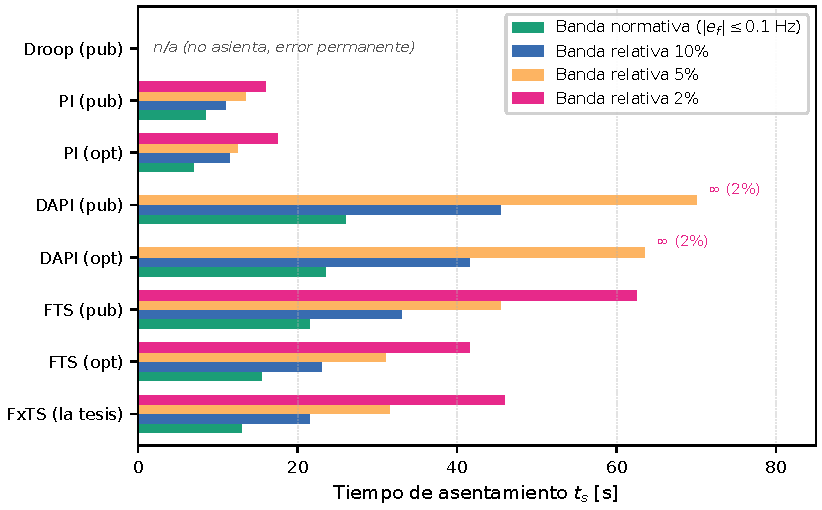
\includegraphics[width=0.95\textwidth]{Figuras/f5_1_tasas_asentamiento.pdf}
    \caption{Tiempos de asentamiento del nivel T1 por controlador y banda de evaluación: banda normativa de $0.100\text{ Hz}$ y bandas relativas de $10$, $5$ y $2$ por ciento. El estatismo puro no registra barra porque ninguna banda se cierra en la ventana de observación, y así se marca en el gráfico.}
    \label{fig:res_tasas_asentamiento}
\end{figure}

Tres lecturas se desprenden de la tabla. La primera es que el PI centralizado resultó el más rápido en la banda normativa, con $8.50\text{ s}$ en su variante publicada y $7.00\text{ s}$ en la optimizada, aunque su rapidez no viene acompañada de reparto de potencia, como se muestra en el apartado siguiente. La segunda es que el estatismo puro no asienta en ninguna de las cuatro bandas: sin lazo secundario, la desviación inducida por el estatismo es estacionaria por construcción y ninguna banda relativa llega a cerrarse dentro de la ventana. La tercera es la posición relativa del esquema propuesto: el FxTS asentó en $13.00\text{ s}$, esto es, $1.65$ veces más rápido que el FTS publicado ($21.50\text{ s}$) y $2$ veces más rápido que el DAPI publicado ($26.00\text{ s}$), sosteniendo además la banda del $2$ por ciento en $46.00\text{ s}$, donde el DAPI no la alcanza. La Figura~\ref{fig:res_tasas_asentamiento} ordena esas mismas mediciones por banda, de modo que se aprecia cuánto castiga cada exigencia adicional a cada controlador y en qué punto la comparación deja de ser posible porque ninguna banda llega a cerrarse.

Conviene subrayar el comportamiento del DAPI en la banda estrecha. Aunque aprueba el criterio normativo con $26.00\text{ s}$, su tiempo de asentamiento al $2$ por ciento es infinito en ambas variantes, lo que revela una cola de convergencia que la banda normativa no captura. El FTS y el FxTS, en cambio, cierran las cuatro bandas, y lo hacen en el orden esperado por la teoría: el esquema de tiempo fijo impone un plazo independiente del estado inicial, mientras que el de tiempo finito depende de la distancia inicial al equilibrio.

La comparación entre variantes publicada y optimizada aporta un dato adicional sobre la robustez de la sintonización. En el PI, la optimización mejoró la banda normativa de $8.50$ a $7.00\text{ s}$ pero degradó la banda del $2$ por ciento de $16.00$ a $17.50\text{ s}$, es decir, ganó velocidad inicial a costa de una cola más larga. En el DAPI y en el FTS el efecto fue uniforme, con mejoras en las cuatro bandas, mientras que el FxTS se reporta únicamente en su variante publicada porque el ajuste fino de sus exponentes no forma parte del alcance de esta validación. El estatismo, por su parte, no distingue entre variantes: ambas arrojan el mismo conjunto de valores, lo que confirma que su limitación no proviene de la sintonización sino de la ausencia de un lazo secundario.

\subsubsection{Calidad de reparto y estabilidad numérica}

La Tabla~\ref{tab:res_t1_calidad} reúne los seis indicadores restantes y el número de criterios aprobados por configuración. Las columnas $\Delta \eta_Q$ y $\Delta \eta_P$ cuantifican la dispersión del índice de utilización entre agentes; $e_V$ y $e_\omega$ son los errores residuales de tensión y frecuencia; CFL es el número espectral definido sobre \eqref{eq:cfl_condition}, y $\tau_{crit}$ el retardo crítico de \eqref{eq:tau_crit}. La abreviatura N/A señala que el indicador no es calculable por no existir capa de consenso distribuido o por no admitir el esquema un retardo finito de referencia.

\begin{table}[H]
    \centering
    \scriptsize
    \setlength{\tabcolsep}{3pt}
    \caption{Calidad de reparto, errores residuales, estabilidad numérica y criterios aprobados en el benchmark T1. CFL corresponde a la mitad del producto de \eqref{eq:cfl_condition}.}
    \label{tab:res_t1_calidad}
    \begin{tabularx}{\textwidth}{|>{\raggedright\arraybackslash}p{2.5cm}|>{\centering\arraybackslash}p{1.35cm}|>{\centering\arraybackslash}X|>{\centering\arraybackslash}X|>{\centering\arraybackslash}X|>{\centering\arraybackslash}X|>{\centering\arraybackslash}X|>{\centering\arraybackslash}X|>{\centering\arraybackslash}X|>{\centering\arraybackslash}p{1.55cm}|}
        \hline
        \textbf{Controlador} & \textbf{Modo} & \textbf{$\Delta f$ p-p (Hz)} & \textbf{$\Delta \eta_Q$} & \textbf{$\Delta \eta_P$} & \textbf{$e_V$ (p.u.)} & \textbf{$e_\omega$ (Hz)} & \textbf{CFL} & \textbf{$\tau_{crit}$ (ms)} & \textbf{Gates} \\
        \hline
        Droop puro & published & 0.0000 & 0.0800 & 0.1867 & 0.2000 & 0.4667 & 0.00 & N/A & 1 de 8 \\
        \hline
        Droop puro & optimized & 0.0000 & 0.0800 & 0.1867 & 0.2000 & 0.4667 & 0.00 & N/A & 1 de 8 \\
        \hline
        PI centralizado & published & 0.0000 & 0.0800 & 0.1867 & 0.0001 & 0.0000 & 0.25 & N/A & 5 de 8 (G8 no aplica) \\
        \hline
        PI centralizado & optimized & 0.0000 & 0.0800 & 0.1867 & 0.0000 & 0.0000 & 0.25 & N/A & 5 de 8 (G8 no aplica) \\
        \hline
        DAPI & published & 0.0120 & 0.0000 & 0.0000 & 0.0088 & 0.0236 & 0.16 & 2579.8 & 7 de 8 \\
        \hline
        DAPI & optimized & 0.0107 & 0.0000 & 0.0000 & 0.0067 & 0.0198 & 0.18 & 2299.8 & 7 de 8 \\
        \hline
        FTS & published & 0.0075 & 0.0000 & 0.0000 & 0.0000 & 0.0063 & 0.81 & 118.9 & 8 de 8 \\
        \hline
        FTS & optimized & 0.0017 & 0.0047 & 0.0047 & 0.0017 & 0.0009 & 1.60 & $-187.0$ & 6 de 8 \\
        \hline
        FxTS & published & 0.0029 & 0.0000 & 0.0000 & 0.0000 & 0.0018 & 0.84 & 96.3 & 8 de 8 \\
        \hline
    \end{tabularx}
\end{table}

\begin{figure}[H]
    \centering
    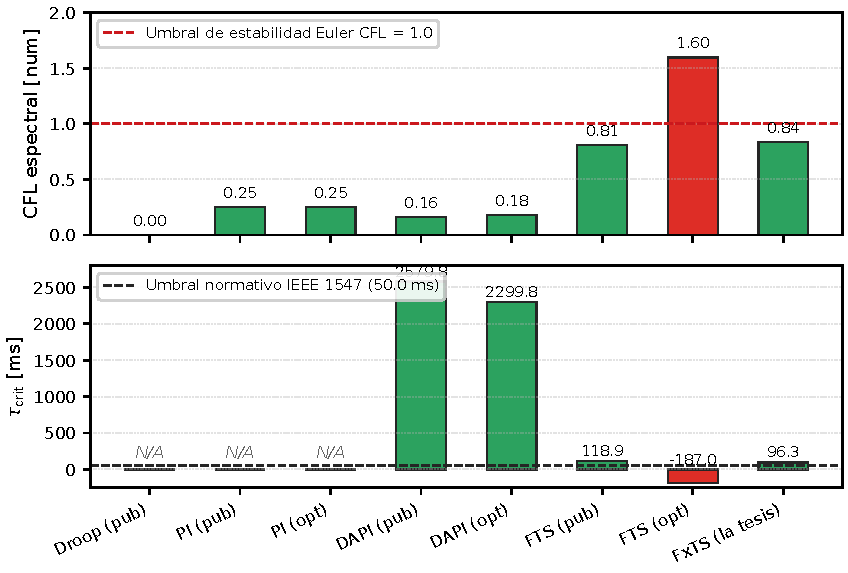
\includegraphics[width=0.95\textwidth]{Figuras/f5_6_estabilidad_numerica.pdf}
    \caption{Estabilidad numérica del benchmark T1. El panel superior compara el número CFL de cada configuración con el umbral unitario del criterio G7; el inferior, el retardo crítico con el umbral normativo de $50\text{ ms}$ del criterio G8. Las configuraciones sin capa de consenso distribuido no admiten retardo crítico y se marcan N/A, no cero.}
    \label{fig:res_estabilidad}
\end{figure}

El estatismo y el PI centralizado fallan G3 y G4 con idénticos valores de dispersión, $0.0800$ y $0.1867$ respectivamente. La causa no es un mal sintonizado sino estructural: ninguno de los dos esquemas incorpora acoplamiento entre vecinos, de modo que cada unidad se regula contra su propia referencia y la utilización relativa queda determinada por las impedancias y por los coeficientes de caída, no por un acuerdo explícito. El PI, en cambio, sí aprueba G1, G2, G5, G6 y G7, y su octavo criterio no aplica porque no existe capa de consenso distribuido sobre la cual definir un retardo crítico; de ahí el registro de $5$ de $8$ con la anotación correspondiente.

El DAPI invierte el patrón: reparte de forma ideal, con $\Delta \eta_Q$ y $\Delta \eta_P$ nulos en ambas variantes, y mantiene la desviación de frecuencia pico a pico en $0.0120\text{ Hz}$ y $0.0107\text{ Hz}$, valores reducidos frente al umbral de $0.200\text{ Hz}$. Sin embargo, falla G5 con $0.0088\text{ p.u.}$ en la variante publicada y $0.0067\text{ p.u.}$ en la optimizada, es decir, con un error de tensión entre una y dos veces el umbral de $0.005\text{ p.u.}$. El resultado es coherente con la naturaleza del lazo: la acción integral distribuida restituye la frecuencia y el reparto, pero no dispone de una señal de tensión con la misma autoridad, de manera que la regulación de magnitud queda rezagada.

El caso del FTS optimizado merece atención porque muestra que la optimización de ganancias puede comprar velocidad a costa de estabilidad numérica. Al elevar la ganancia, el esquema reduce el tiempo de asentamiento normativo de $21.50\text{ s}$ a $15.50\text{ s}$, pero viola G7 con un CFL de $1.60$ y G8 con un retardo crítico negativo de $-187.0\text{ ms}$. Un $\tau_{crit}$ negativo no significa que el lazo tolere retardos pequeños: significa que el esquema discreto ya es inestable en ausencia de retardo, y que ninguna reducción del mismo puede restituir la estabilidad. Sólo el FTS publicado y el FxTS publicado aprueban los ocho criterios, y lo hacen con márgenes distintos: el FxTS con CFL de $0.84$ y $\tau_{crit}$ de $96.3\text{ ms}$, el FTS con CFL de $0.81$ y $\tau_{crit}$ de $118.9\text{ ms}$. La Figura~\ref{fig:res_estabilidad} sitúa ambos indicadores frente a sus umbrales: en el panel superior el CFL de cada configuración contra la unidad, y en el inferior el retardo crítico frente a su umbral normativo, con las configuraciones que no admiten retardo marcadas como no aplicables en lugar de cero.

\subsubsection{Contraste con las cotas teóricas}

El primer contraste es el de la cota de Lyapunov. Para el grafo lineal de tres agentes, con conectividad algebraica $\lambda_2 = 1.0$, la cota de asentamiento derivada en el capítulo teórico es $T_f \le 52.54\text{ s}$, valor que coincide con el umbral del criterio G1. El FxTS asentó en $13.00\text{ s}$, esto es, un factor $4.04$ por debajo de la cota. La lectura correcta de ese factor no es que el algoritmo sea cuatro veces mejor de lo que promete, sino que la cota es un peor caso global construido para condiciones iniciales arbitrariamente alejadas del equilibrio, mientras que la operación de una microrred mantiene las desviaciones acotadas; la cota se cumple con holgura porque el régimen real es local.

El segundo contraste es el de la condición espectral. Con paso de discretización $\Delta t = 0.5\text{ s}$, autovalor máximo $\lambda_{\max}(\mathcal{H}) = 3.247$ y ganancia efectiva $g_{\text{ef}} = 1.033$ en el interior de la capa límite, el producto de \eqref{eq:cfl_condition} resulta $1.677$, inferior al límite de $2.0$ con un margen de $16.2$ por ciento, equivalente a un factor de $1.19$ entre el umbral y el valor efectivo. El CFL reportado en la Tabla~\ref{tab:res_t1_calidad} es precisamente ese producto dividido por dos, de donde resulta $0.84$; la normalización permite comparar el margen contra la unidad y explica por qué el umbral de G7 se fija allí y no en $2.0$.

El tercer contraste es el del retardo. La cota analítica de \eqref{eq:tau_crit} arroja $96.3\text{ ms}$ para la topología de validación, frente al umbral normativo de $50\text{ ms}$ adoptado en G8, lo que representa un factor de $1.93$ de holgura. El resultado es relevante porque el retardo crítico no se estimó por búsqueda empírica sino que se despejó de la misma condición de contracción que gobierna el CFL; ambos indicadores son, por tanto, dos vistas del mismo margen, y su consistencia mutua constituye una verificación cruzada del modelo de estabilidad.

\subsubsection{Validación del arnés mediante controles negativos}

Un benchmark que sólo reporta aprobados no demuestra que sepa reprobar. Por esa razón el arnés se sometió a cuatro controles negativos, cuyo propósito es verificar que el instrumento detecta las fallas que debe detectar y que el aprobado del esquema propuesto no es vacuo.

El control N1 anuló el consenso, dejando la ley de actualización sin término de vecinos. El resultado fue la ausencia de restitución: los errores residuales se mantuvieron en el valor inducido por el estatismo y ningún criterio de reparto se satisfizo. El control N2 sustituyó las ganancias por valores ajenos al diseño, $0.15$ y $0.85$, con los cuales el CFL igualó o superó la unidad y el esquema discreto perdió la contracción. El control N3 invirtió el signo del término restaurativo, lo que produjo divergencia y confirmó que la retroalimentación negativa es la que sostiene la convergencia. El control N4 empleó el DAPI como control positivo: al ser un esquema correctamente formulado, aprobó siete criterios y sólo quedó en reserva por G5, con un error de tensión de $0.0088\text{ p.u.}$.

El conjunto de los cuatro controles delimita el comportamiento del arnés: detecta la ausencia de acoplamiento, detecta el exceso de ganancia, detecta la inversión de signo y no penaliza indebidamente a un esquema ajeno bien formulado. El aprobado de ocho sobre ocho del FxTS se interpreta, por tanto, contra un instrumento que ya demostró saber fallar en las condiciones en que corresponde fallar.

\subsubsection{Experimento nodal de retenedores de frontera}

El benchmark no incorpora retenedores de frontera, pues opera con \texttt{boundary\_hold\_applied} en falso; el estudio de retenedores constituye, en consecuencia, un experimento nodal independiente y así se declara. El ensayo se ejecutó sobre el nodo solar de tipo Boost, con consigna de reactiva $Q_{\text{ref}} = 4000\text{ var}$, consigna activa $P_{\text{ref}} = 0\text{ W}$, irradiancia de $800\text{ W/m}^2$ y temperatura de $25$ grados. En $t = 40\text{ s}$ se impuso una caída de tensión a $0.8\text{ p.u.}$ con constante de $4.5\text{ s}$, y el registro se extendió durante $120\text{ s}$. Cada retenedor operó con paso de $0.5\text{ s}$ y se comparó contra una referencia calculada con paso de $0.05\text{ s}$, de manera que el error reportado mide el efecto de retener el estado de frontera durante un macro-paso completo.

\begin{table}[H]
    \centering
    \footnotesize
    \caption{Error de retención de la potencia del nodo solar Boost frente a la referencia de paso fino. El factor se calcula respecto del retenedor de orden cero.}
    \label{tab:res_retenedores}
    \begin{tabularx}{\textwidth}{|>{\raggedright\arraybackslash}p{3.6cm}|>{\centering\arraybackslash}X|>{\centering\arraybackslash}X|>{\centering\arraybackslash}X|}
        \hline
        \textbf{Retenedor} & \textbf{RMS (W)} & \textbf{Máximo (W)} & \textbf{Factor frente a ZOH} \\
        \hline
        ZOH & 3.85 & 26.65 & 1.00 \\
        \hline
        FROH $\lambda = 0.3$ & 7.45 & 110.31 & 1.93 \\
        \hline
        FROH $\lambda = 0.5$ & 10.80 & 166.09 & 2.80 \\
        \hline
        FROH $\lambda = 0.7$ & 14.33 & 221.87 & 3.72 \\
        \hline
        FROH $\lambda = 0.9$ & 17.93 & 277.65 & 4.65 \\
        \hline
        FOH ($\lambda = 1.0$) & 19.74 & 305.54 & 5.12 \\
        \hline
    \end{tabularx}
\end{table}

\begin{figure}[H]
    \centering
    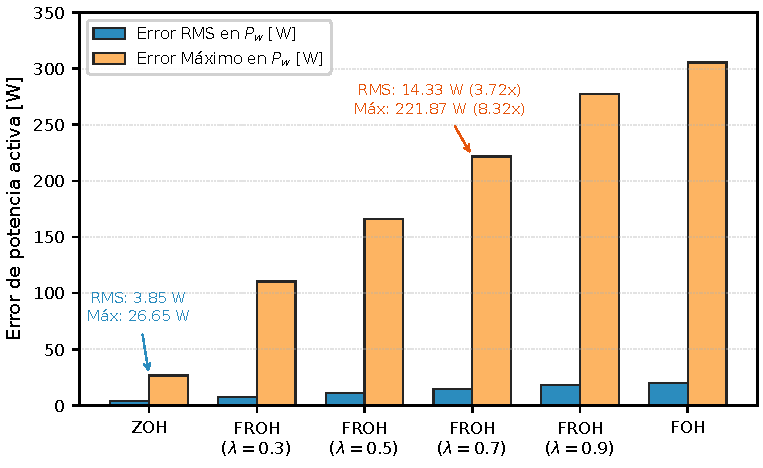
\includegraphics[width=0.95\textwidth]{Figuras/f5_7_retenedores.pdf}
    \caption{Error de retención de la potencia del nodo solar Boost para los seis esquemas evaluados, en RMS y en máximo frente a la referencia de paso fino. Las cifras anotadas coinciden con la Tabla~\ref{tab:res_retenedores}.}
    \label{fig:res_retenedores}
\end{figure}

El resultado contradice la expectativa habitual de que un retenedor de orden superior reduce el error de acoplamiento. El ZOH fue el más preciso de la serie, con un RMS de $3.85\text{ W}$ y un máximo de $26.65\text{ W}$, mientras que todas las variantes de extrapolación lo superaron, y el FOH elevó su error máximo a $305.54\text{ W}$ y su error RMS a $19.74\text{ W}$, esto es, un factor de $5.12$ sobre el RMS del ZOH. La explicación es mecánica: el retenedor implementado en el código extrapola con diferencia retrospectiva, es decir, opera como un predictor de primer orden construido sobre el último par de muestras. En una dinámica convexa como la caída de tensión con constante de $4.5\text{ s}$, la extrapolación lineal sobreestima sistemáticamente la señal, y el sesgo crece con el horizonte de predicción, que es precisamente lo que el parámetro $\lambda$ escala. La Figura~\ref{fig:res_retenedores} presenta la serie completa con el error RMS y el máximo en paralelo, de modo que se observa que el deterioro acompaña al parámetro de extrapolación y no se concentra en un caso aislado.

Debe precisarse que este retenedor no es el de Ishitobi, pese a la similitud de la nomenclatura. El esquema aquí evaluado no resuelve la condición de empalme de la trayectoria entre muestras, sino que prolonga la secante; su comportamiento es el de un predictor y no el de un reconstructor de orden fraccionario. El cociente máximo entre la señal retenida y la de referencia llegó a $8.33$ en el peor caso, lo que confirma que la extrapolación agresiva no es una mejora incremental sino una fuente de error dominante. La consecuencia práctica para la arquitectura de co-simulación es que el ZOH, pese a su simplicidad, constituye la opción conservadora y verificable, y que cualquier retenedor alternativo debería someterse a este mismo ensayo antes de adoptarse.

\subsection{Nivel T2: validación ciber-física en clúster HIL}

El nivel T2 traslada el esquema propuesto al hardware. El ensayo se ejecutó sobre el clúster de seis Raspberry Pi 5 y el PC Central, con la red de ocho barras, los recursos distribuidos en sus contenedores y la capa de comunicación ZeroMQ operando en modo lock-step. A diferencia del benchmark, aquí no hay variantes ni semillas: el ensayo de déficit es una sola ejecución de $300\text{ s}$ que se analiza por ventanas temporales, cada una asociada a un régimen operativo distinto. Ese ensayo cubre la primera de las tres familias del marco de evaluación, la de déficit de capacidad. La segunda, la de excedente de generación, cuenta con su escenario emitido e instalado pero no con corrida ejecutada, de modo que se declara con su criterio y sin cifras. La tercera, la de fallas de comunicación, se reporta con el ensayo de resiliencia que se describe en su apartado.

\subsubsection{Plataforma y contrato de muestreo}

El clúster se compone de seis Raspberry Pi 5 con direcciones \texttt{10.0.0.151} a \texttt{10.0.0.155} y \texttt{10.0.0.160}, coordinadas por el PC Central en \texttt{10.0.0.156} sobre una red Ethernet dedicada. La red eléctrica modelada es radial de baja tensión, con tensión nominal de $400\text{ V}$, ocho barras, siete ramas y potencia base de $10\text{ kVA}$. El contrato de muestreo establece $600$ pasos a $2\text{ Hz}$ con paso de $0.5\text{ s}$, lo que cubre $300\text{ s}$ de operación; la telemetría resultante consta de $600$ filas por $27$ columnas, con huella SHA-256 \texttt{bd71ba4a...}.

El paso correspondiente a $t = 0.0$ es un arranque plano previo al primer pulso del reloj ZeroMQ y, por esa razón, no se reporta: incluirlo introduciría en las estadísticas un estado que no pertenece a la operación del lazo cerrado. El ensayo se ejecutó sobre el escenario ESC-HIL-001\_rampa\_sombreado\_demanda, del que existe una versión consolidada —ESC-HIL-003\_consolidado\_rev5, la vigente en el banco— numéricamente equivalente: delta máximo nulo en las dieciocho series de entrada a lo largo de las $601$ muestras. Las series de irradiancia y de demanda que acompañan este capítulo provienen de los archivos consolidados de esa versión, de modo que las Figuras~\ref{fig:res_poa} y~\ref{fig:res_demanda} describen exactamente las entradas del ensayo. La ejecución se realizó con el lazo de potencia activa reconectado y con el anti-windup de $\pm 75\ \text{rad}$ de \eqref{eq:rest_local} en el integrador de frecuencia, de modo que la autoridad del agente quedó acotada durante los transitorios y no acumuló error mientras el actuador estaba saturado.

El contrato de muestreo merece una precisión adicional, porque de él depende la comparabilidad de las fases. Los $600$ pasos se ejecutaron en modo lock-step: el PC Central no avanzó al macro-paso siguiente hasta haber recibido las potencias de los seis nodos o hasta agotar el tiempo de espera configurado. Esa disciplina es la que permite afirmar que cada fila de la telemetría corresponde a un instante de simulación y no a un instante de llegada de mensajes, y es también la que sostiene la cadencia de $2\text{ Hz}$ como propiedad verificada y no como promedio. Las $27$ columnas registran, por nodo y por paso, las potencias activa y reactiva inyectadas, la magnitud y el ángulo de tensión de acoplamiento, la frecuencia local, los estados de consenso y los índices de utilización, de manera que cada afirmación de este apartado puede recalcularse a partir del archivo y no requiere del código que lo generó. Las Figuras~\ref{fig:res_poa} y~\ref{fig:res_demanda} recogen las series exógenas que gobiernan el ensayo, de modo que las respuestas de las fases siguientes puedan contrastarse contra la perturbación que las origina.

\begin{figure}[H]
    \centering
    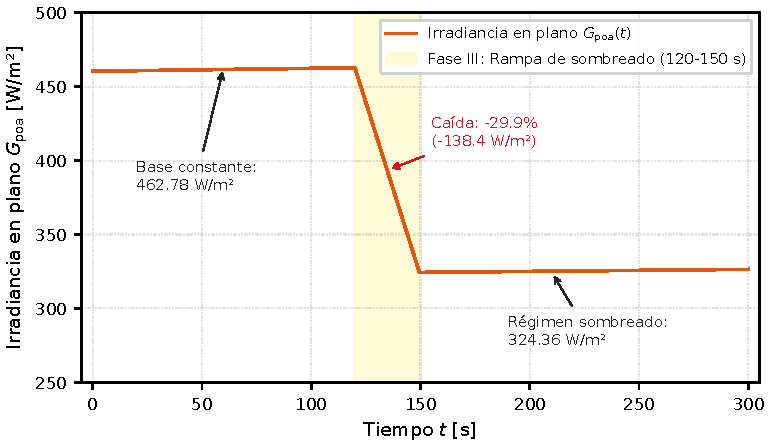
\includegraphics[width=0.95\textwidth]{Figuras/f5_8_poa.pdf}
    \caption{Irradiancia en el plano del arreglo durante los $300\text{ s}$ del ensayo, con la ventana de sombreado de la fase III delimitada. La serie se mantiene en $462.78\text{ W/m}^2$ hasta $t = 120\text{ s}$, desciende hasta $324.36\text{ W/m}^2$ en $t = 150\text{ s}$ y permanece constante el resto del ensayo; la caída es de $138.4\text{ W/m}^2$, el $29.9$ por ciento.}
    \label{fig:res_poa}
\end{figure}
\begin{figure}[H]
    \centering
    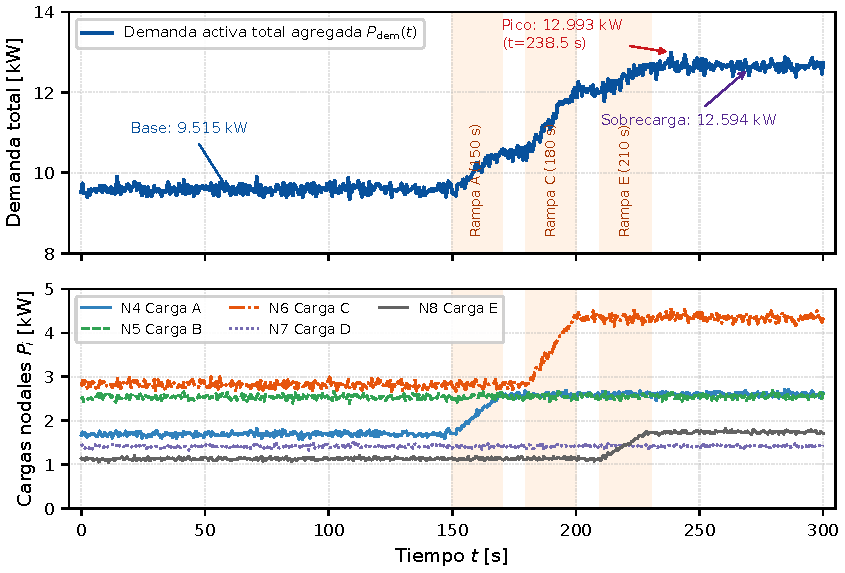
\includegraphics[width=0.95\textwidth]{Figuras/f5_9_demanda.pdf}
    \caption{Demanda del ensayo HIL. El panel superior muestra la demanda agregada, con la base de $9.515\text{ kW}$, el pico de $12.993\text{ kW}$ y el régimen de sobrecarga de $12.594\text{ kW}$, y señala el arranque de las tres rampas en $150$, $180$ y $210\text{ s}$; el panel inferior desglosa las cinco cargas nodales.}
    \label{fig:res_demanda}
\end{figure}

\subsubsection{Familia 1: déficit de capacidad}

La primera familia del marco reúne el ensayo en el que la demanda llega a exceder la capacidad firme del conjunto, de modo que la frecuencia no puede sostenerse sin la acción conjunta del estatismo primario y del lazo secundario. Su evidencia es una única ejecución sobre el clúster que se analiza en cinco ventanas temporales, cada una asociada a un régimen operativo distinto, y en un perfil de tensión nodal que se presenta al cierre de la familia.

\subsubsection{Fase I: acoplamiento y convergencia inicial}

La primera ventana abarca de $0.5$ a $25\text{ s}$ y corresponde al acoplamiento inicial entre el lazo físico y el lazo de consenso. La potencia neta intercambiada con la red osciló entre $-8.52$ y $+1.21\text{ kW}$, rango amplio que refleja la acomodación de los recursos desde el arranque plano hasta el punto de operación. La frecuencia registró su mínimo transitorio de $59.0556\text{ Hz}$ en $t = 9.0\text{ s}$.

El dato relevante de la fase es la convergencia del lazo reactivo. El consenso de reactiva convergió en el paso $21$, correspondiente a $t = 10.5\text{ s}$, con errores $e_{Q12}$ y $e_{Q23}$ iguales a $0.0000$. A partir de ese instante, el índice de utilización reactiva se mantuvo en $30.74$ por ciento en los tres inversores y así permaneció durante el resto del ensayo. La convergencia en $10.5\text{ s}$ debe contrastarse con la cota de $52.54\text{ s}$ del apartado anterior: el lazo físico converge dentro del plazo teórico y con un margen consistente con el factor observado en el benchmark. La Figura~\ref{fig:res_consenso_reactiva} registra ese cierre en sus dos paneles: la magnitud de los errores de consenso y los índices de utilización de los tres inversores, que dejan de separarse una vez alcanzada la convergencia.

El recorrido de la potencia neta en esta ventana, entre $-8.52$ y $+1.21\text{ kW}$, es propio del transitorio de acoplamiento y se atenúa una vez que el lazo secundario toma autoridad sobre las consignas. Su amplitud no indica una falla de reparto sino la acomodación de los convertidores desde el arranque plano, en el que ninguna unidad ha fijado aún su punto de operación. La excursión de $59.0556\text{ Hz}$ registrada en $t = 9.0\text{ s}$ es de amplitud comparable a la de la fase de sobrecarga y ocurre antes de que el consenso tome autoridad, lo que confirma que responde a la energización del conjunto y no a un déficit de capacidad. Las Figuras~\ref{fig:res_frecuencia_hil} y~\ref{fig:res_potencia_neta} amplían la mirada al registro completo: en la primera las cinco fases del banco quedan delimitadas, de modo que la excursión de esta ventana se compara con las posteriores; en la segunda las rampas de demanda se señalan sobre la traza de potencia neta.

\begin{figure}[H]
    \centering
    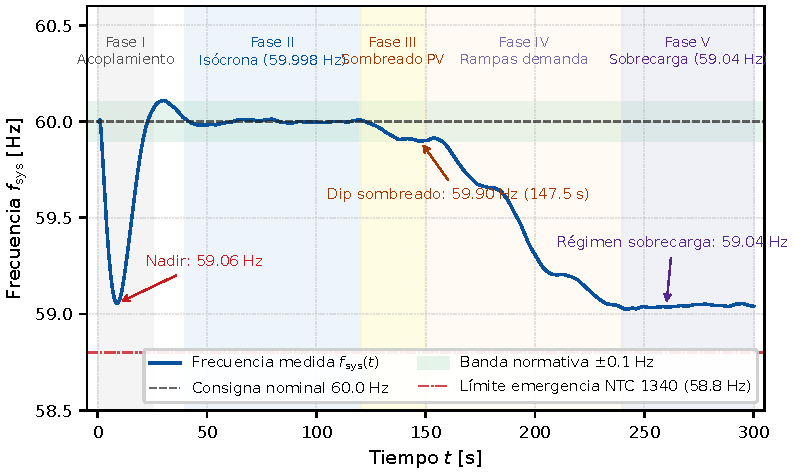
\includegraphics[width=0.95\textwidth]{Figuras/f5_2_frecuencia_hil.pdf}
    \caption{Frecuencia del sistema durante los $300\text{ s}$ del ensayo HIL, con las cinco fases del banco delimitadas por bandas sombreadas. Las guías horizontales señalan la ventana de la NTC 1340 y la banda fina de $0.1\text{ Hz}$; el eje vertical está restringido a la zona de interés y no cubre el rango completo de operación.}
    \label{fig:res_frecuencia_hil}
\end{figure}
\begin{figure}[H]
    \centering
    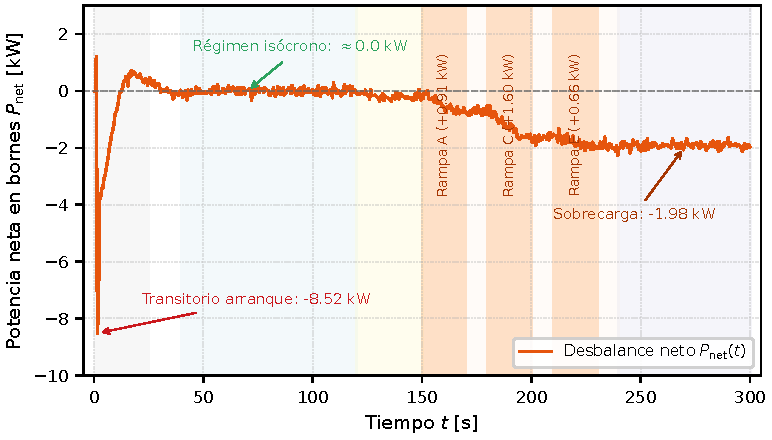
\includegraphics[width=0.95\textwidth]{Figuras/f5_3_potencia_neta.pdf}
    \caption{Potencia neta intercambiada con la red durante los $300\text{ s}$ del ensayo HIL. Las tres rampas de demanda se señalan sobre la traza y las anotaciones marcan el mínimo del transitorio de acoplamiento y el régimen de sobrecarga; el eje vertical es simétrico respecto de cero.}
    \label{fig:res_potencia_neta}
\end{figure}
\begin{figure}[H]
    \centering
    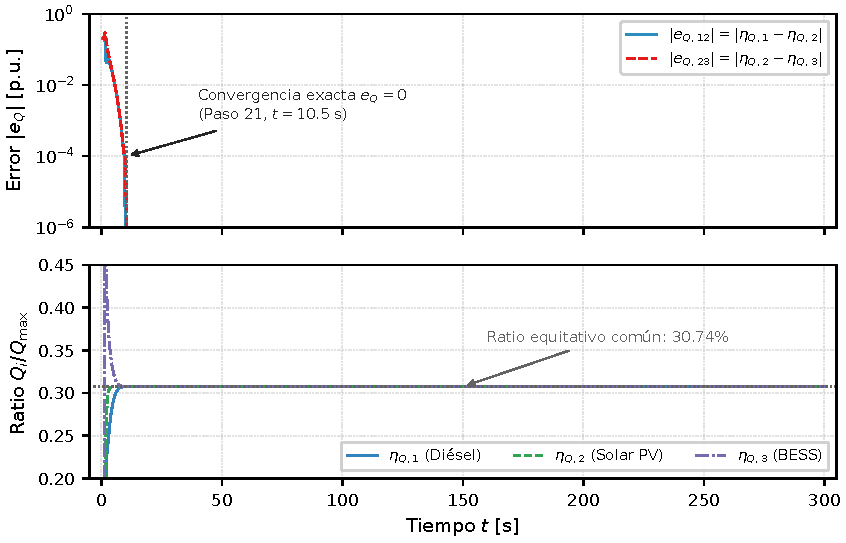
\includegraphics[width=0.95\textwidth]{Figuras/f5_5_consenso_reactiva.pdf}
    \caption{Consenso de potencia reactiva en el ensayo HIL, durante los $300\text{ s}$ del registro. El panel superior muestra la magnitud de los errores de consenso en escala logarítmica; el inferior, los índices de utilización reactiva de los tres inversores. La convergencia exacta de ambos errores se alcanza en el paso 21.}
    \label{fig:res_consenso_reactiva}
\end{figure}

\subsubsection{Fase II: régimen isócrono}

Entre $40$ y $120\text{ s}$ el sistema operó en régimen isócrono. La frecuencia se mantuvo en $59.9983 \pm 0.0082\text{ Hz}$, con un mínimo de $59.9815\text{ Hz}$ y un máximo de $60.0139\text{ Hz}$; la desviación media respecto de $60.0\text{ Hz}$ fue de $0.0017\text{ Hz}$. La potencia neta promedió $-0.0027\text{ kW}$, con un rango de $-0.32$ a $+0.29\text{ kW}$, y la demanda agregada promedió $9.5983\text{ kW}$, con valores entre $9.3417$ y $9.8969\text{ kW}$. La interpretación de esta ventana es directa: el lazo integral del generador diésel sostiene el punto isócrono, de modo que la frecuencia permanece próxima a la nominal sin que el consenso deba intervenir con autoridad adicional. La dispersión observada corresponde al ruido de cuantización del reloj y no a una oscilación de lazo, y la irradiancia se mantiene constante a lo largo de todo el intervalo, de modo que ninguna perturbación de recurso actúa todavía sobre el sistema.

\subsubsection{Fase III: sombreado fotovoltaico}

Entre $120$ y $150\text{ s}$ el escenario aplica la rampa de sombreado fotovoltaico definida en ESC-HIL-001, que no constituye una contingencia no modelada sino una perturbación declarada del guion de ensayo. Hasta $t = 120\text{ s}$ la irradiancia se mantiene en $462.78\text{ W/m}^2$; a partir de ese instante desciende de forma continua hasta $324.36\text{ W/m}^2$ en $t = 150\text{ s}$, esto es, una reducción de $138.42\text{ W/m}^2$ equivalente al $29.91$ por ciento en treinta segundos, y desde ahí permanece constante. La Figura~\ref{fig:res_poa} presenta esa rampa sobre el registro completo del ensayo. La demanda agregada no cambia en esta ventana: promedia $9.5875\text{ kW}$ y oscila entre $9.3935$ y $9.7886\text{ kW}$. La perturbación es, por tanto, de recurso y no de carga, condición que permite atribuirle el desplazamiento de frecuencia que se observa a continuación.

La consecuencia medida es un descenso de la frecuencia a $59.9394 \pm 0.0373\text{ Hz}$, con mínimo de $59.8979\text{ Hz}$ en $t = 147.5\text{ s}$, equivalente a una desviación de $0.1021\text{ Hz}$ respecto de la nominal. La potencia neta promedia $-0.1769\text{ kW}$ y alcanza su mínimo de $-0.37\text{ kW}$ en $t = 130.5\text{ s}$. La frecuencia cruza la banda de $0.100\text{ Hz}$ en $t = 146.5\text{ s}$, sin que se registre desconexión de carga ni actuación de protecciones. La correlación entre irradiancia y frecuencia en esta ventana es de $+0.954$, frente a $+0.313$ en la ventana isócrona, donde la irradiancia es constante; ese contraste sostiene la atribución causal.

La interpretación física concuerda con la magnitud del fenómeno. La caída de generación fotovoltaica es del orden de $0.23\text{ kW}$ y la absorbe el respaldo proporcional del diésel, cuyo aporte es $\kappa_{p,\omega} e_\omega \approx 95\text{ W}$ para la desviación media y $\approx 160\text{ W}$ en el mínimo, del mismo orden que el desbalance medido. El lazo integral no alcanza a cerrar el error antes de que comiencen las rampas de demanda de la fase siguiente, de manera que el sistema llega a esa fase con un desplazamiento cercano a $0.10\text{ Hz}$ que no le corresponde.

\subsubsection{Fase IV: perturbaciones de demanda}

Entre $150$ y $238.5\text{ s}$ se inyectaron tres rampas de demanda de $20\text{ s}$ de duración cada una: en el nodo N4 un incremento de $0.906\text{ kW}$ entre $150$ y $170\text{ s}$; en el nodo N6 un incremento de $1.596\text{ kW}$ entre $180$ y $200\text{ s}$; y en el nodo N8 un incremento de $0.657\text{ kW}$ entre $210$ y $230\text{ s}$. La Figura~\ref{fig:res_demanda} sitúa las tres rampas sobre la demanda agregada y desglosa las cinco cargas nodales. Aquí comienza la componente de demanda de la perturbación, sobre un sistema que ya venía desplazado en cerca de $0.10\text{ Hz}$ por el sombreado de la fase anterior. Las tres rampas se suceden sin solaparse entre sí, lo que permitió observar la respuesta del lazo integral a medida que la carga crecía de forma escalonada.

La demanda agregada pasó de $9.515\text{ kW}$ a $12.594\text{ kW}$ en $t = 240\text{ s}$, con un pico de $12.993\text{ kW}$ en $t = 238.5\text{ s}$ asociado al último escalón de la rampa. El incremento total, del orden de $3.5\text{ kW}$ sobre una base de $9.515\text{ kW}$, sometió a los recursos a una exigencia superior a su capacidad firme, situación que se resolvió en la fase siguiente y que constituye el fenómeno central de la validación en hardware.

La respuesta durante las rampas conservó la forma prevista: la frecuencia descendió de manera gradual mientras la demanda crecía, el reparto activo se mantuvo equitativo entre los agentes y la tensión nodal no se separó de la referencia. La suavidad de la excursión se explica por la duración de cada rampa, de $20\text{ s}$, muy superior a la constante de tiempo del lazo secundario, de modo que el consenso dispuso de tiempo para redistribuir la carga sin que el sistema operara fuera de su punto de equilibrio cuasiestático. Al finalizar la tercera rampa, sin embargo, la demanda superó el techo de capacidad y el régimen cambió de naturaleza.

\subsubsection{Fase V: sobrecarga y transición al estatismo primario}

Entre $240$ y $300\text{ s}$ el sistema operó en sobrecarga. La frecuencia se estabilizó en $59.0414 \pm 0.0076\text{ Hz}$, con un mínimo de $59.0247\text{ Hz}$ en $t = 242.0\text{ s}$, correspondiente al paso $484$. La potencia neta fue de $-1.980\text{ kW}$ en $t = 240\text{ s}$ y de $-1.970\text{ kW}$ en $t = 300\text{ s}$, es decir, prácticamente constante a lo largo de la ventana.

La deducción de esta condición operativa se desarrolla a continuación. La potencia generada real resultó de descontar a la demanda el intercambio neto con la red:

\begin{equation}
P_{\text{gen}} = P_{\text{dem}} - P_{\text{net}} = 12.594 - 1.980 = 10.614\ \text{kW}
\end{equation}

Esa potencia se repartió entre los tres recursos del banco. El nodo solar aportó $0.535\text{ kW}$ con una irradiancia cercana a $325.6\text{ W/m}^2$, el BESS entregó $1.500\text{ kW}$, valor que corresponde a su límite continuo, y el diésel asumió el resto con $8.579\text{ kW}$ eléctricos:

\begin{equation}
P_{\text{eje}} = \frac{8.579}{0.95} = 9.03\ \text{kW}
\end{equation}

donde $0.95$ es el rendimiento adoptado para el conjunto generador. La capacidad firme a $60.0\text{ Hz}$ se obtiene sumando la capacidad del diésel, la del BESS y el aporte solar disponible:

\begin{equation}
P_{\text{firme}} = 9.500 + 1.500 + 0.535 = 11.535\ \text{kW}
\end{equation}

de modo que el déficit de capacidad frente a la demanda de la fase resulta:

\begin{equation}
\Delta P = P_{\text{dem}} - P_{\text{firme}} = 12.594 - 11.535 = -1.059\ \text{kW}
\end{equation}

El déficit explica la caída de frecuencia sin necesidad de invocar una falla del algoritmo. Para verificarlo, se contrastó el valor medido con la predicción de la ecuación de oscilación \eqref{eq:swing}, evaluada con potencia base de $10\text{ kVA}$ y coeficiente de amortiguamiento de $12$:

\begin{equation}\label{eq:res_swing_pred}
f_{\text{pred}} = 60.0 + \frac{1}{12}\cdot\frac{-1.980}{10}\cdot 60.0 = 59.010\ \text{Hz}
\end{equation}

La predicción de $59.010\text{ Hz}$ corresponde al valor de régimen permanente del modelo rígido. La frecuencia medida, $59.0414\text{ Hz}$, se ubica por encima de esa predicción porque la señal atraviesa el filtro pasa-bajos de constante $2.0\text{ s}$ antes de ser registrada, lo que suaviza el escalón y reduce la excursión. La convergencia entre ambos valores, del orden de tres centésimas de hercio, confirma que la ecuación de oscilación describe adecuadamente el fenómeno y que la diferencia es atribuible al filtrado de medición y no a una dinámica no modelada.

El respaldo proporcional del diésel se verificó sobre el estatismo de \eqref{eq:droop_w}. Con una desviación de frecuencia de $6.023\text{ rad/s}$ respecto de la referencia y la ganancia $\kappa_{p,\omega} = 250.0\ \text{W/(rad/s)}$ declarada en \eqref{eq:rest_local}, la potencia adicional entregada por el gobernador resulta:

\begin{equation}
P_{\text{res}} = 250.0 \times 6.023 = 1505.7\ \text{W}
\end{equation}

Este respaldo, sumado al punto de operación previo del generador, es el que sostiene la frecuencia en $59.04\text{ Hz}$ en lugar de permitir una caída mayor. La transición hacia el estatismo primario fue monótona: no se observaron ciclos límite, ni oscilaciones sostenidas, ni actuación del relé de subfrecuencia.

\subsubsection{Perfil de tensión nodal}

La tensión en las ocho barras se mantuvo entre $0.99965$ y $1.00462\text{ p.u.}$, es decir, entre $399.86$ y $401.85\text{ V}$ sobre la base de $400\text{ V}$. El rango completo de variación nodal fue, por tanto, inferior a medio punto porcentual, muy por debajo de la tolerancia de $\pm 5$ por ciento que admiten IEEE 1547 y la norma NTC 1340. El resultado es consistente con la operación del lazo de restitución de tensión: el error $e_V$ reportado en el benchmark fue nulo, y en el banco la tensión no llegó a separarse de la referencia en ninguna barra ni durante las rampas de demanda. La Figura~\ref{fig:res_tensiones} recoge la envolvente de las ocho barras a lo largo del ensayo con el eje vertical ampliado a la zona de interés, de modo que se aprecia la forma de la variación aunque el margen frente a la tolerancia regulatoria no resulte visible a esa escala.

\begin{figure}[H]
    \centering
    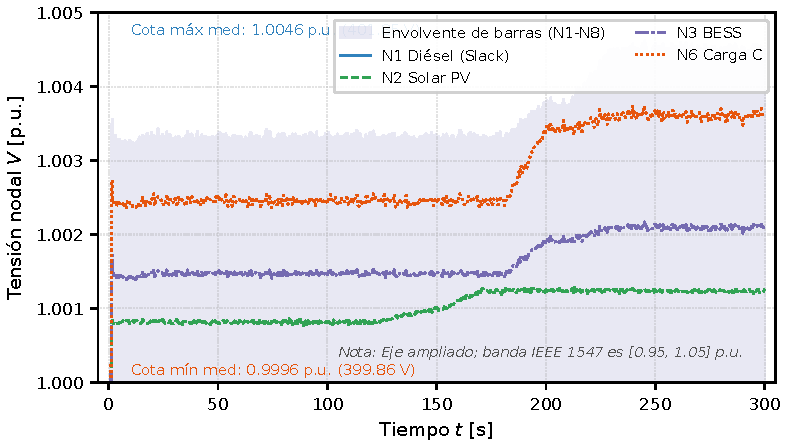
\includegraphics[width=0.95\textwidth]{Figuras/f5_4_tensiones_nodales.pdf}
    \caption{Envolvente de tensión de las ocho barras durante el ensayo HIL. El eje vertical está ampliado a la zona de interés, de $1.000$ a $1.005\text{ p.u.}$, y por tanto no representa la tolerancia completa de $\pm 5$ por ciento de IEEE 1547 y NTC 1340.}
    \label{fig:res_tensiones}
\end{figure}

\subsubsection{Familia 2: excedente de generación}

La segunda familia del marco de evaluación invierte el signo del balance. En ella la demanda nunca supera la generación disponible, de modo que la frecuencia no está en riesgo por insuficiencia, pero la generación sí puede superar la demanda y el excedente debe absorberse o recortarse. El escenario correspondiente está emitido e instalado, pendiente de ensayo, y exige una ventana declarada con irradiancia elevada y demanda plana o descendente: la perturbación inversa a la del ensayo anterior, donde el sombreado redujo la generación manteniendo la carga constante.

Lo que se medirá en esa ventana es, primero, la frecuencia sostenida dentro de $\pm 0.05\ \text{Hz}$ de la nominal; segundo, el reparto equitativo del exceso entre la carga de la batería y el recorte de la fuente fotovoltaica, con un índice de utilización propio y un error de consenso de la misma cota que el de la reactiva; y tercero, la ausencia de saturación de la absorción salvo en el límite declarado del BESS. Ambas capacidades están implementadas en la plataforma: el BESS admite consigna de absorción acotada por su estado de carga —nula en $0.20$, escalada linealmente hasta $0.90$ en descarga y decreciente entre $0.85$ y $0.95$ en carga—, y el nodo fotovoltaico admite un techo de inyección expresado como fracción del punto de máxima potencia. El exceso entra al mismo mecanismo de reparto que la reactiva, con un índice de utilización propio. Lo que falta es la corrida: el escenario con ventana excedentaria está emitido e instalado y su ensayo sigue pendiente, de modo que la familia se declara con su escenario y su criterio y sin resultados, y no se reporta cifra alguna hasta que el ensayo se publique.

\subsubsection{Familia 3: fallas de comunicación}

La tercera familia somete el lazo de consenso a la degradación de la red de comunicación, que es la contingencia que el cuarto objetivo específico compromete. El ensayo se ejecutó sobre el ejecutor de la plataforma con inyección programada de fallas, conforme al contrato de contingencias, con $601$ muestras a $2\ \text{Hz}$ durante $300\ \text{s}$ y semilla base $42$. Se compone de cuatro tramos: referencia sin falla en $[0, 100)\ \text{s}$; rampa de latencia estocástica de $50$ a $500\ \text{ms}$ en $[100, 200)\ \text{s}$; pérdida de paquetes del $20$ por ciento en ambos sentidos del enlace entre los nodos 2 y 3; y desconexión total del enlace entre los nodos 1 y 2 durante $30\ \text{s}$, entre $200$ y $300\ \text{s}$.

Los resultados separan con claridad los dos efectos. El error de consenso de reactiva se mantuvo en cero en los tres tramos: su máximo fue de $0.0009$ en el tramo nominal y de $0.0000$ en los dos tramos con falla inyectada. La frecuencia mínima del registro fue de $59.9894\ \text{Hz}$ en $t = 58\ \text{s}$, es decir, dentro del tramo sin falla; en los tramos degradados no descendió de $59.9935\ \text{Hz}$, de modo que la ventana de la NTC 1340 se respetó con holgura durante todo el ensayo. De los $3606$ paquetes intentados se entregaron $3412$ y se descartaron $194$, un $5.38$ por ciento concentrado en las ventanas de falla.

Los cuatro criterios de la familia se cumplen en este ensayo: el error de consenso retorna a cero después de cada tramo dentro del horizonte del lazo secundario; la frecuencia no abandona la ventana normativa; la reconvergencia se completa sin intervención externa; y, tras la desconexión, el lazo vuelve a operar con el enlace restablecido. La razón es estructural y no accidental: durante los $30\ \text{s}$ de corte el búfer retuvo el último estado recibido de cada vecino, y como el consenso se evalúa una vez por macro-paso mientras los mensajes se entregan de forma asíncrona, un paquete perdido no se propaga como error de estado. El ensayo se ejecutó sobre el ejecutor de la plataforma; su réplica sobre el clúster físico de seis nodos y la campaña de semillas múltiples quedan fuera de este capítulo.

\subsection{Discusión integrada}

\subsubsection{Qué demuestra cada nivel y qué no}

El nivel T1 demuestra que el esquema propuesto se compara favorablemente contra cinco arquitecturas de control secundario bajo criterios idénticos, reproducibles y verificables. Lo hace sobre una planta algebraico-cinemática, con semilla fija y con ocho criterios definidos antes de la ejecución; en consecuencia, demuestra superioridad algorítmica en el sentido acotado de la palabra: mejor desempeño bajo ese modelo, esos criterios y esa perturbación. No demuestra comportamiento electromagnético, ni tolerancia a retardos reales, ni capacidad de operar en tiempo real.

El nivel T2 demuestra lo complementario: que el esquema sostiene una cadencia determinista de $2\text{ Hz}$ durante $300\text{ s}$, que el consenso converge sobre una red física con flujo de potencia resuelto, y que el sistema responde a perturbaciones de demanda reales sin perder el reparto ni la estabilidad. No demuestra superioridad algorítmica, porque en el banco sólo se ejecutó el esquema propuesto, con una sola planta y un solo escenario.

La combinación es lo que sostiene la tesis. T1 sin T2 sería una comparación de algoritmos en un mundo sin física; T2 sin T1 sería una demostración de viabilidad sin término de comparación. Juntos permiten afirmar que el esquema es simultáneamente mejor que sus alternativas bajo criterios homogéneos y capaz de operar sobre hardware real en condiciones de red.

\subsubsection{La caída a 59.04 Hz como límite de capacidad y no del algoritmo}

El resultado más susceptible de mala interpretación es la frecuencia de $59.04\text{ Hz}$ en la fase de sobrecarga. Una lectura apresurada la atribuiría a una insuficiencia del lazo de consenso; la evidencia disponible indica lo contrario. El consenso de reactiva había convergido a error nulo desde $t = 10.5\text{ s}$ y el reparto se mantuvo durante toda la sobrecarga, de modo que el lazo distribuido hizo exactamente lo que le correspondía: igualar la utilización relativa de los recursos. La frecuencia cayó porque la demanda excedió la capacidad firme en $1.059\text{ kW}$, y ninguna ley de reparto puede suministrar potencia que los recursos no tienen.

La distinción importa porque separa dos dominios de validez. El reparto es un problema de coordinación y se resuelve con información; la suficiencia es un problema de capacidad y se resuelve con inversión o con despacho. El ensayo demuestra que el primero funciona incluso cuando el segundo falla, que es precisamente la condición deseable en una microrred: el control no enmascara el límite físico ni lo agrava con un reparto inequitativo.

El valor de $59.04\text{ Hz}$ cumple además con la norma NTC 1340, cuya ventana de cumplimiento es de $\pm 2$ por ciento sobre $60.0\text{ Hz}$, es decir, $[58.8, 61.2]\text{ Hz}$. La transición hacia ese punto fue monótona, sin ciclos límite ni desconexión de cargas, y el relé de subfrecuencia, ajustado en $[57.0, 63.0]\text{ Hz}$, no llegó a actuar. La caída es, por tanto, un límite de capacidad declarado y no una falla del algoritmo.

Conviene explicitar el contrafactual, porque precisa el alcance de la conclusión. Si la capacidad firme hubiera sido superior en $1.059\text{ kW}$, el mismo lazo habría sostenido la frecuencia en torno a la nominal sin cambio alguno de sintonización, pues el reparto ya estaba resuelto y el error de frecuencia del consenso era nulo. La variable que explica el resultado es, entonces, la suficiencia del parque y no la ley de control. Esa separación es la que permite recomendar el esquema para microrredes con margen de capacidad y, al mismo tiempo, identificar el dimensionamiento como la acción correctiva cuando el margen no existe.

\subsubsection{Validez, límites y amenazas a la validez}

La validez interna del nivel T1 descansa en la identidad de planta, semilla y secuencia de eventos entre configuraciones, y en la existencia de cuatro controles negativos que verifican la sensibilidad del arnés. Su límite principal es que se apoya en una sola semilla: las cifras aquí presentadas describen una realización determinista y no una distribución. Lo que este capítulo valida es la convergencia de los cuatro estados de consenso en el nivel T1 —tensión y frecuencia dentro de la banda normativa— y, en el banco físico, la convergencia del consenso de reactiva junto con la regulación de frecuencia por el lazo integral del diésel. Las familias 2 y 3 del marco de evaluación se tratan por separado y con estatuto distinto. La de excedente cuenta con la capacidad implementada —absorción en el BESS y recorte de la fuente fotovoltaica— y con dos escenarios emitidos, el perfil con ventana declarada y su referencia sin excedente, pero su corrida no se ha ejecutado, de modo que no se publica cifra alguna. La de fallas de comunicación se reporta en su apartado con un ensayo de $300\ \text{s}$; su réplica sobre el clúster físico y la campaña de semillas múltiples quedan fuera de este capítulo y se declaran como trabajo pendiente.

La validez del nivel T2 descansa en la trazabilidad criptográfica de la telemetría y en la operación real del reloj y de la red. Su límite es el escenario único: ESC-HIL-001 no agota el espacio de contingencias, y un banco de mayor tamaño —el de $21$ nodos— se declara explícitamente como trabajo futuro. Tampoco debe extrapolarse el resultado a topologías malladas, pues la red ensayada es radial por diseño.

Una tercera amenaza a la validez afecta la interpretación conjunta de los dos niveles. El retenedor de frontera no se ejecuta en el benchmark, porque \texttt{boundary\_hold\_applied} es falso; en consecuencia, la comparación de retenedores de la Tabla~\ref{tab:res_retenedores} no forma parte del benchmark sino que constituye un experimento nodal independiente, y así se declara para evitar que se le atribuya un alcance que no tiene. Del mismo modo, la planta del nivel T1 es algebraico-cinemática según la decisión D-13, de manera que sus cifras de estabilidad numérica describen el esquema de integración y no la dinámica de los convertidores.

\subsection{Síntesis de resultados}

La Tabla~\ref{tab:res_sintesis} cruza las seis dimensiones evaluadas con la evidencia disponible en cada nivel. La columna final indica la fuente de la cifra, con el objeto de que el lector pueda verificar qué afirmaciones se sostienen en el benchmark, cuáles en la telemetría del banco y cuáles en ambos.

\begin{table}[H]
    \centering
    \footnotesize
    \caption{Síntesis de resultados por dimensión y nivel de validación, con indicación de la fuente de evidencia.}
    \label{tab:res_sintesis}
    \begin{tabularx}{\textwidth}{|>{\raggedright\arraybackslash}p{2.4cm}|>{\raggedright\arraybackslash}X|>{\raggedright\arraybackslash}X|>{\raggedright\arraybackslash}p{2.8cm}|}
        \hline
        \textbf{Dimensión} & \textbf{Nivel T1} & \textbf{Nivel T2} & \textbf{Evidencia} \\
        \hline
        Rapidez & $13.00\text{ s}$ del FxTS, factor $4.04$ bajo la cota & Convergencia de reactiva en $10.5\text{ s}$ & metrics.json y telemetría \\
        \hline
        Reparto & $\Delta \eta = 0.0000$ & Error $e_Q = 0.0000$ con ratio de $30.74$ por ciento & Ambas fuentes \\
        \hline
        Estabilidad numérica & CFL de $0.84$ con margen de $16.2$ por ciento & Cero saturación y sin ciclos límite & Ambas fuentes \\
        \hline
        Robustez a retardo & $\tau_{crit}$ de $96.3\text{ ms}$, mayor o igual a $50\text{ ms}$ & Cadencia de $2\text{ Hz}$ sostenida $300\text{ s}$ & Ambas fuentes \\
        \hline
        Tensión & $e_V = 0.0000$ & Tensión entre $0.99965$ y $1.00462$ p.u. & Ambas fuentes \\
        \hline
        Límite físico & No aplica & Capacidad firme de $11.535\text{ kW}$ con desbalance de $-1.980\text{ kW}$ & Telemetría \\
        \hline
        Excedente de generación & No evaluado & Absorción y recorte implementados; ensayo pendiente & Pendiente \\
        \hline
        Fallas de comunicación & No evaluado & Validado: $e_Q$ máximo $0.0000$ con $5.38$ por ciento de paquetes perdidos & Campaña de resiliencia \\
        \hline
    \end{tabularx}
\end{table}


Los hallazgos que se desprenden del cruce son los siguientes:

\begin{itemize}
    \item El esquema de consenso en tiempo fijo aprobó los ocho criterios del benchmark con CFL de $0.84$ y $\tau_{crit}$ de $96.3\text{ ms}$, y fue el único, junto con el FTS publicado, en hacerlo sin ceder reparto ni margen numérico.
    \item El FxTS asentó en $13.00\text{ s}$, un factor de $4.04$ por debajo de la cota de Lyapunov de $52.54\text{ s}$ y $1.65$ veces más rápido que el FTS publicado, lo que confirma que la cota es un peor caso global y no una predicción de operación.
    \item El reparto proporcional se sostuvo en ambos niveles: dispersión nula de los índices en T1 y ratio de $30.74$ por ciento idéntico en los tres inversores del banco, desde $t = 10.5\text{ s}$ hasta el final del ensayo.
    \item La caída a $59.0414\text{ Hz}$ en la fase de sobrecarga se explica por un déficit de capacidad de $1.059\text{ kW}$ y no por una falla del lazo, y la predicción de la ecuación de oscilación \eqref{eq:res_swing_pred}, $59.010\text{ Hz}$, reprodujo el fenómeno dentro del error atribuible al filtrado de medición.
    \item La tensión nodal permaneció entre $0.99965$ y $1.00462\text{ p.u.}$ en las ocho barras, dentro de las tolerancias de IEEE 1547 y NTC 1340, sin que la sobrecarga activa comprometiera el perfil de magnitud.
    \item El retenedor de frontera no mejora el acoplamiento en este banco: el ZOH resultó el más preciso y el FOH multiplicó por $5.12$ su error RMS, de modo que la extrapolación se descarta como opción por defecto en la arquitectura de co-simulación.
\end{itemize}

\subsection{Cierre del capítulo y trabajo pendiente}

Este capítulo no se cierra con conclusiones, y la razón es verificable en el marco de evaluación: dos de las tres familias de prueba siguen sin ensayo ejecutado. La familia de excedente de generación cuenta con la capacidad implementada y con dos escenarios emitidos e instalados —el perfil con ventana declarada y su referencia sin excedente—, pero ninguno se ha corrido, de modo que la absorción en la batería y el recorte de la fuente fotovoltaica no tienen todavía evidencia empírica. La familia de fallas de comunicación sí tiene el ensayo que se reporta en este capítulo, ejecutado sobre el ejecutor de la plataforma con inyección programada de fallas, pero su réplica sobre el clúster físico de seis nodos y la campaña de semillas múltiples permanecen pendientes.

Consolidar conclusiones antes de esas dos corridas afirmaría más de lo que la evidencia sostiene. Lo que este capítulo establece es el desempeño del esquema propuesto en el benchmark numérico, en el banco de hardware en el lazo bajo la familia de déficit y en la campaña de resiliencia sobre el ejecutor; lo que falta es la ejecución que permita cerrar el balance de las tres familias y, con él, las conclusiones y el trabajo futuro del documento.


\renewcommand{\refname}{REFERENCIAS}
\addcontentsline{toc}{section}{REFERENCIAS}

\bibliographystyle{apalike} 
\bibliography{TuArchivo}

\end{document}